% !Mode:: "TeX:UTF-8"

% 定义编译方式 dvipdfmx 或者 pdflatex,默认为 dvipdfmx
% 方式编译,如果需要修改,只需改变花括号中的内容即可。
%\def\usewhat{pdflatex}

% book作为文档类
% 插入空白页可以设置openright
%\documentclass[12pt,openany,oneside]{book}
\documentclass[UTF8,12pt,openany,oneside]{book}

% 定义本文所使用宏包
% !Mode:: "TeX:UTF-8"

% 原作者信息Original Authors:
% 张井   Jing Zhang: prayever@gmail.com     天津大学2010级管理与经济学部信息管理与信息系统专业硕士生
% 余蓝涛 Lantao Yu: lantaoyu1991@gmail.com  天津大学2008级精密仪器与光电子工程学院测控技术与仪器专业本科生

% Thanks 中大移植版by林海涛&徐浩晖&

%%%%%%%%%% Package %%%%%%%%%%%%

% 支持插图处理
\usepackage{graphicx}
% 控制文档布局
%\usepackage[a4paper,text={146.4 true mm,239.2 true mm},top= 26.2 true mm,left=31.8 true mm,head=6 true mm,headsep=6.5 true mm,foot=16.5 true mm]{geometry}
\usepackage[a4paper,text={146.4 true mm,239.2 true mm},top= 26.2 true mm,left=31.8 true mm,head=6 true mm,headsep=6.5 true mm,foot=16.5 true mm,footnotesep=-8 true mm]{geometry}

% 支持版面尺寸设置
% 支持国际标准单位
\usepackage[squaren]{SIunits}               

\usepackage{titletoc}                       % 控制目录的宏包
\usepackage[raggedleft]{titlesec}               % 控制标题的宏包

\usepackage{fancyhdr}                       % fancyhdr宏包 支持页眉和页脚的相关定义

\usepackage[UTF8]{ctex}                     % 支持中文显示
\usepackage{color}                          % 支持彩色
\usepackage{amsmath}                        % AMSLaTeX宏包 用来排出更加漂亮的公式
\usepackage{amssymb}                        % 数学符号生成命令
\usepackage[below]{placeins}    %允许上一个section的浮动图形出现在下一个section的开始部分,还提供\FloatBarrier命令,使所有未处理的浮动图形立即被处理
\usepackage{multirow}                       % 使用Multirow宏包,使得表格可以合并多个row格
\usepackage{booktabs}                       % 表格,横的粗线;\specialrule{1pt}{0pt}{0pt}
\usepackage{longtable}                      % 支持跨页的表格。
\usepackage{tabularx}                       % 自动设置表格的列宽
\usepackage{diagbox}						% 制作斜线单元格
\usepackage{makecell}

%\usepackage{subfigure}                      % 支持子图 %centerlast 设置最后一行是否居中
%\usepackage[subfigure]{ccaption}            % 支持子图的中文标题
% use the more updated subcaption package, which has replaced subfigure
\usepackage{subcaption}
%\usepackage{caption}
%\usepackage{capt-of}

\usepackage{dsfont}                         % 支持空心数字

\usepackage[sort&compress,numbers]{natbib}  % 支持引用缩写的宏包
\usepackage{enumitem}                       % 使用enumitem宏包,改变列表项的格式
\usepackage{calc}                           % 长度可以用+ - * / 进行计算
\usepackage{txfonts}                        % 字体宏包
\usepackage{bm}                             % 处理数学公式中的黑斜体的宏包
\usepackage[amsmath,thmmarks,hyperref]{ntheorem}  % 定理类环境宏包,其中 amsmath 选项用来兼容 AMS LaTeX 的宏包
\usepackage{CJKnumb}                        % 提供将阿拉伯数字转换成中文数字的命令
\usepackage{indentfirst}                    % 首行缩进宏包
%\usepackage{hypbmsec}                      % 用来控制书签中标题显示内容
\newcommand{\tabincell}[2]{\begin{tabular}{@{}#1@{}}#2\end{tabular}}
\usepackage{xcolor}
% 支持代码环境
\usepackage{listings}
\lstset{numbers=left,
	language=[ANSI]{C},
	numberstyle=\tiny,
	extendedchars=false,
	showstringspaces=false,
	breakatwhitespace=false,
	breaklines=true,
	captionpos=b,
	keywordstyle=\color{blue!70},
	commentstyle=\color{red!50!green!50!blue!50},
	frame=shadowbox,
	rulesepcolor=\color{red!20!green!20!blue!20}
}
% 支持算法环境
\usepackage{algpseudocode}
\usepackage[linesnumbered,ruled,vlined]{algorithm2e}
%\usepackage{algorithmic}
%\usepackage{algorithm,algpseudocode}

\usepackage{array}
\newcommand{\PreserveBackslash}[1]{\let\temp=\\#1\let\\=\temp}
\newcolumntype{C}[1]{>{\PreserveBackslash\centering}p{#1}}
\newcolumntype{R}[1]{>{\PreserveBackslash\raggedleft}p{#1}}
\newcolumntype{L}[1]{>{\PreserveBackslash\raggedright}p{#1}}

% 生成有书签的 pdf 及其生成方式。通常可以在 tjumain.tex 文件的第一行选择 pdflatex 或者是 dvipdfmx 编译手段。如果选择前者,则使用 pdflatex + pdflatex 编译; 如果选择后者,在编译的时候选择 latex + bibtex + latex + latex 编译。出现混淆的时候,系统会报错。
% 如果您的pdf制作中文书签有乱码使用如下命令,就可以解决了
\def\atemp{dvipdfmx}\ifx\atemp\usewhat
\usepackage[dvipdfmx,unicode,               % dvipdfmx 编译, 加入了中文复制,粘贴支持引擎。
            pdfstartview=FitH,
            bookmarksnumbered=true,
            bookmarksopen=true,
            colorlinks=false,
            pdfborder={0 0 1},
            citecolor=blue,
            linkcolor=red,
            anchorcolor=green,
            urlcolor=blue,
            breaklinks=true
            ]{hyperref}
\fi

\def\atemp{pdflatex}\ifx\atemp\usewhat
\usepackage{cmap}                           % pdflatex 编译时,可以生成可复制、粘贴的中文 PDF 文档, 缺点是在Windows上显示时效果不大好,字体发虚
\usepackage[pdftex,unicode,
            %CJKbookmarks=true,
            bookmarksnumbered=true,
            bookmarksopen=true,				
            hidelinks
%            colorlinks=true,		% original false
%            pdfborder={0 0 1},
%            citecolor=black,		% original blue
%            linkcolor=black,		% original red
%            anchorcolor=black,		% original green
%            urlcolor=blue,
%            breaklinks=false		% original true
            ]{hyperref}
\fi

% 新增for url
\usepackage{url}

% \pdfbookmark and \tableofcontents
\usepackage[bookmarks=true]{hyperref}
\usepackage{bookmark}

% xeCJK直接使用Window系统字体(一定要保证tex所存格式为UTF8,否则xeCJK汉字不显示)
\usepackage{xeCJK}
\usepackage{etoolbox}

% 控制打印模式
\usepackage{ifthen}
% 脚注跨章连续编号
%\usepackage{chngcntr}
% 脚注按页单独编号
\usepackage[perpage]{footmisc}
% \includepdf{}
\usepackage{pdfpages}


% 生成打印文档,插入空白页
\newif\ifprint
% 需要打印时取消注释
%\printtrue

% 生成盲审使用文档
\newif\ifreview
% 需要生成盲审使用文档时取消注释
%\reviewtrue

% 生成上传提交文档
\newif\ifsubmit
% 需要生成上传提交文档时取消注释
%\submittrue


% 定义默认英文字体为IEEE采用的Times New Roman字体
\setmainfont{Times New Roman}
% 定义默认中文字体为宋体
\setCJKmainfont{SimSun}

\begin{document}
	% 完成对论文各个部分格式的设置
	% !Mode:: "TeX:UTF-8"

%%%%%%%%%%%%%%%%% Fonts Definition and Basics %%%%%%%%%%%%%%%%%
% 宋体
\setCJKfamilyfont{song}{SimSun}
\newcommand{\song}{\CJKfamily{song}}
% 仿宋体
\setCJKfamilyfont{fs}{FangSong_GB2312}
\newcommand{\fs}{\CJKfamily{fs}}
% 楷体
\setCJKfamilyfont{kai}{KaiTi_GB2312}
\newcommand{\kai}{\CJKfamily{kai}}
% 黑体
\setCJKfamilyfont{hei}{SimHei}
\newcommand{\hei}{\CJKfamily{hei}}
% 隶书
\setCJKfamilyfont{li}{LiSu}
\newcommand{\li}{\CJKfamily{li}}

\newcommand{\chuhao}{\fontsize{28pt}{28pt}\selectfont}       % 初号, 单倍行距
\newcommand{\yihao}{\fontsize{26pt}{26pt}\selectfont}       % 一号, 单倍行距
\newcommand{\xiaoyi}{\fontsize{24pt}{24pt}\selectfont}      % 小一, 单倍行距
\newcommand{\erhao}{\fontsize{22pt}{1.25\baselineskip}\selectfont}       % 二号, 1.25倍行距
\newcommand{\xiaoer}{\fontsize{18pt}{18pt}\selectfont}      % 小二, 单倍行距
\newcommand{\sanhao}{\fontsize{16pt}{16pt}\selectfont}      % 三号, 单倍行距
\newcommand{\xiaosan}{\fontsize{15pt}{15pt}\selectfont}     % 小三, 单倍行距
\newcommand{\sihao}{\fontsize{14pt}{14pt}\selectfont}       % 四号, 单倍行距
\newcommand{\xiaosi}{\fontsize{12pt}{12pt}\selectfont}      % 小四, 单倍行距
\newcommand{\wuhao}{\fontsize{10.5pt}{10.5pt}\selectfont}   % 五号, 单倍行距
\newcommand{\xiaowu}{\fontsize{9pt}{9pt}\selectfont}        % 小五, 单倍行距

% 重新定义了波浪符~的意义
% ctex 在 CJK 环境里自动使用 \CJKtilde???
%\CJKtilde

% 定义章的pre-post名称:第 n 章
\newcommand\prechaptername{第}
\newcommand\postchaptername{章}

% 调整中文字符的表示,行内占一个字符宽度,行尾占半个字符宽度
% 行末半角?
\punctstyle{hangmobanjiao}

% 调整罗列环境的布局
\setitemize{leftmargin=3em,itemsep=0em,partopsep=0em,parsep=0em,topsep=-0em}
\setenumerate{leftmargin=3em,itemsep=0em,partopsep=0em,parsep=0em,topsep=0em}

% 避免宏包 hyperref 和 arydshln 不兼容带来的目录链接失效的问题。
\def\temp{\relax}
\let\temp\addcontentsline
\gdef\addcontentsline{\phantomsection\temp}

% 自定义项目列表标签及格式 \begin{publist} 列表项 \end{publist}
\newcounter{pubctr} %自定义新计数器
\newenvironment{publist}{%%%%%定义新环境
\begin{list}{[\arabic{pubctr}]} %%标签格式
    {
     \usecounter{pubctr}
     \setlength{\leftmargin}{2.5em}   % 左边界 \leftmargin =\itemindent + \labelwidth + \labelsep
     \setlength{\itemindent}{0em}     % 标号缩进量
     \setlength{\labelsep}{1em}       % 标号和列表项之间的距离,默认0.5em
     \setlength{\rightmargin}{0em}    % 右边界
     \setlength{\topsep}{0ex}         % 列表到上下文的垂直距离
     \setlength{\parsep}{0ex}         % 段落间距
     \setlength{\itemsep}{0ex}        % 标签间距
     \setlength{\listparindent}{0pt}  % 段落缩进量
    }}
{\end{list}}

%makeatletter --> makeatother: \makeatletter使得@成为一个普通字母
\makeatletter
	\renewcommand\normalsize{
		\@setfontsize\normalsize{12pt}{12pt} % 小四对应 12 pt
		\setlength\abovedisplayskip{4pt}
		\setlength\abovedisplayshortskip{4pt}
		\setlength\belowdisplayskip{\abovedisplayskip}
		\setlength\belowdisplayshortskip{\abovedisplayshortskip}
		\let\@listi\@listI}
	
	% 不同的行距设置
	% TJU原始值1.63
	% 设为1.8则一页31行,1.95则一页29行(目前采用值)
	\def\defaultfont{\renewcommand{\baselinestretch}{1.95}\normalsize\selectfont} % 设置行距,正文一页29行
	
	% 控制字间距,使每行 34 个汉字
	\renewcommand{\CJKglue}{\hskip -0.1 pt plus 0.08\baselineskip}
\makeatother

%%%%%%%%%%%%% Contents 目录 %%%%%%%%%%%%%%%%%
\renewcommand{\contentsname}{目\qquad 录}
% 控制目录深度(目录页排版只排到二级标题,即章和节),改为1
\setcounter{tocdepth}{1}
\titlecontents{chapter}[2em]{\vspace{.0\baselineskip}\sihao\song}	% 可以重调skip
	{\prechaptername~\thecontentslabel~\postchaptername\quad}{}
	{\!\titlerule*[5pt]{$\cdot$}\!\!\!\!\sihao\contentspage}	% 调整点的距离
\titlecontents{section}[3em]{\vspace{-0.1\baselineskip}\xiaosi\song}
	{\thecontentslabel\quad}{}
	{\!\titlerule*[5pt]{$\cdot$}\!\!\!\!\xiaosi\contentspage}
\titlecontents{subsection}[4em]{\vspace{-0.2\baselineskip}\wuhao\song}
	{\thecontentslabel\quad}{}
	{\!\titlerule*[5pt]{$\cdot$}\!\!\!\!\wuhao\contentspage}


%%%%%%%%%% Chapter and Section 章节 %%%%%%%%%%%%%
\setcounter{secnumdepth}{4}
% 设置段落间距
\setlength{\parindent}{2em}

% 如果使用第“一”章
%\renewcommand{\chaptername}{\prechaptername\CJKnumber{\thechapter}\postchaptername}
% 使用第“1”章
\renewcommand{\chaptername}{\prechaptername~\thechapter~\postchaptername}

%\titleformat{command}[shape]{format}{label}{sep}{before}[after]
% 此处修改的chapter title会被主文件定义覆盖
% chapter标题格式:小二,黑体,居中
\titleformat{\chapter}{\centering\xiaoer\hei}{}{2em}{}
\titlespacing{\chapter}{0pt}{0.1\baselineskip}{0.8\baselineskip}
% section标题格式:小三,宋体加粗,左对齐
\titleformat{\section}{\xiaosan\song\bfseries}{}{1em}{\thesection \quad}
\titlespacing{\section}{0pt}{0.15\baselineskip}{0.25\baselineskip}
% subsection标题格式:四号,宋体加粗,左对齐
\titleformat{\subsection}{\sihao\song\bfseries}{}{1em}{\thesubsection \quad}
\titlespacing{\subsection}{0pt}{0.1\baselineskip}{0.3\baselineskip}
% subsubsection标题格式:小四,宋体加粗,左对齐
\titleformat{\subsubsection}{\xiaosi\song\bfseries}{}{1em}{\thesubsubsection \quad}
\titlespacing{\subsubsection}{0pt}{0.05\baselineskip}{0.1\baselineskip}


%%%%%%%%%% Table, Figure and Equation 图/表/公式 %%%%%%%%%%%%%%%%%
\renewcommand{\tablename}{表}
\renewcommand{\figurename}{图}
% 使图编号为 7-1 的格式
\renewcommand{\thefigure}{\arabic{chapter}-\arabic{figure}}
% 使子图编号为 a) 的格式
\renewcommand{\thesubfigure}{\alph{subfigure}}
% 使子图编号为 (a) 的格式
%\renewcommand{\thesubfigure}{(\alph{subfigure})}
% 使子表编号为 (a) 的格式
\renewcommand{\thesubtable}{(\alph{subtable})}
% 使表编号为 7-1 的格式
\renewcommand{\thetable}{\arabic{chapter}-\arabic{table}}
% 使公式编号为 7-1 的格式
\renewcommand{\theequation}{\arabic{chapter}-\arabic{equation}}
\makeatletter
	% 使子图引用也是7-1a)或7-1(a)的形式
	\renewcommand{\p@subfigure}{\thefigure}
\makeatother
% 定制浮动图形和表格标题样式
\makeatletter
	\long\def\@makecaption#1#2{
	   \vskip\abovecaptionskip
	   \sbox\@tempboxa{\centering\wuhao\song{#1\quad #2}}
	   % 控制图片说明对齐方式:单行居中/多行左对齐
	   \ifdim \wd\@tempboxa >\hsize
	     \flushleft\wuhao\song{#1\quad #2} \par	% narrower
	   \else
	     \global \@minipagefalse
	     \hb@xt@\hsize{\hfil\box\@tempboxa\hfil}
	   \fi
	   \vskip\belowcaptionskip}
\makeatother
% 用来控制longtable表头分隔符(依赖于subfigure)
%\captiondelim{~~~~}


%%%%%%%%%% Theorem Environment 定理 %%%%%%%%%%%%%%%%%
\theoremstyle{plain}
\theorembodyfont{\song\rmfamily}
\theoremheaderfont{\hei\rmfamily}
\newtheorem{theorem}{定理~}[chapter]
\newtheorem{lemma}{引理~}[chapter]
\newtheorem{axiom}{公理~}[chapter]
\newtheorem{proposition}{命题~}[chapter]
\newtheorem{prop}{性质~}[chapter]
\newtheorem{corollary}{推论~}[chapter]
\newtheorem{conclusion}{结论~}[chapter]
\newtheorem{definition}{定义~}[chapter]
\newtheorem{conjecture}{猜想~}[chapter]
\newtheorem{example}{例~}[chapter]
\newtheorem{remark}{注~}[chapter]
%\newtheorem{algorithm}{算法~}[chapter]
\newenvironment{proof}{\noindent{\hei 证明:}}{\hfill $ \square $ \vskip 4mm}
\theoremsymbol{$\square$}


%%%%%%%%%% 伪代码 %%%%%%%%%%%%%%%%%
%\floatname{algorithm}{算法}
%\renewcommand{\algorithmicrequire}{\textbf{输入:}}
%\renewcommand{\algorithmicensure}{\textbf{输出:}}


%%%%%%%%%% Page: number, header and footer 页面设置 %%%%%%%%%%%%%%%%%
%\frontmatter 或 \pagenumbering{roman}
%\mainmatter 或 \pagenumbering{arabic}
\makeatletter
	\renewcommand\frontmatter{\clearpage
		\@mainmatterfalse}
\makeatother


%%%%%%%%%%%% References 参考文献 %%%%%%%%%%%%%%%%%
\renewcommand{\bibname}{参考文献}
% 重定义参考文献样式,来自thu
\makeatletter
	\renewenvironment{thebibliography}[1]{
    %\titleformat{\chapter}{\raggedright\sihao\hei}{\chaptername}{2em}{}
    %\titleformat{\chapter}{\centering\sihao\hei}{\chaptername}{2em}{}
    %\titleformat{\chapter}{\centering\xiaoer\hei}{\chaptername}{2em}{}
   \chapter*{\bibname}
   \wuhao
   \list{\@biblabel{\@arabic\c@enumiv}}
        {\renewcommand{\makelabel}[1]{##1\hfill}
         \settowidth\labelwidth{0 cm}
         \setlength{\labelsep}{0pt}
         \setlength{\itemindent}{0pt}
         \setlength{\leftmargin}{\labelwidth+\labelsep}
         \addtolength{\itemsep}{-0.7em}
%         \addtolength{\itemsep}{-1.0em}
         \linespread{1.5}\selectfont	% 调整每个参考文献项内的间距 !!!
         \usecounter{enumiv}
         \let\p@enumiv\@empty
         \renewcommand\theenumiv{\@arabic\c@enumiv}}
    \sloppy\frenchspacing
    \clubpenalty4000
    \@clubpenalty \clubpenalty
    \widowpenalty4000
    \interlinepenalty4000
    \sfcode`\.\@m}
   {\def\@noitemerr
     {\@latex@warning{Empty `thebibliography' environment}}
    \endlist\frenchspacing}
\makeatother
% 缩小参考文献间的垂直间距
\addtolength{\bibsep}{-0.5em}
% 每个条目自第二行起缩进的距离
\setlength{\bibhang}{2em}

% 引用格式
\bibpunct{[}{]}{,}{s}{}{,}
% 默认参考文献引用号与正文内容一直,[]包裹
\citestyle{plain}
% 参考文献引用号作为上标出现
\newcommand{\supercite}[1]{\textsuperscript{\cite{#1}}}

%%%%%%%%%%%% Cover 封面、摘要、版权、致谢格式定义 %%%%%%%%%%%%%%%%%
\makeatletter % 一直到结尾
	\def\ctitle#1{\def\@ctitle{#1}}\def\@ctitle{}
	\def\etitle#1{\def\@etitle{#1}}\def\@etitle{}
	\def\csubject#1{\def\@csubject{#1}}\def\@csubject{}
	\def\esubject#1{\def\@esubject{#1}}\def\@esubject{}
	\def\cauthor#1{\def\@cauthor{#1}}\def\@cauthor{}
	\def\eauthor#1{\def\@eauthor{#1}}\def\@eauthor{}
	\def\csupervisor#1{\def\@csupervisor{#1}}\def\@csupervisor{}
	\def\esupervisor#1{\def\@esupervisor{#1}}\def\@esupervisor{}
	\def\cdate#1{\def\@cdate{#1}}\def\@cdate{}
	\long\def\cabstract#1{\long\def\@cabstract{#1}}\long\def\@cabstract{}
	\long\def\eabstract#1{\long\def\@eabstract{#1}}\long\def\@eabstract{}
	\def\ckeywords#1{\def\@ckeywords{#1}}\def\@ckeywords{}
	\def\ekeywords#1{\def\@ekeywords{#1}}\def\@ekeywords{}
	\def\cheading#1{\def\@cheading{#1}}\def\@cheading{}
	
	%TODO 页眉页脚设置	
	\renewcommand{\chaptermark}[1]%
	{\markboth{\chaptername \ #1}{}}            % \chaptermark 去掉章节标题中的数字
	\renewcommand{\sectionmark}[1]%
	{\markright{\thesection \ #1}{}}            % \sectionmark 去掉章节标题中的数字
	\fancypagestyle{newfancy}{
		\fancyhf{}
		% 左页眉,\rightmark 在 article 中包含 subsection 信息,在 report 和 book 中包含 section 信息
		\lhead{\song\wuhao \@ctitle}
%		%\lhead{\song\wuhao \@cheading}
		% 右页眉,\leftmark 在 article 中包含section的信息,在 report 和 book 中包含 chapter 的信息
		\rhead{\song\wuhao \leftmark}
		%\rhead{\prechaptername~\thechapter~\postchaptername}
		\renewcommand{\headrulewidth}{0.5 pt}
		\fancyfoot[C]{\song\xiaowu ~\thepage~}
	}

	\newlength{\@title@width}

	%TODO 定义封面
	\def\makecover{
	\phantomsection
	\pdfbookmark[-1]{\@ctitle}{ctitle}
	
	\ifsubmit
		\begin{titlepage}
			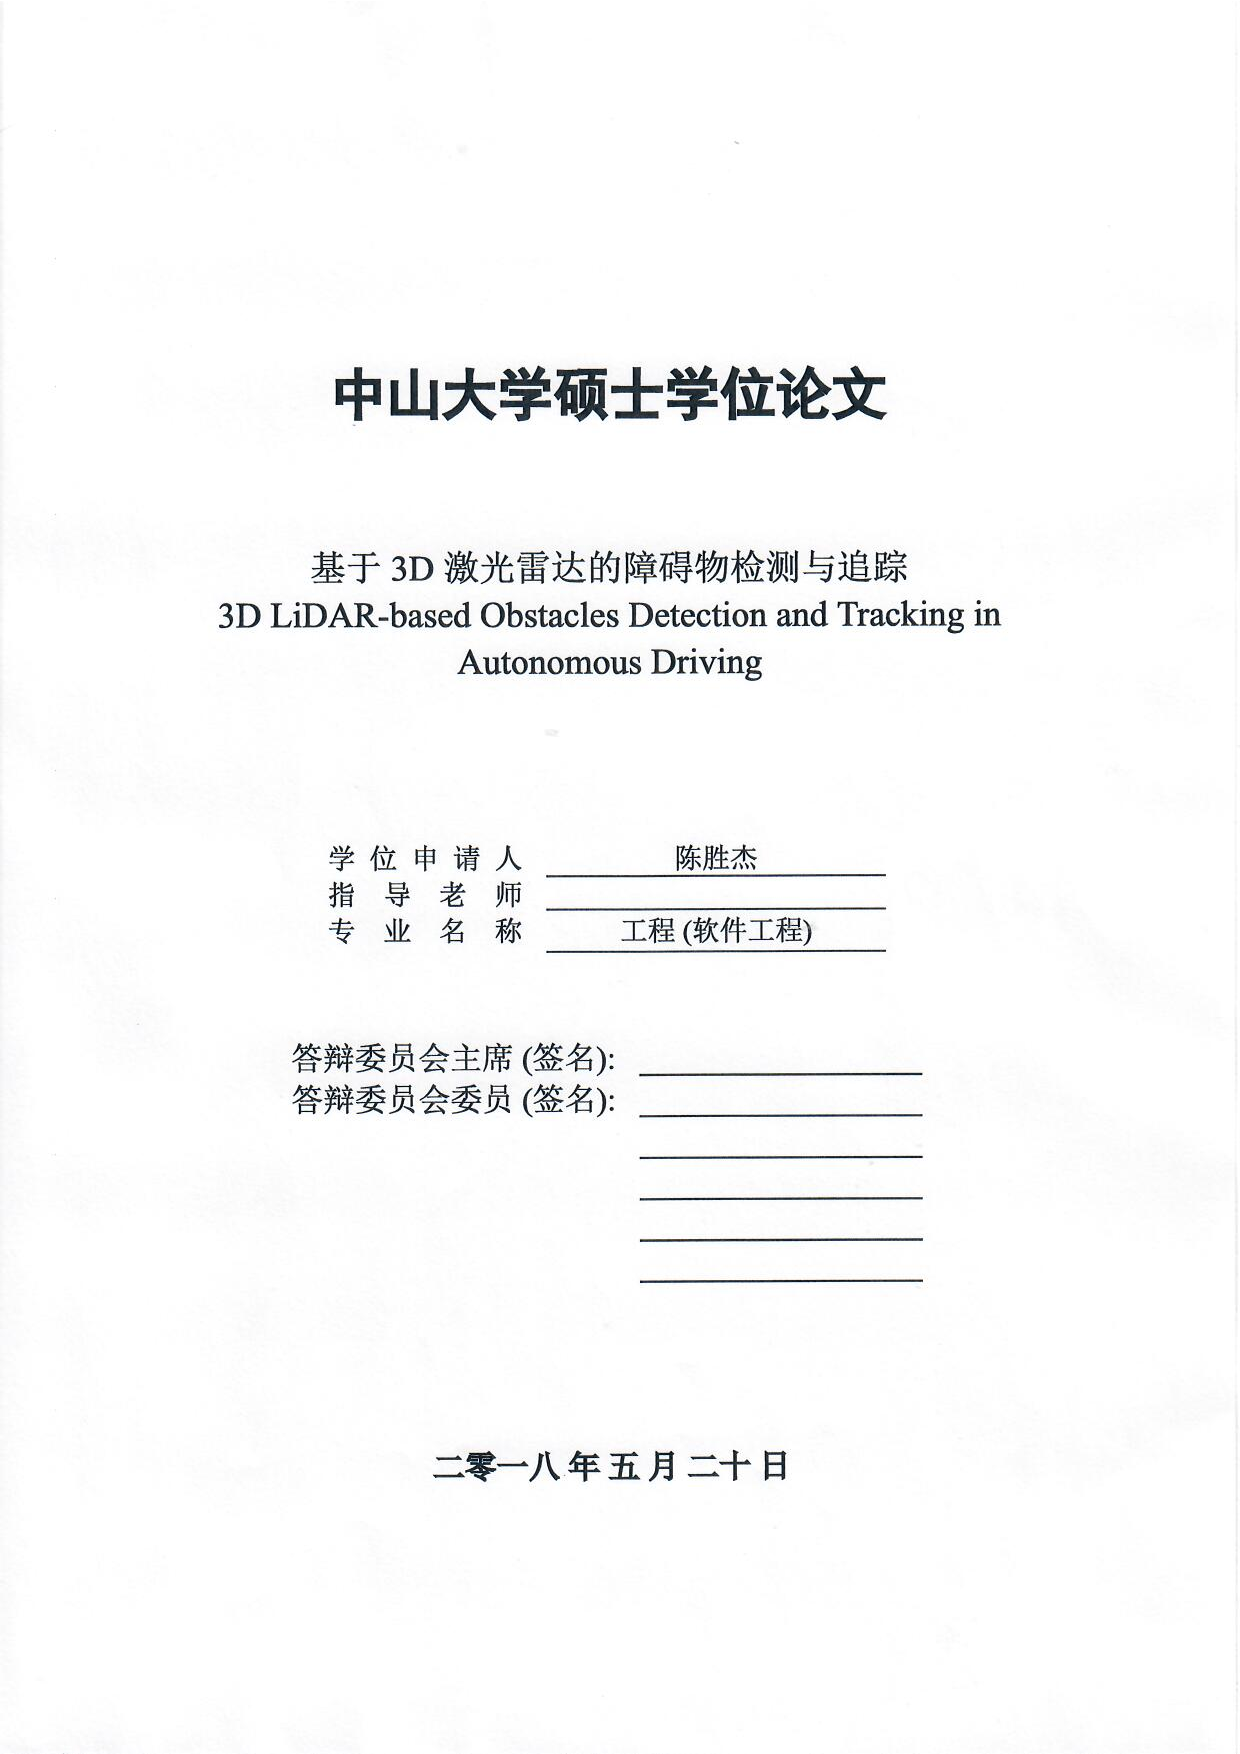
\includepdf{./signatures/TitlePage.pdf}
		\end{titlepage}	
	\else
		\begin{titlepage}
			\vspace*{31.5pt}
			\begin{center}
		
			\vspace*{21pt}
			\hei\chuhao{\textbf{中山大学硕士学位论文}}
		
			\vspace*{60pt}
			\song\xiaoer{\@ctitle}
		
			\xiaoer{\textrm{\@etitle}}
		
			\vspace*{80pt}
			\setlength{\@title@width}{6cm}	% 控制封面中下划线的长度。
			{\sihao\song{
			\begin{tabular}{lc}
			 学~~位~~申~~请~~人   &  \underline{\makebox[\@title@width][c]{\@cauthor}} \\
			 指~~~~导~~~~老~~~~师       &  \underline{\makebox[\@title@width][c]{\@csupervisor}} \\
			 专~~~~业~~~~名~~~~称 &  \underline{\makebox[\@title@width][c]{\@csubject}}\\
			\end{tabular}}
			}
		
			\vspace*{42pt}
			\setlength{\@title@width}{5cm}
			{\sanhao\song{
			\begin{tabular}{lc}
			 答辩委员会主席(签名):  &  \underline{\makebox[\@title@width][c]{~}} \\
			 答辩委员会委员(签名):  &  \underline{\makebox[\@title@width][c]{~}} \\
			 ~ &  \underline{\makebox[\@title@width][c]{~}}\\
			 ~ &  \underline{\makebox[\@title@width][c]{~}}\\
			 ~ &  \underline{\makebox[\@title@width][c]{~}}\\
			 ~ &  \underline{\makebox[\@title@width][c]{~}}\\
			\end{tabular}}	% 不加粗
			}
		
			\vspace*{60pt}
		
			\vspace*{21pt}
		
			\song\sanhao{\textbf{\@cdate}}
			\end{center}
		\end{titlepage}
	\fi
	
	\ifprint
		% 打印时插入空白页
		\newpage
		\thispagestyle{empty}
		\mbox{}
	\fi
	
	%%%%%%%%%%%%%%%%%%%   Originality Statement  %%%%%%%%%%%%%%%%%%%%%%%
	\clearpage
	\pdfbookmark[0]{论文原创性声明}{originality}
	
	\ifsubmit
		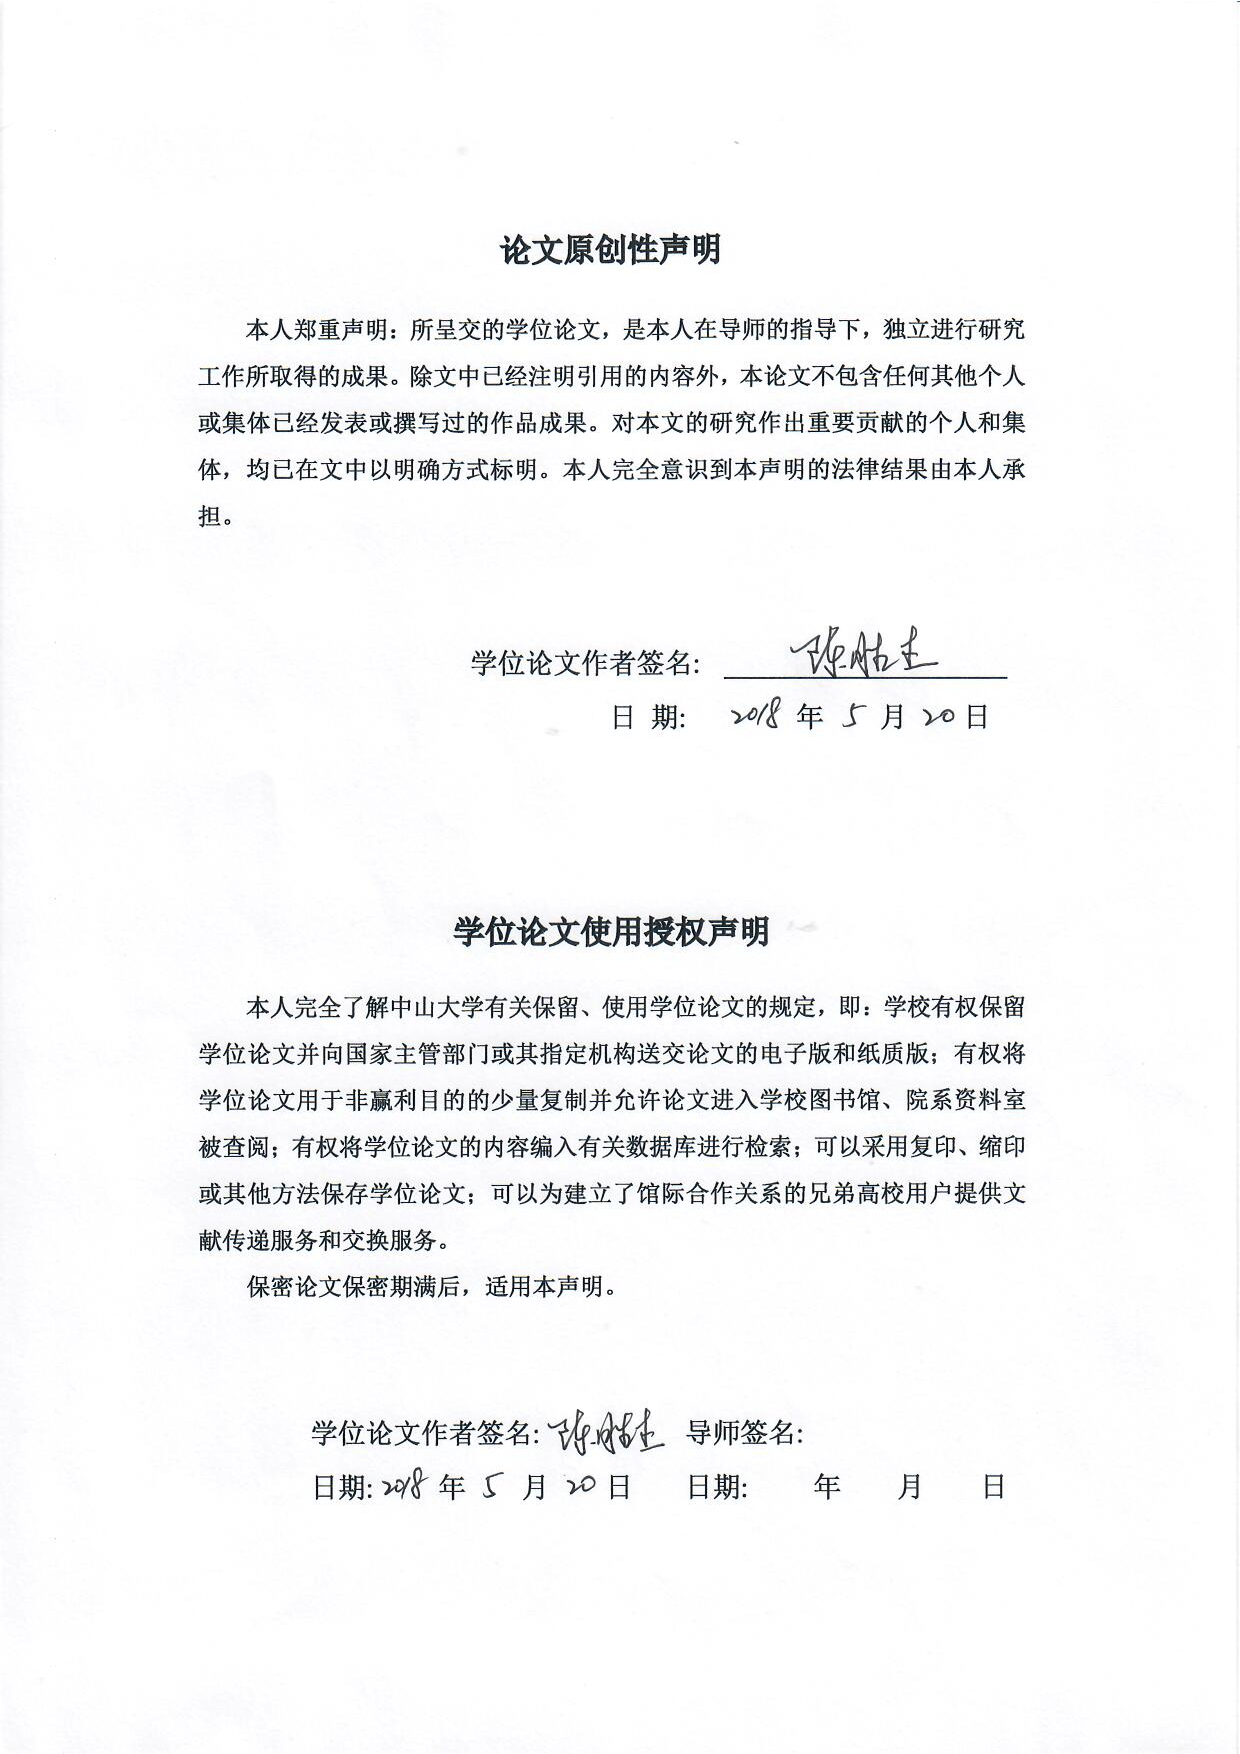
\includepdf{./signatures/OriginalityStatement.pdf}
	\else
		\chapter*{\centering\sanhao\song\bfseries 论文原创性声明}
		\song\defaultfont
		本人郑重声明:所呈交的学位论文,是本人在导师的指导下,独立进行研究工作所取得的成果。除文中已经注明引用的内容外,本论文不包含任何其他个人或集体已经发表或撰写过的作品成果。对本文的研究作出重要贡献的个人和集体,均已在文中以明确方式标明。本人完全意识到本声明的法律结果由本人承担。
		
		\vspace*{40pt}
		\begin{flushright}
		\setlength{\@title@width}{5cm}
		  {\sihao\song{
		  \begin{tabular}{lc}
		    学位论文作者签名:           &  \underline{\makebox[\@title@width][c]{~}} \\
		    \qquad\qquad~~~ 日~~期:  &  \qquad 年\qquad 月\qquad 日 \\
		  \end{tabular}}
		 }
		\end{flushright}
	
		%%%%%%%%%%%%%%%%%%%   Authorization Statement  %%%%%%%%%%%%%%%%%%%%%%%
		\vspace*{60pt}
		\pdfbookmark[0]{学位论文使用授权声明}{authorization}
		\begin{center}
		  \sanhao\song\bfseries{学位论文使用授权声明}
		\end{center}
		
		\song\defaultfont
		本人完全了解中山大学有关保留、使用学位论文的规定,即:学校有权保留学位论文并向国家主管部门或其指定机构送交论文的电子版和纸质版;有权将学位论文用于非赢利目的的少量复制并允许论文进入学校图书馆、院系资料室被查阅;有权将学位论文的内容编入有关数据库进行检索;可以采用复印、缩印或其他方法保存学位论文;可以为建立了馆际合作关系的兄弟高校用户提供文献传递服务和交换服务。
		
		保密论文保密期满后,适用本声明。
		
		\vspace*{40pt}
		\begin{flushright}
		\setlength{\@title@width}{5cm}
		  {\sihao\song{
		  \begin{tabular}{ll}
		    学位论文作者签名: \qquad\qquad\qquad  &  导师签名: \qquad\qquad\qquad\\
		    日期: \qquad 年\qquad 月\qquad 日     &  日期: \qquad 年\qquad 月\qquad 日 \\
		  \end{tabular}}
		 }
		\end{flushright}
	\fi

	\thispagestyle{empty}   % 去掉页码
	
	\ifprint
		% 空白页
		\newpage
		\thispagestyle{empty}
		\mbox{}
	\fi
	
	%%%%%%%%%%%%%%%%%%% Abstract and Keywords 摘要和关键词 %%%%%%%%%%%%%%%%%%%%%%%
	%中文摘要格式
	\clearpage
	\markboth{摘~要}{摘~要}
	\pdfbookmark[0]{摘~~要}{cabstract}
	
	% 摘要不加到目录中
	%\addcontentsline{toc}{chapter}{摘要}
	
	% 开始罗马数字编号
	\setcounter{page}{1}
	\pagenumbering{Roman}
	\thispagestyle{plain}
	
	\begin{flushleft}
	\setlength{\@title@width}{5cm}
	  {\xiaosi\song{
		\begin{tabular}{lcl}
		论文题目 & : & \@ctitle\\
		专业 & : & \@csubject \\
		硕士生 & : & \@cauthor \\
		指导老师 & : & \@csupervisor \\
		\end{tabular}}
	 }
	\end{flushleft}
	
	% 中文摘要:小二,黑体加粗,居中
	\begin{center}
	\xiaoer\hei\bfseries 摘\qquad 要
	\end{center}
	
	\vspace{\baselineskip} % 新增摘要后空行
	
	% 插入中文摘要
	\song\defaultfont
	\@cabstract
	\vspace{\baselineskip}
	
	\hangafter=1\hangindent=52.3pt\noindent
	{\hei\xiaosi 关键词:} \@ckeywords
	%\thispagestyle{empty}
	
	\ifprint
		% 空白页
		\newpage
		\thispagestyle{empty}
		\mbox{}
	\fi

	\clearpage
	% 避免空白页影响页码编号
	\pagenumbering{Roman}	
	\setcounter{page}{2}
	
	% 英文摘要格式
	\markboth{ABSTRACT}{ABSTRACT}
	\pdfbookmark[0]{ABSTRACT}{eabstract}
	
	% 英文摘要不加到目录中
	%\addcontentsline{toc}{chapter}{ABSTRACT}
	
	\thispagestyle{plain}
	
	% 如果英文title太长,手动分成两行
	\begin{flushleft}
	\setlength{\@title@width}{5cm}
		{\xiaosi{
		\begin{tabular}{ll}
		%Title: & \@etitle \\
		%		&		   \\
		Title: & \@etitle \\
		Major:      &  \@esubject \\
		Name:       &  \@eauthor \\
		Supervisor: &  \@esupervisor \\
		\end{tabular}}
		}
	\end{flushleft}
	
	% ABSTRACT三号居中
	\begin{center}
	\sanhao{\bf{ABSTRACT}}
	\end{center}
	\vspace{\baselineskip}
	
	% 插入英文摘要
	\@eabstract
	\vspace{\baselineskip}
	
	\hangafter=1\hangindent=60pt\noindent
	{\textbf{Keywords:}} \@ekeywords
	\thispagestyle{plain}

	\ifprint
		% 空白页
		\newpage
		\thispagestyle{empty}
		\mbox{}
	\fi
	
	% 避免空白页影响页码编号
	\clearpage
	\pagenumbering{Roman}
	\setcounter{page}{3}
	} % end of `\def\makecover`

	\def\maketime{
		% 如果需要加名字和日期(日期根据生成文档日期变更)
		\begin{flushright}
			\begin{tabular}{cl}
				\@cauthor & \\
				\@cdate &
			\end{tabular}
		\end{flushright}
	}
\makeatother

%%%%%%%%%%%% 脚注 %%%%%%%%%%%%%%%%%
% 脚注跨章单独编号
% 脚注跨章连续编号
%\counterwithout*{footnote}{chapter}
% 结合geometry布局进行调整
%\renewcommand\footnoterule{\flushleft\raisebox{20pt}{\rule{42.68pt}{0.4pt}}}
%\skip\footins=0.07pt
%\renewcommand\footnoterule{
%	\vspace*{1.5cm}
%	\hrule width 2.5cm
%	\vspace*{0.3cm}
%}
\renewcommand{\footnoterule}{%
	\kern 38pt
	% 尾注线属性
	\hrule width 2.5cm height 0.5pt
	% 尾注行距
	\kern 1pt
}

%\setlength{\skip\footins}{1cm} % gap between text and footer
%\setlength{\footskip}{1.5cm}
% 调整脚注行距
%\renewcommand\footnotesep{0in}
	
	% 定义所有的.eps/.pdf图片文件在figures子目录下
	\graphicspath{{figures/}}
	
	% ——————————————————————————————————————————————
	% 以下是论文导言部分,包括论文的封面,中英文摘要和中文目录(首页都是plain样式,无页眉)
	\frontmatter
	\fancypagestyle{plain}{
		\fancyhf{}
		\renewcommand{\headrulewidth}{0 pt}
		\fancyfoot[C]{\song\xiaowu~\thepage~}
	}
	
	%%%%%%%%%%   封面   %%%%%%%%%%
	% !Mode:: "TeX:UTF-8"

\cheading{中山大学硕士学位论文}      % 设置正文的页眉,需要填上对应的毕业年份
\ctitle{基于流数据的三维物体检测与追踪}    % 封面用论文标题,自己可手动断行
\etitle{3D Streaming-based Object Detection and Tracking}    %论文英文标题
\csubject{计算机科学与技术}   % 专业名称
\esubject{Computer Science and Technology}


\ifreview
	% 盲审时用
	\cauthor{ }            % 学生姓名
	\eauthor{ }
	\csupervisor{ }        % 导师姓名
	\esupervisor{ }
\else
	\cauthor{郭叙森}            % 学生姓名
	\eauthor{Guo Xusen}
	\csupervisor{黄凯~教授}        % 导师姓名,~用于间隔职称
	\esupervisor{Prof. Huang Kai}
\fi


% 自动数字日期
%\cdate{\the\year~年~\the\month~月~\the\day~日}
% 自动中文日期
%\cdate{\CJKnumber{\the\year}~年~\CJKnumber{\the\month}~月~\CJKnumber{\the\day}~日}
% 定制中文日期
%\cdate{二零二零~年~五~月~二十~日}
\cdate{二〇二〇~年~五~月~二十~日}

\cabstract{
近年来,随着深度学习技术的不断发展,三维物体检测领域取得了许多令人瞩目的成果,这些研究成果带动着众多自动驾驶创业公司蓬勃发展。然而,目前大多数三维物体检测方法都是针对单帧数据的,这些方法忽略了帧数据的时间连续性,无法利用帧与帧之间的时序信息,对检测算法的落地增加了不少难度。本工作旨在探索三维物体检测中时序信息的利用问题,通过深度学习技术去挖掘流数据的帧间相关性。为此,本文针对性地构建了一个基于关键帧的双路三维物体检测网络。该网络首先对关键帧进行物体检测,然后基于神经网络学习到的时序信息,将关键帧的检测结果传播到非关键帧。该传播过程可以将不同帧的同一物体关联,因此在得到检测结果之后,追踪结果也很容易获得,从而使得该网络同时具备三维物体检测与多目标追踪的能力。实验表明,本方法在速度与精度上都要优于同类型的单帧物体检测网络。在KITTI数据集的目标追踪比赛中,本方法在三维多目标追踪任务中取得了和当前最好方法相当的性能,分别取得了76.68\%的MOTA和81.65\%的MOTP。
}

\ckeywords{三维物体检测;多目标追踪;时序信息;关键帧}

\eabstract{
Recent approaches for 3D object detection have made tremendous progresses due to the development of deep learning. However, previous researches for detection are mostly based on individual frames, leading to limited exploitation of information between frames. In this paper, we attempt to leverage the temporal information in streaming data and explore 3D streaming based object detection as well as tracking. Toward
this goal, we set up a dual-way network for 3D object detection based on key frames, then propagate predictions to non-key frames through a motion based interpolation algorithm guided by temporal information. Our framework is not only shown to have significant improvements on object detection compared with frame-by-frame paradigm, but also proven to produce competitive results on KITTI Object Tracking Benchmark, with
76.68\% in MOTA and 81.65\% in MOTP respectively.
}

\ekeywords{3D object detection; Multiple object tracking; Temporal information; Key frame}

\makecover

\clearpage

	
	%%%%%%%%%%   目录   %%%%%%%%%%
	% 单独从 1 开始编页码
	%\clearpage{\pagestyle{empty}\cleardoublepage}
	%\setcounter{page}{1}
	%\pagenumbering{arabic}
	
	% 设置目录两字的格式
	\titleformat{\chapter}{\centering\sanhao\hei}{123}{}{}[]
	\pdfbookmark[0]{目~~录}{mulu}
	
	% 设置目录页无页眉,页脚为居中页码
	\pagestyle{plain}
	% 中文目录
	\tableofcontents
	
	\clearpage
	\pagestyle{newfancy}
	% ——————————————————————————————————————————————
	% 以下是论文正文,内容在body子文件夹下
	% 默认即开章页无页眉
	\mainmatter\defaultfont\sloppy\raggedbottom
	% 设置开章页页眉页脚样式
	\makeatletter
	\fancypagestyle{plain}{
		\fancyhf{}
		\fancyhead[C]{\song\wuhao \@cheading}            % 首页页眉格式
		\fancyfoot[C]{\song\xiaowu ~\thepage~}           % 首页页脚格式
		\renewcommand{\headrulewidth}{0.5pt}
		\renewcommand{\footrulewidth}{0pt}}
	\makeatother
	% 单独从1开始编页码
	\setcounter{page}{1}
	% chapter标题格式:小二,黑体,居中
	\titleformat{\chapter}{\centering\xiaoer\hei}{}{5em}{\chaptername \qquad}
	
	%%%%%%%%%%   正文   %%%%%%%%%%
	% !Mode:: "TeX:UTF-8"
\chapter{引言}
\label{ch:intro}
本章主要介绍了自动驾驶的技术背景以及三维物体检测在自动驾驶技术中的重要作用,然后引出了目前三维物体检测技术的局限性。之后,本章介绍了目前国内外对三维物体检测的研究进展,也简单介绍了三维多目标追踪的研究进展。最后,本章简要概括了本文的工作重点以及技术创新要点,强调了本文研究对于自动驾驶领域的重要意义。

\section{研究背景与意义}
\label{sec:background}
近几年来, 深度学习的迅猛发展赋予了机器越来越强的智能。在计算机视觉、自然语言处理等领域的某些任务上,机器甚至能够表现出比人类更好的性能\cite{he2016deep,DevlinBERT}。 在这样的大背景下, 无人驾驶(Autonomous Driving) 作为最能够体现机器智能的应用场景之一,受到了学术界和工业界的广泛关注。 无人驾驶要求机器能够像人类一样识别道路场景,包括行人和车辆的状态以及车道线等,并且能够根据这些信息高效地进行路径规划来实现与人类类似的驾驶行为。 无人驾驶应用十分广泛,无论是民用还是军工领域。 机器取代人类驾驶车辆,一方面能让人们出行效率更高, 另一方面,机器之间的通讯比人类效率更高,这使得车辆能够更好的规划自己的行驶路径,降低交通事故发生概率。作为智慧城市的不可缺少的组成部分, 无人驾驶也能在非常时期发挥重要作用。譬如在面对重大传染病时(如2019年末爆发的COVID-19),人员之间要尽量减少接触,此时无人驾驶能在保证安全的情况下,极大方便人们的日常生活,包括出行以及货物配送。因此,无人驾驶作为可预见的未来技术,一直是各国在高科技领域的“必争之地”。近十几年来,国内外的无人驾驶平台如雨后春笋般冒出,既有老牌互联网大公司开展的新业务,如国内百度的Apollo\footnote[1]{http://apollo.auto/}(如\figurename \ref{fig:apollo}),美国Google的Waymo\footnote[2]{https://waymo.com/}(如\figurename \ref{fig:waymo})等;也有新型汽车行业巨头,如Uber、特斯拉、滴滴、上汽等;另外,还有新兴的无人驾驶创业公司,如pony.ai、图森未来、驭势科技等。这些都是推动无人驾驶商业化不可忽视的力量,也是推动无人驾驶技术落地的中坚力量。

\begin{figure}[!t]
	\centering
	\begin{minipage}[t]{0.40\textwidth}
		\centering
		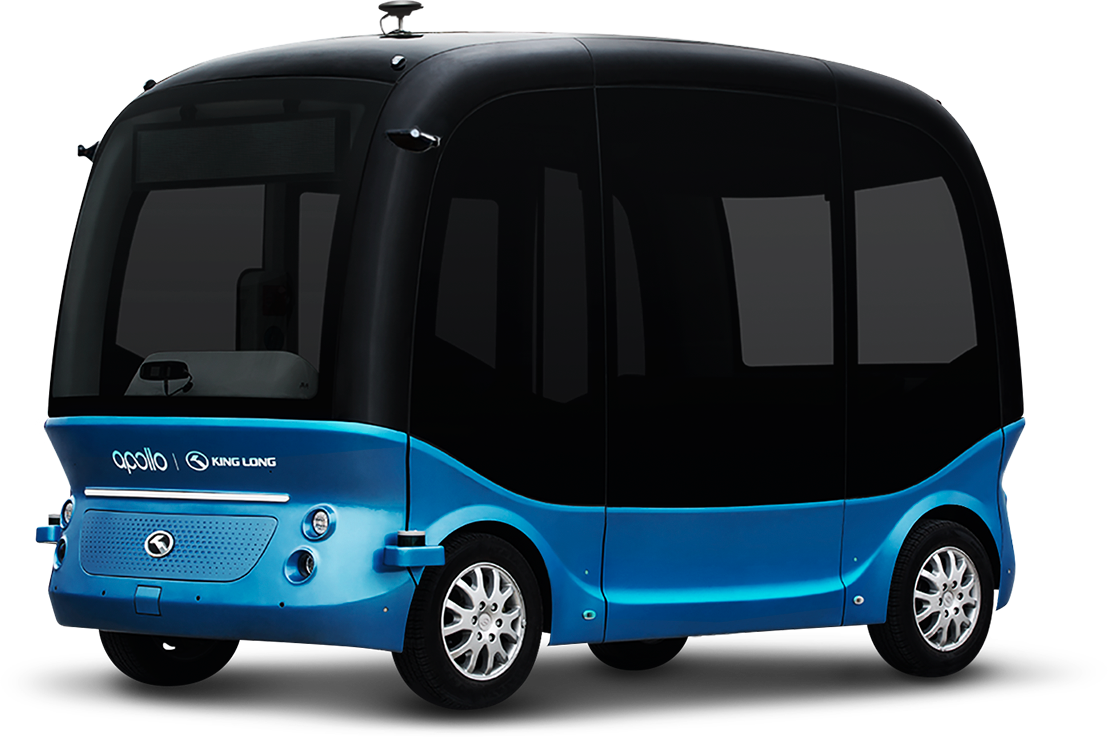
\includegraphics[width=\textwidth]{./imgs/apollo.png}
		\caption{Apollo自动驾驶汽车}
		\label{fig:apollo}
	\end{minipage}
	\begin{minipage}[t]{0.55\textwidth}
		\centering
		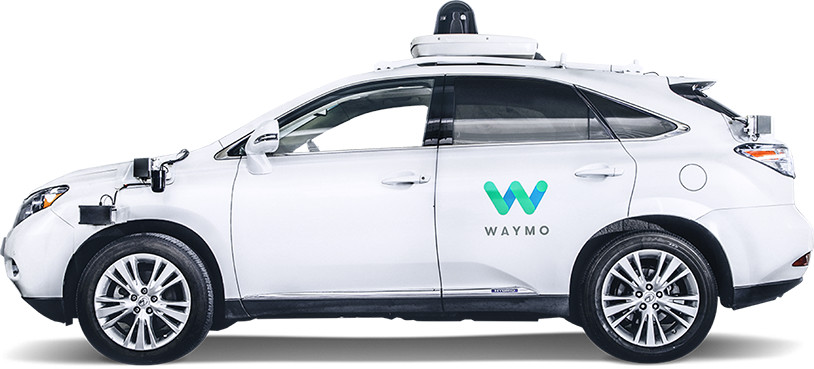
\includegraphics[width=\textwidth]{./imgs/waymo.jpg}
		\caption{Waymo自动驾驶汽车}
		\label{fig:waymo}
	\end{minipage}
\end{figure}


无人驾驶技术主要包括感知、决策和规划三个重要模块,其中感知模块是无人驾驶技术的基础,也是难点。感知模块的任务是赋予机器理解环境的能力,使机器能够准确捕获复杂道路场景的有用信息。目前无人驾驶车辆依赖多种传感器感知环境, 譬如激光雷达(LIDAR)、摄像头、毫米波雷达等。这些传感器都有着各自的优缺点,特别是在价格、使用场景以及探测距离方面,如表\ref{table:sensor_cmp}所示。因此,目前绝大多数自动驾驶公司在感知模块都使用多传感器融合技术,让各传感器优劣互补。多传感器采集的数据会通过算法进行融合,尽可能准确的还原真实的三维环境信息,以便用于后续的目标检测以及跟踪等任务。

环境感知中一大核心任务是物体检测(Object Detection), 即通过分析传感器采集的数据,确定环境中各目标的位姿,包括其在世界坐标系下的坐标、形状信息以及朝向。不同于以图像为主要数据载体的二维物体检测,自动驾驶领域的物体检测任务要求预测目标在三维空间的位姿信息,即三维目标检测。三维目标检测比二维目标检测更加具有挑战性,这是因为维度诅咒(the curse of dimensionality)的存在: 当维度增加时,空间的体积增加的非常之快(以指数增加),以致于可用的数据变得稀疏。 三维物体检测的一大挑战,就是三维数据的稀疏性。目前无人驾驶中三维数据的获得主要是依靠激光雷达,其原理是通过高速旋转的激光发射器向周围发射激光,然后检测接收到反射回来光线的时间间隔来计算反射点的距离。激光雷达的线束对其分辨率有很大影响,特别是对于远距离的目标,在低线束(例如16线)激光雷达中可能只有稀疏的几个点,完全无法分辨。而分辨率高的高线束的激光雷达则十分昂贵,以 Velodyne 64线激光雷达为例,其价格高达十几万美金,因此多数无人驾驶技术方案都需要在激光雷达分辨率与价格之间做出权衡。最近一种非完全旋转的激光雷达——固态激光雷达\footnote[3]{http://www.robosense.cn/rslidar/rs-lidar-m1}受到越来越多人的关注,它们具备数据采集速度快、分辨率高、价格低廉以及环境适应性强等特点,被自动驾驶行业给予厚望。然而目前该技术尚不成熟,还没经过广泛的实际场景检验,离落地还有一段时间,因此暂时不在各大方案的候选传感器之内。短期来看,传统的机械式激光雷达仍是各大自动驾驶平台的首选。

\begin{table}
	\centering
	\wuhao
	\caption{自动驾驶各传感器对比\cite{FirstAVbook}。}
	\vspace{0.3cm}
	\resizebox{\textwidth}{!}{
		\begin{tabular}{cccccccc}
			\toprule[1.5pt]
			传感器    & 激光雷达(LIDAR) & 摄像头(Camera) & 毫米波雷达 \\ \midrule
			外形      & \begin{minipage}{0.13\textwidth}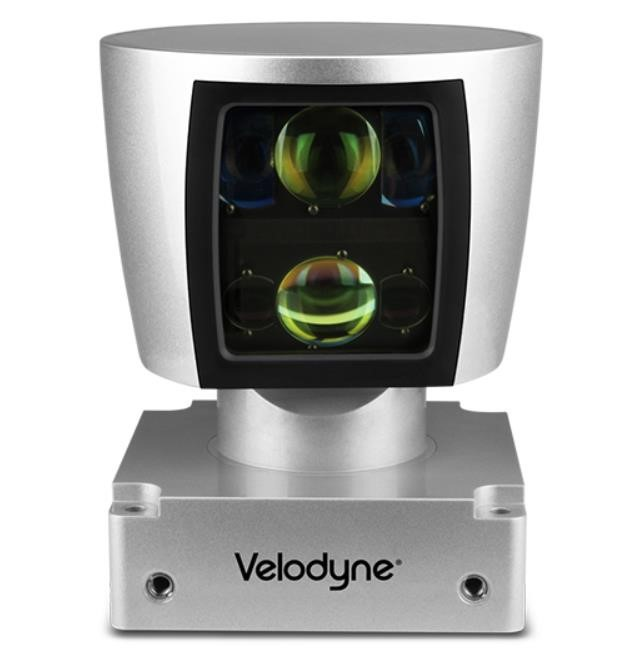
\includegraphics[width=\linewidth]{../figures/imgs/lidar.jpg}\end{minipage} & \begin{minipage}{0.15\textwidth}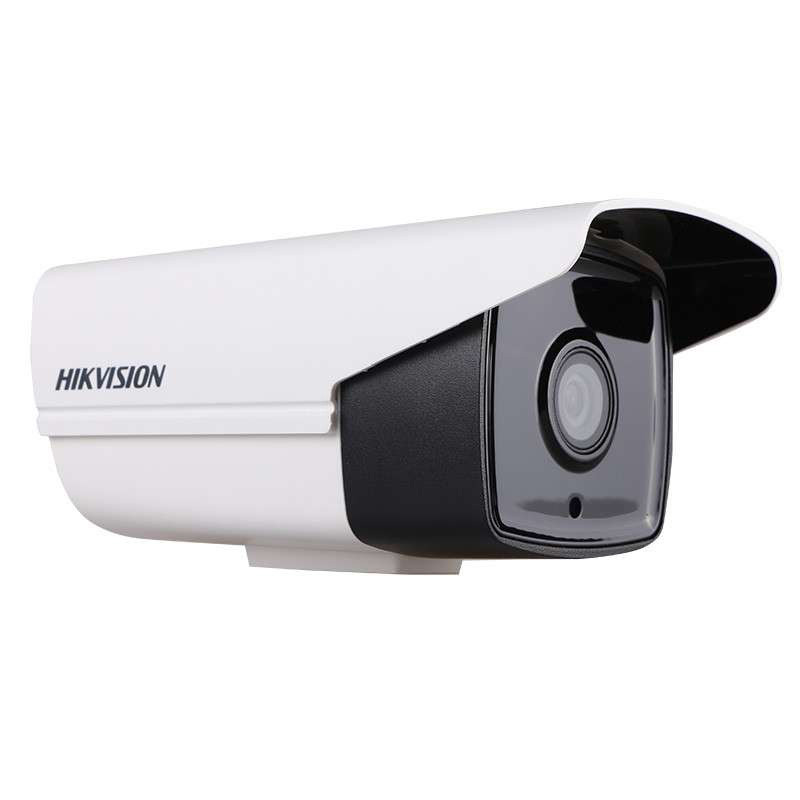
\includegraphics[width=\linewidth]{../figures/imgs/camera.jpg}\end{minipage} & \begin{minipage}{0.15\textwidth}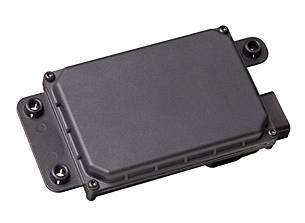
\includegraphics[width=\linewidth]{../figures/imgs/mlidar.jpeg}\end{minipage} \\ \hline
			价格      & 8000美元以上    & 35-50美元         & 300-500美元    \\ \hline
			优点      & \makecell*[c]{扫描周围环境得到精确\\环境信息、距离信息}   & \makecell*[c]{成本比较低,通过算法\\可以实现各种功能} & \makecell*[c]{不受天气影响,\\测量精度高}  \\ \hline
			缺点      & \makecell*[c]{成本高,大雾、雨雪天气\\效果差,无法图像识别}  & \makecell*[c]{恶劣环境下失效,难以测距,\\探测距离较近,算法要求高}   & \makecell*[c]{无法识别道路指示牌,\\无法识别行人}   \\ 
			\bottomrule[1.5pt]
	\end{tabular}}
	\label{table:sensor_cmp}
\end{table}


根据使用传感器数据的不同,目前三维物体检测的研究主要有三个方向:基于图像数据的方案\cite{7780605, chen20183d},基于点云数据的方案\cite{li20173d,engelcke2017vote3deep,zhou2018voxelnet,simon2018complex,shi2019pointrcnn},以及基于多传感器数据融合的方案\cite{qi2018frustum,chen2017multi,ku2018joint}。借助深度学习技术,这些方案都取得了很不错的结果。尽管如此,目前基本所有的三维物体检测方案都是针对单帧数据进行检测。对于真实的自动驾驶场景的物体检测任务来说,数据都是以流的形式连续获取的。从算法落地的难易程度方面考虑,开发针对流数据的三维物体检测算法相比于基于单帧的三维物体检查算法更加具有优势。相比于单帧数据,流数据可以提供同一目标在一段时间内的连续信息。一方面,由于检测噪声(误检测的物体)在时间维度上连续性较差,因此时序上的连续信息有利于检测算法筛除误检测的目标。另一方面,对于遮挡以及物体框被边界截断的目标,在流数据中可以利用前后帧的信息对其进行补全,从而获得更好的检测性能,这对于基于单帧的检测算法来说是难以实现的。最后值得注意的是,流数据一般有很强的数据冗余性,即相邻帧之间绝大多数信息都相同,只有存在物体运动的区域才会有些许差异。对于流数据物体检测,如果使用基于单帧的物体检测算法,则需要逐帧进行检测,然后再将结果关联,这个过程会存在很多重复计算的过程,十分耗时。但是如果使用基于流数据的物体检测算法,则有可能只对少量帧(例如关键帧)进行检测,然后利用流数据的冗余性与时序信息将检测结果传播到其余帧,从而能够更为高效的完成三维物体检测任务。 因此,将基于单帧的三维物体检测算法扩展到流数据场景,能显著提高三维物体检测算法的准确率与效率,也是将三维物体检测技术落实到实际场景的必经之路,具有很强的实践意义。本工作旨在探索基于关键帧的三维流数据物体检测框架,同时也探究了三维时序信息的特征编码以及预测框的传播算法,为后续三维目标检测算法的落地工作提供一个可行的参考方案。

\section{国内外研究进展}
\label{sec:realted_work}
目前国内外针对流数据的三维物体检测研究还较少,而基于单帧数据的三维物体检测以及基于视频流的二维物体检测的研究较为丰富。 因此,本节将简要概述三维物体检测以及视频流物体检测的前沿进展,并分析这些方法的优缺点。另外,本节也将简要介绍三维场景的多目标跟踪的前沿进展,为本工作中多目标跟踪部分提供参考。

\subsection{三维物体检测}
\label{3d_detect}
目前大多数三维物体检测研究可以归类为三大方向:基于图像数据的方案,基于点云数据的方案,以及基于多传感器数据融合的方案,如\figurename \ref{fig:det_algo}所示。基于图像数据的方案中,又可分为基于单目相机数据、基于双目相机数据的三维目标检测;而基于点云数据的方案中根据点云数据的特征提取方式不同又可分为基于点的(Point-based)、基于体素的(Voxel-based)以及基于投影的(Projection-based),这些方法都将在本小节详细介绍。

\begin{figure}[h]
	%\vspace{-0.3cm}
	\begin{center}
		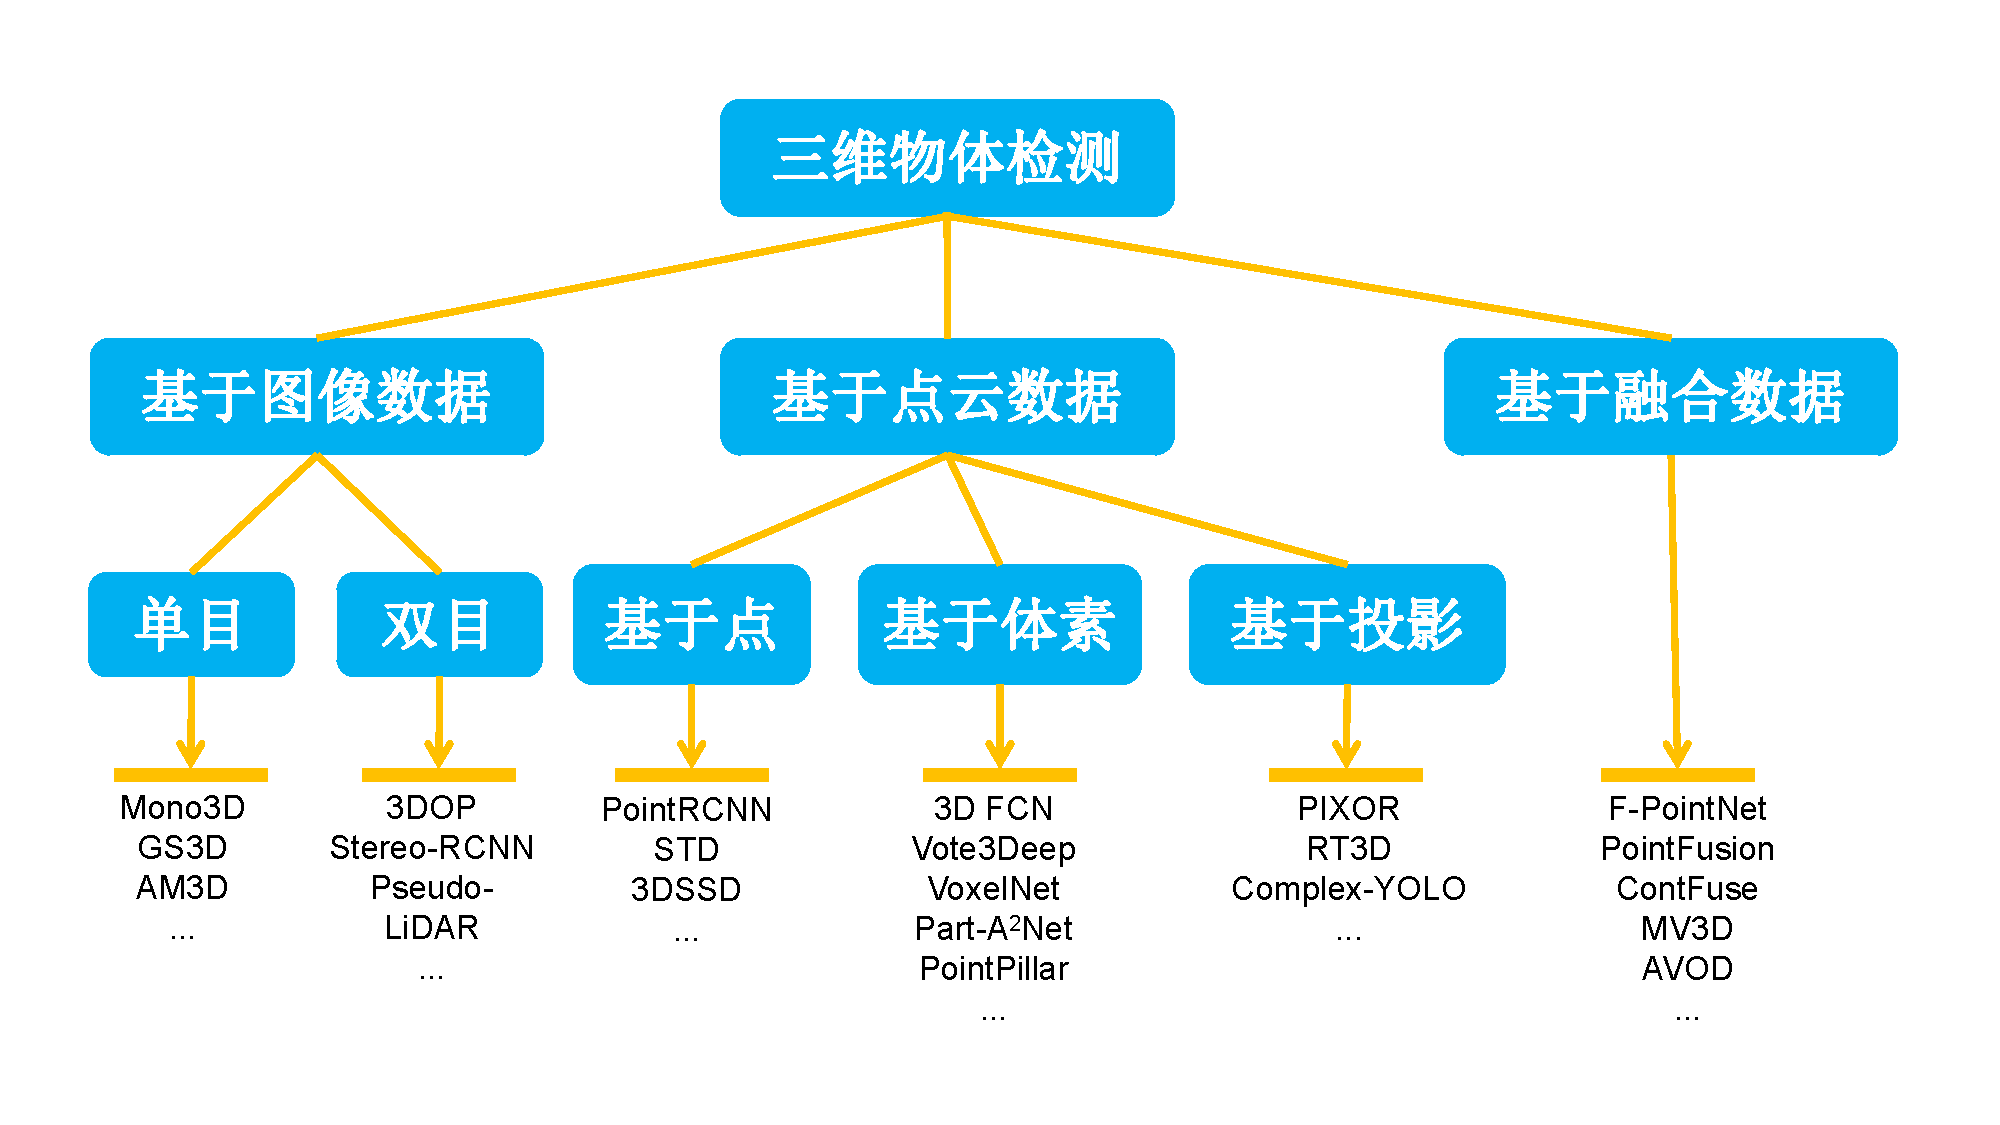
\includegraphics[trim={1.5cm, 1.5cm, 1.5cm, 1.5cm}, clip, width=\textwidth]{imgs/det_algo.pdf}
	\end{center}
	\vspace{-0.8cm}
	\caption{三维物体检测方法分类。}
	\label{fig:det_algo}
\end{figure}


\subsubsection{基于图像数据的三维物体检测}

基于图像数据的三维物体检测有两大类,一类是使用单目摄像头数据,另一类是使用多目(一般为双目)摄像头数据。对于单目摄像头数据,由于摄影几何学的限制,只凭一幅图像是无法恢复出像素点的三维信息的,也无法获得物体的真实的尺寸信息。然而对于特定类型的物体是有可能的,这是因为特定类型的目标往往具有很强的先验信息。这些信息可以被用来构建目标的几何模型,从而使三维物体检测能够顺利进行。对于单目图像三维物体检测,目前有基于目标几何约束提取3D候选框然后将其投影到图像平面提取特征进行预测的,如Mono3D \cite{7780605};也有先对图像进行二维目标检测得到二维边界框,然后利用先验信息对车辆的3D位姿进行建模,从而得到车辆的三维边界框,如\cite{Mousavian3D}以及GS3D\cite{li2019gs3d};另外也有工作使用现有2D物体检测框架以及深度图预测网络得到2D边界框和深度图像,然后再根据相机参数将深度图转换为三维点云,然后利用2D边界框对点云进行分割,最后嵌入RGB信息并使用PointNet\cite{qi2017pointnet}回归出三维边界框,如AM3D\cite{ma2019accurate}。然而,使用单张图像毕竟无法很好地获得物体三维信息,因此这类方法需要人工设计的几何特征来表征物体的深度信息。虽然数据采集简单,速度快,但是检测精度差,落地难。

双目摄像头从生物学上来说很接近人类的双眼视觉系统。对于双目摄像头数据,可以进行双目立体视觉匹配,通过相机之间的相对位置信息可以得到像素点的深度,从而可以在一定程度上恢复物体的三维信息。双目视觉相比于单目视觉有着更强的空间约束关系,因此结合场景先验,可以得到比单目相机更准确的三维物体检测结果。例如,对于两幅成对的图像,3DOP\cite{chen20183d}首先采用了Yamaguchi的方法\cite{Yamaguchi2014Efficient}计算每个像素的深度,生成点云数据,然后采用Struct-SVM\footnote{http://www.cs.cornell.edu/people/tj/svm\_light/svm\_struct.html}优化方法\cite{structSVM}提取3D候选框,最后采用与Fast-RCNN\cite{girshick2015fast}类似框架对3D候选框进行判别和回归,得到最终的预测框。Stereo RCNN\cite{licvpr2019}则将Faster-RCNN\cite{ren2015faster}网络扩展到双目立体视觉,将左右图像输入两个相同的候选框提取网络,然后通过自动对齐学习计算出左右视图中匹配的候选框,最后通过稠密匹配优化得到最终的三维检测结果。此外,还有工作使用双目相机数据生成伪激光雷达数据,然后使用这些点云数据进行三维物体检测。伪激光雷达数据的生成一般使用的是DRON\cite{DRON}或PSMNET\cite{chang2018pyramid}等深度估计网络,这类方法的代表是Pseudo-LiDAR\cite{Wang_2019_CVPR,you2020pseudolidar}。不过双目视觉对于远处的像素点深度估计非常不准,并且存在盲区,因此基于双目视觉的三维物体检测方案存在自身的理论缺陷,只能依靠神经网络根据先验信息弥补系统误差。

\subsubsection{基于点云数据的三维物体检测}

基于点云数据的方案是三维物体检测的主流方向,根据点云数据的特征提取方式不同这些方法又可分为Point-based、Voxel-based 以及Projection-based,本小节将详细介绍这三类方法。

Point-based的方法是直接在点云中提取特征,可以使用PointNet\cite{qi2017pointnet}, PointNet++\cite{qi2017pointnet++}, PointCNN\cite{PointCNN}, PointSIFT\cite{JiangPointSIFT}, Octnet\cite{RieglerOctNet}, Dynamic Graph CNN\cite{WangDynamic}等方法提取点的特征。Point-based的方法中比较有代表性的是香港中文大学提出的PointRCNN\cite{shi2019pointrcnn}以及其后续工作STD\cite{std2019yang}和3DSSD\cite{yang3DSSD20}。PointRCNN方法分为两步,第一步是将整个场景的点云分割为前景点和背景点,然后以自下而上的方式生成高质量候选框;第二步是将每个候选框进行坐标规范化,以便更好的学习局部空间特征然后生成更精确的边界框。STD在此基础上提出了一种基于球形锚点框的点云候选区域提取网络,然后引入了新的点池化层将候选区域内部点的特征从稀疏表达转化为稠密表达。相比于PointRCNN,STD具有更高的召回率以及更少的计算量。3DSSD是同一个研究团队提出的更加轻量型的单阶段三维物体检测网络,该网络提出了一种新的融合采样策略替代之前的上采样层,能够在准确率和速度上达到很好的平衡。这些方法在点云特征提取上都借鉴了PointNet++的思想,特别是使用\textit{set abstraction}操作在点云特征提取中引入可变的感受野。

Voxel-based的方法使用三维体素网格编码点云特征, 每个体素立方体的值由该立方体内的点决定,从而将不规则的三维点云数据编码成规则的三维体素数据, 便于后续使用神经网络进行特征提取。 这方面的代表工作有 3D FCN \cite{li20173d}、Vote3Deep \cite{engelcke2017vote3deep}、 VoxelNet \cite{zhou2018voxelnet}、Part-$A^2$Net\cite{shi2020part}以及PointPillar\cite{lang2018pointpillars}等。3D FCN和Vote3Deep直接对网格化的点云数据使用3D卷积提取特征,由于点云非常稀疏并且3D卷积需要在三个维度上操作,因此整个检测、定位的过程极其耗时。此外,受到感受野的影响,传统的3D CNN并不能很好的学习不同尺度的局部特征。VoxelNet只对非空的网格进行特征提取,并且使用多尺度结构学习不同尺度的信息,一定程度上弥补了这类方法的劣势。Part-$A^2$Net直接引用了VoxelNet的体素化方法,使用了稀疏卷积以及子流型稀疏卷积(Submanifold Sparse Convolution\cite{Graham3D})提取点云特征。PointPillar则是提出新型的垂直柱体网格化方法编码点云特征,使得编码速度更快。这类方法的一大缺点是体素大小不好确定,太大的话信息损失严重,太小则会造成巨大的计算量。 

Projection-based的方法是将点云在高度方向进行投影,将三维数据降维成二维的俯视图(BEV, bird eye view)数据。 考虑到在驾驶场景中, 道路基本是共面且水平的,因此在高度方向上投影对物体的位姿信息基本没有损失。 经过投影操作后,就能直接使用二维图像物体检测的方法进行物体检测。 PIXOR \cite{yang2018pixor}、RT3D\cite{8403277} 以及 Complex-YOLO \cite{simon2018complex,Simon_2019_CVPR_Workshops} 等属于这类方法,这些方法主要不同点在于点云的投影视角以及投影方式。 虽然降维能够带来速度的极大提升,然而由于点云数据的稀疏性,经过投影后目标的特征点损失很严重。 特征点的不足会很大程度上影响检测结果的准确性,特别是对于远处的目标以及小目标。

\subsubsection{基于多传感器数据融合的三维物体检测}

点云的稀疏性以及图像缺少深度信息都限制着相应方法的性能,一个自然而然的想法就是将这两种数据融合, 从而达到更好的检测性能。 基于多传感器融合的方法通过算法融合点云数据以及图像数据,从而提升三维物体检测的准确率。 这类方法的代表有 F-PointNet \cite{qi2018frustum}、PointFusion\cite{XuPointFusion}、ContFuse\cite{Ming2018Deep}以及 MV3D \cite{chen2017multi}、AVOD \cite{ku2018joint}等。 这些方法的区别主要在于数据融合的方式不同, F-PointNet首先使用二维物体检测方法检测出图像中的所有物体,之后对于每个物体,将其反投影回点云中得到一个视锥区域,之后使用PointNet++\cite{qi2017pointnet++}对该区域内的点进行分割,最后进行框回归。该方法通过先在图像中找出目标的大致区域,从而减少了算法在点云空间的搜索空间。然而,该算法的准确率受二维物体检测精度影响很大,在第一步没有检测出的物体,之后没有其他办法弥补。 PointFusion和ContFuse都是先分别在图像与点云数据中使用网络提取特征,然后将这两类特征进行融合并实现三维物体检测。MV3D 则是将二维物体检测中的区域提取网络扩展到三维空间, 提出了三维特征提取网络分别提取点云以及图像特征, 然后通过一个特征融合模块得到多视角融合特征,最后基于融合特征进行三维物体检测。 AVOD 在 MV3D 的基础上改进了特征提取模块, 引入了编码器-解码器结构从而能够得到全分辨率的特征图, 重点提升了小物体的定位精度。 本文工作中的检测模块是在AVOD框架的基础上进行改进的,使其能支持多帧输入,并引入了时序信息处理模块融合连续帧信息。

\subsection{视频流物体检测}
\label{video_detect}
视频流物体检测与单帧物体检测的主要区别在于是否利用了时序信息。 对于视频流物体检测,时序信息是物体的位姿在时间上的连续性的抽象体现。 目前,大多数视频流物体检测方法都是在两个层面利用时序信息,特征提取层面以及最终的框回归层面。 对于特征处理层面, 一般是根据运动信息将前后帧的的特征整合到关键帧,以增加关键帧的物体特征。 这个过程中需要使用到光流信息,即图像中各像素点的运动方向。 代表有 FGFA \cite{zhu2017flow}系列工作。 一般来说光流信息的获取比较困难,这也是限制该方法进一步发展的主要障碍。 对于在框回归层面利用时序信息,主要的工作有 T-CNN \cite{kang2018t, kang2016object} 与 Seq-NMS \cite{han2016seq}等。 T-CNN 使用预先计算的光流信息将关键帧的检测结果传播到临近帧,而 Seq-NMS 则是通过整合连续几帧的高置信度的候选框来提升目标检测中非极大值抑制(Non-Maximum Suppression,NMS)算法的性能。 最近, 也有一些工作试图通过神经网络学习连续帧之间的的时序信息, 从而避免使用高代价的光流数据。 这类方法的代表有 D\&T \cite{feichtenhofer2017detect}。 D\&T 提出了一个双路目标检测网络,可以同时时间视频流的目标检测以及目标追踪。 该网络可以输入多帧数据进行检测, 并且通过互相关操作(Cross-correlation) 来学习相邻帧之间相同物体的对应关系以及偏移。 本文的算法框架在一定程度上也借鉴了 D\&T 的结构, 不过我们在他的基础上进行了很大的改进,使其能够适应三维物体的流数据检测。

\subsection{三维多目标追踪}
\label{tracking}
目前基本上所有的三维多目标追踪方法都是先对流数据的每一帧进行目标检测,然后再将这些检测框关联起来, 这种范式也被称为 \textit{Tracking by Detection} \cite{lenz2015followme}。 三维多目标追踪的工作有很多,比较有代表性的有 FaF \cite{luo2018fast}, 3D-CNN/PMBM \cite{scheidegger2018mono}以及 DSM \cite{frossard2018end}等。 FaF 使用首先将点云流数据结构化成四维张量,然后构建了一个简单的特征提取网络提取特征,最后使用不同的网络头分别预测得到三维目标检测,多目标追踪以及运动方向预测结果。该方法能够整合前 $n$ 帧的检测结果得到精确的物体运动轨迹。 然而该方法计算量巨大, 并且网络参数调节需要有很高的技巧。  3D-CNN/PMBM 首先构建神经网络从单张图像预测物体的三维位姿, 然后将所有帧的检测框送入泊松多重伯努利 (Poisson Multi-Bernoulli Mixture, PMBM) 混合追踪滤波器进行滤波,得到最终的三维多目标追踪结果。 该方法只使用单帧图像进行三维目标检测,效果有限。 DSM 首先使用单帧三维物体检测框架 MV3D \cite{chen2017multi} 对每一帧数据进行物体检测得到三维检测框, 然后通过一个匹配网络(\textit{Matching net})以及得分网络(\textit{Scoring net})关联所有的检测框。 该方法需要对每一帧数据都进行检测, 并且帧与帧之间的时序信息基本上没有被使用,因此不是针对流数据的高效方法。

\section{本文工作及创新点}
\label{subsec:contribution}
本文提出了一个双路物体检测与追踪(\textbf{D}ual-way \textbf{O}bject \textbf{D}etection and \textbf{T}racking, \textbf{DODT})框架, 实现了流数据场景的高效三维物体检测与追踪。 本框架的构建是基于以下几个观察: (1) 点云能够与图像融合从而丰富物体的视觉特征, 这点在 \cite{chen2017multi,ku2018joint}中得到了证实; (2) 除了通过光流数据, 时序信息也能够通过计算相邻帧间的互相关信息,这点通过 D\&T\cite{feichtenhofer2017detect} 也能够得到验证; (3) 特征在连续帧之间的变化是连续的, 我们可以只对关键帧进行检测,然后将结果传播到非关键帧, 这样可以极大的减少计算量。 对于第一点, 本文借用了 AVOD\cite{ku2018joint} 中的数据融合方案,将点云数据提供的 BEV 信息与图像融合。 对于第二点, 本文构建了一个时序模块(Temporal module), 该模块使用互相光操作在 BEV 空间中计算相邻关键帧的时序特征, 然后预测相同物体在不同关键帧中同时出现的概率以及偏移量。 与 \cite{feichtenhofer2017detect,dosovitskiy2015flownet} 不同的是, 本模块的互相关操作是在后候选框层面进行的,不需要全局计算, 这极大地提高了模块的运行效率。 对于最后一点, 我们将 DODT 框架的目标检测模块设计成了双路结构, 这样该模块就能够同时输入两帧相邻关键帧, 以保证后面时序模块的正确运行。 另外, 为了进一步提高框架的效率, 本文还设计了一个共享 RPN (Shared Region Proposal Network, Shared RPN) 模块, 该模块可以生成供两检测分支共同使用的三维候选框。 最后,为了生成所有帧的检测结果, 本文设计了一个基于运动的框插值算法, 该算法利用关键帧的检测结果以及时序模块预测的信息,插值生成非关键帧的检测结果。 同时, 该差值算法还能够将不同帧的候选框关联起来, 得到多目标追踪结果。

本文的贡献及创新点如下:
\begin{itemize}
	\item 本文提出了名为 DODT 的双路网络, 该网络能够同时精确地完成基于流数据的三维物体检测以及多目标追踪任务。
	\item 本文提出了一个时序模块在候选框层面上编码相邻关键帧之间的时序信息, 相比于\cite{feichtenhofer2017detect,dosovitskiy2015flownet}中方法, 该方法更加灵活,也更加高效。
	\item 本文设计了一个共享 RPN 模块, 能够显著提高相邻多帧目标检测中候选框提取的效率。
	\item 本文开发了一个基于运动的框插值算法, 能够有效的将关键帧的预测框传播到非关键帧, 同时也能够将所有框关联起来, 实现多目标追踪。
\end{itemize}


\section{文章组织与结构}
\label{subsec:structure}
本文的主要内容分为五章。 第一章为引言, 介绍项目的研究背景和意义, 国内外的研究进展以及本文工作的简单介绍和创新点; 第二章介绍本工作涉及到的一些技术的基础理论, 分为目标检测与目标追踪两大块; 第三章详细地介绍了本文提出的框架的构造和原理, 是全文的重点内容; 第四章主要是介绍了本项目的实验设计, 结果展示以及实验结果分析, 该部分也是全文的重点内容; 最后一章总结本文的工作, 然后介绍本文工作的不足之处以及后续的实验计划。 


% 打印时插入必要的空白页
\ifprint
	\newpage
	\thispagestyle{empty}
	\mbox{}
	
	% 避免空白页影响页码编号
	\clearpage
	\setcounter{page}{10}
\fi
	% !Mode:: "TeX:UTF-8"
\chapter{目标检测与多目标跟踪}
\label{technologies}
本工作主要涉及到目标检测与多目标跟踪领域,相关技术原理比较多。在详细介绍本工作主要内容之前,有必要单独使用一章内容介绍目标检测与多目标跟踪的相关技术原理,为下一章DODT模型的介绍提供技术参考。

\section{目标检测}
\label{object_detection}
目标检测 (Object Detection) 作为计算机视觉中最基本的任务之一,一直以来都受到了学术界与产业界的密切关注。 特别是在最近二十多年,随着深度学习技术的飞速发展, 神经网络已经是目标检测中必不可少的组成部分。 可以说,是深度学习的引入将目标检测推向了新的高度, 使其性能远远超出了传统方法。 以图像数据为例, 目标检测需要在图片中精确找出物体所在的位置 (一般以矩形框出),并标注物体的类别。由于物体的尺寸变化范围很大,摆放物体的角度、姿势等也不确定,并且物体间也会有重叠,这些问题使得目标检测问题并不是那么容易解决。现阶段基于深度学习的目标检测框架主要有两类, 一类是以 Faster-RCNN\cite{ren2015faster} 为代表的两阶段目标检测方法, 另一类是以 YOLO\cite{redmon2016you} 为代表的单阶段目标检测方法。 本小节将详细介绍这两种框架的发展历史、框架结构与实现原理, 此外,本小节也将简单介绍三维目标检测与二维目标检测的差异。

\subsection{两阶段目标检测}
\label{two-stage}
目标检测任务包含目标识别以及目标定位两个子任务, 一般的实现思路是先用区域提取算法截取图像中可能是目标的区域(候选区域),提取特征后分别送入分类器进行分类,以及使用回归算法获得精确的目标边界框(bounding box,bbox)。 先使用一个模块提取候选区域框,然后使用另外的模块完成后续的分类回归任务,这就是两阶段物体检测的实现思路。 两阶段物体检测算法的代表是R-CNN系列工作,该系列历经 R-CNN\cite{6909475},Fast-RCNN\cite{girshick2015fast} 再到 Faster-RCNN\cite{ren2015faster}, 将两阶段物体检测框架不断完善,成为目标检测领域的经典之作。 

\subsubsection{发展历程}

\begin{figure}[!t]
	\centering
	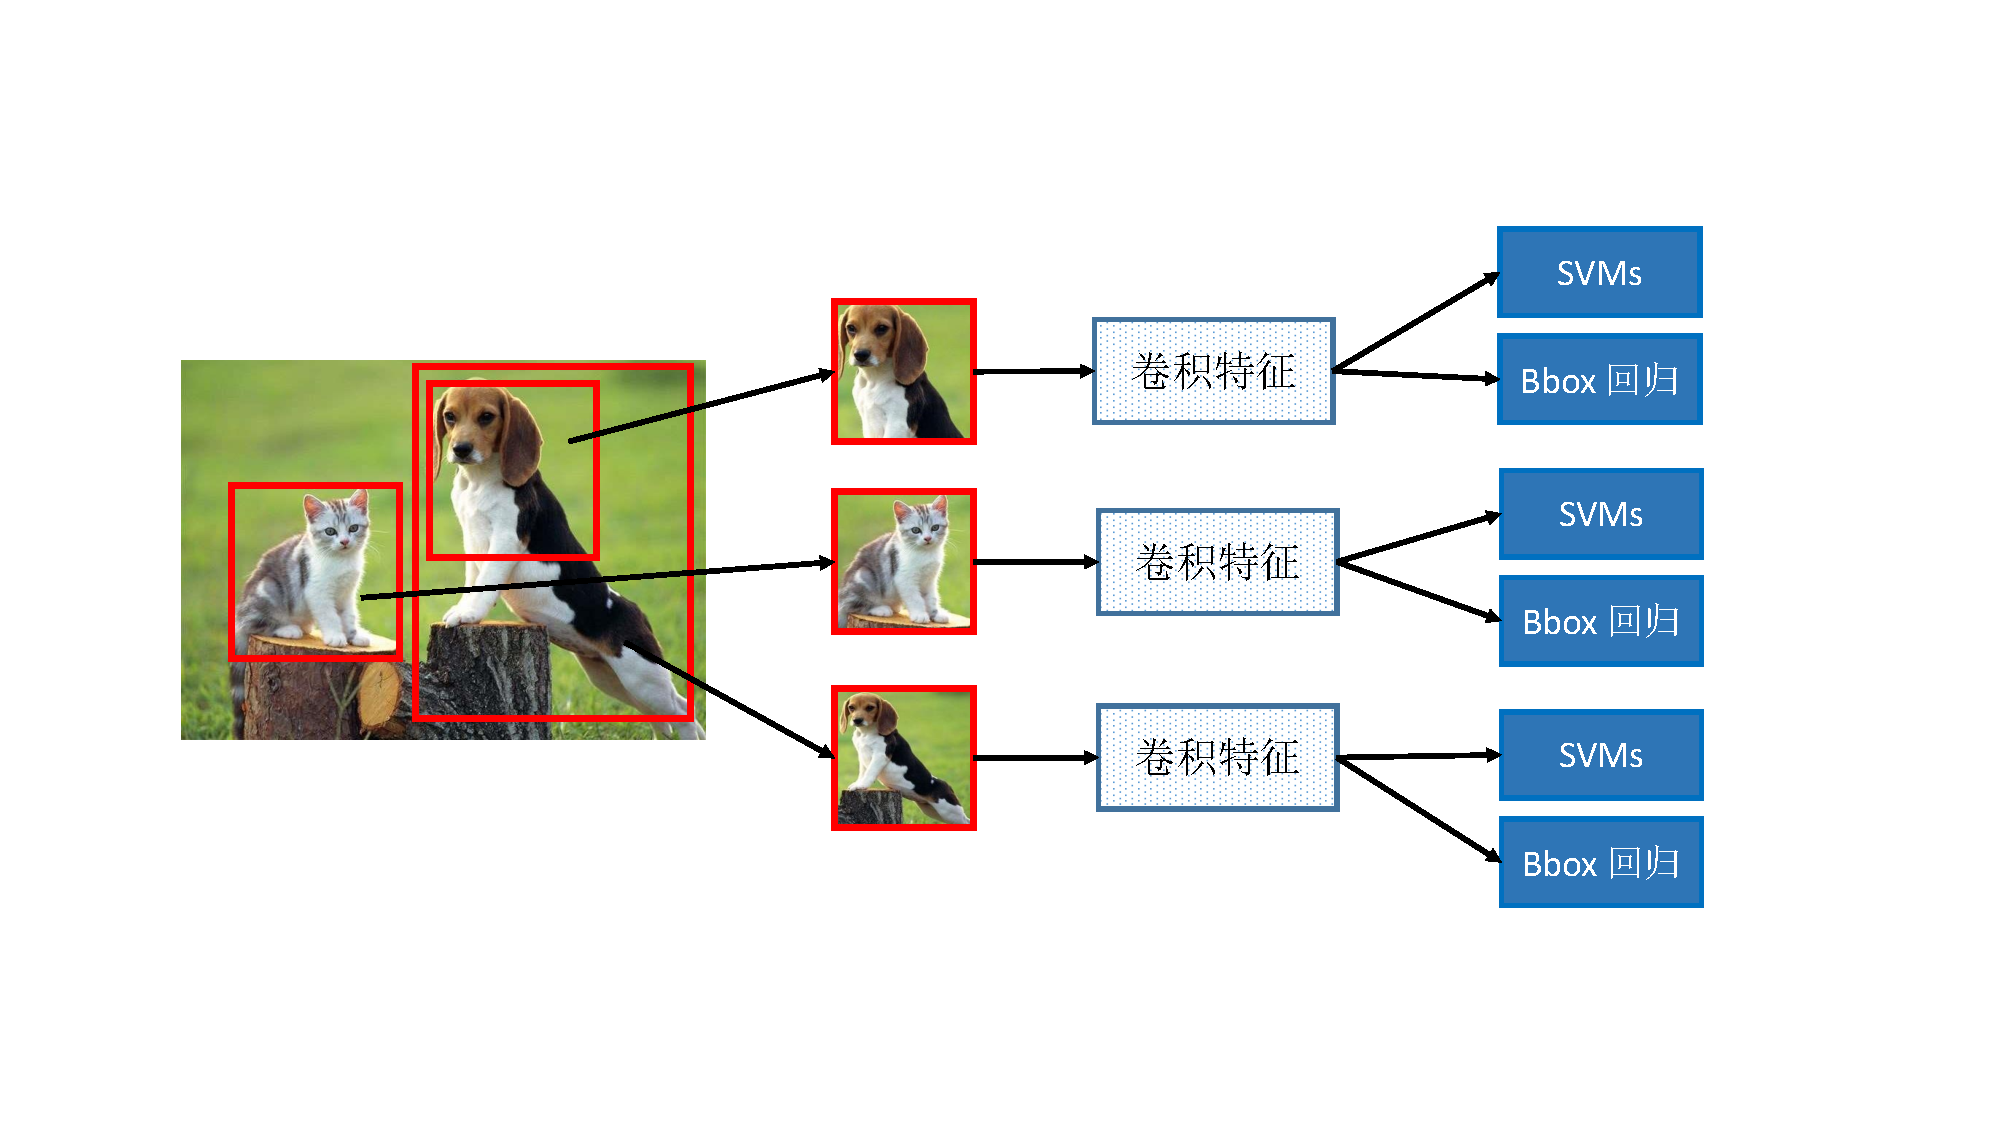
\includegraphics[trim={3cm, 3.5cm, 5cm, 4cm}, clip, width=\textwidth]{./imgs/RCNN.pdf}
	\caption{R-CNN 结构示意图,红框为由选择性搜索算法生成的候选框。}
	\label{fig:rcnn}
\end{figure}

\begin{figure}[!t]
	\centering
	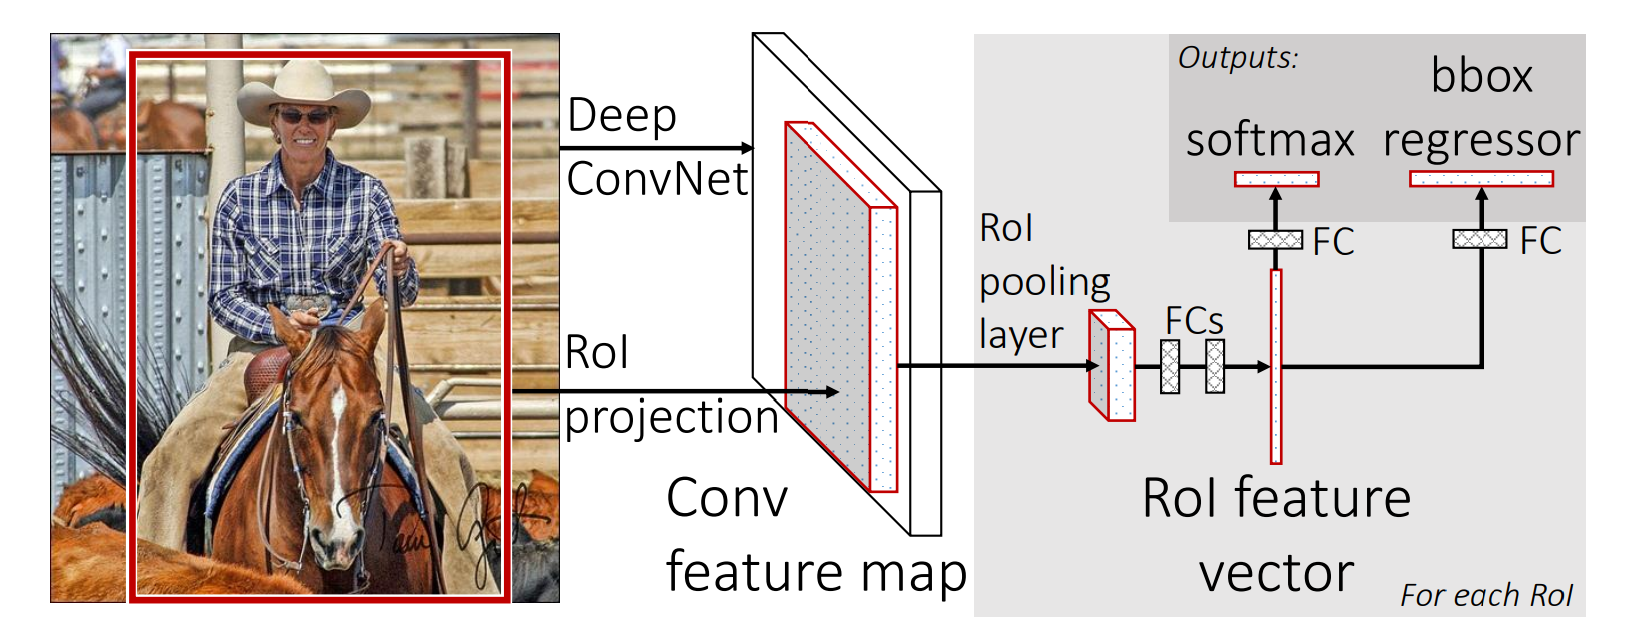
\includegraphics[width=0.95\textwidth]{./imgs/fast-rcnn.png}
	\caption{Fast-RCNN 结构示意}
	\label{fig:fast-rcnn}
\end{figure}


R-CNN可以说是利用深度学习技术进行目标检测的开山之作,其基本结构如图\ref{fig:rcnn}所示。 该工作使用选择性搜索(Selective Search)算法\cite{UijlingsSelective}代替传统的滑动窗口来提取候选区域, 并且利用神经网络对图片进行特征提取,然后利用提取的卷积特征回归更加精确的边界框,同时使用SVMs进行类别判断。该工作奠定了两阶段目标检测框架的基本结构,即一个区域提取(Region Proposal)算法用于提取输入图像中可能是目标的区域, 一个CNN网络用于提取区域特征,一个分类算法用于类别鉴定以及一个回归模型用于回归出精确的物体边界框。2015年,在R-CNN的基础上,RBG(Ross B. Girshick) 又提出了Fast-RCNN算法。该算法借鉴了SPP-Net\cite{7005506}的实现,对R-CNN做了改进,使得检测性能进一步提高,其结构如 \figurename \, \ref{fig:fast-rcnn}所示。具体而言有两个重大改进:(1)将候选区域提取阶段移到了图像特征提取之后,即只对原图做一次卷积,然后在特征图上运行候选区域提取算法得到候选区域特征图,然后将每一个提取的特征块输入RoI(Region of interest)层(结构如图\ref{fig:roi}所示)来将不同尺度的特征图转化为相同维度的密集特征向量,之后送入全连接层进行后续处理;(2)R-CNN训练神经网络提取图像特征,之后用支持向量机进行分类以及用一个回归模型精修边界框。而Fast-RCNN则利用两个全连接层(一个分类分支与一个回归分支) 将分类与回归任务整合到一个模型里联合训练,这为之后的目标检测端对端训练打下了基础。

\begin{figure}[t]
	\centering
	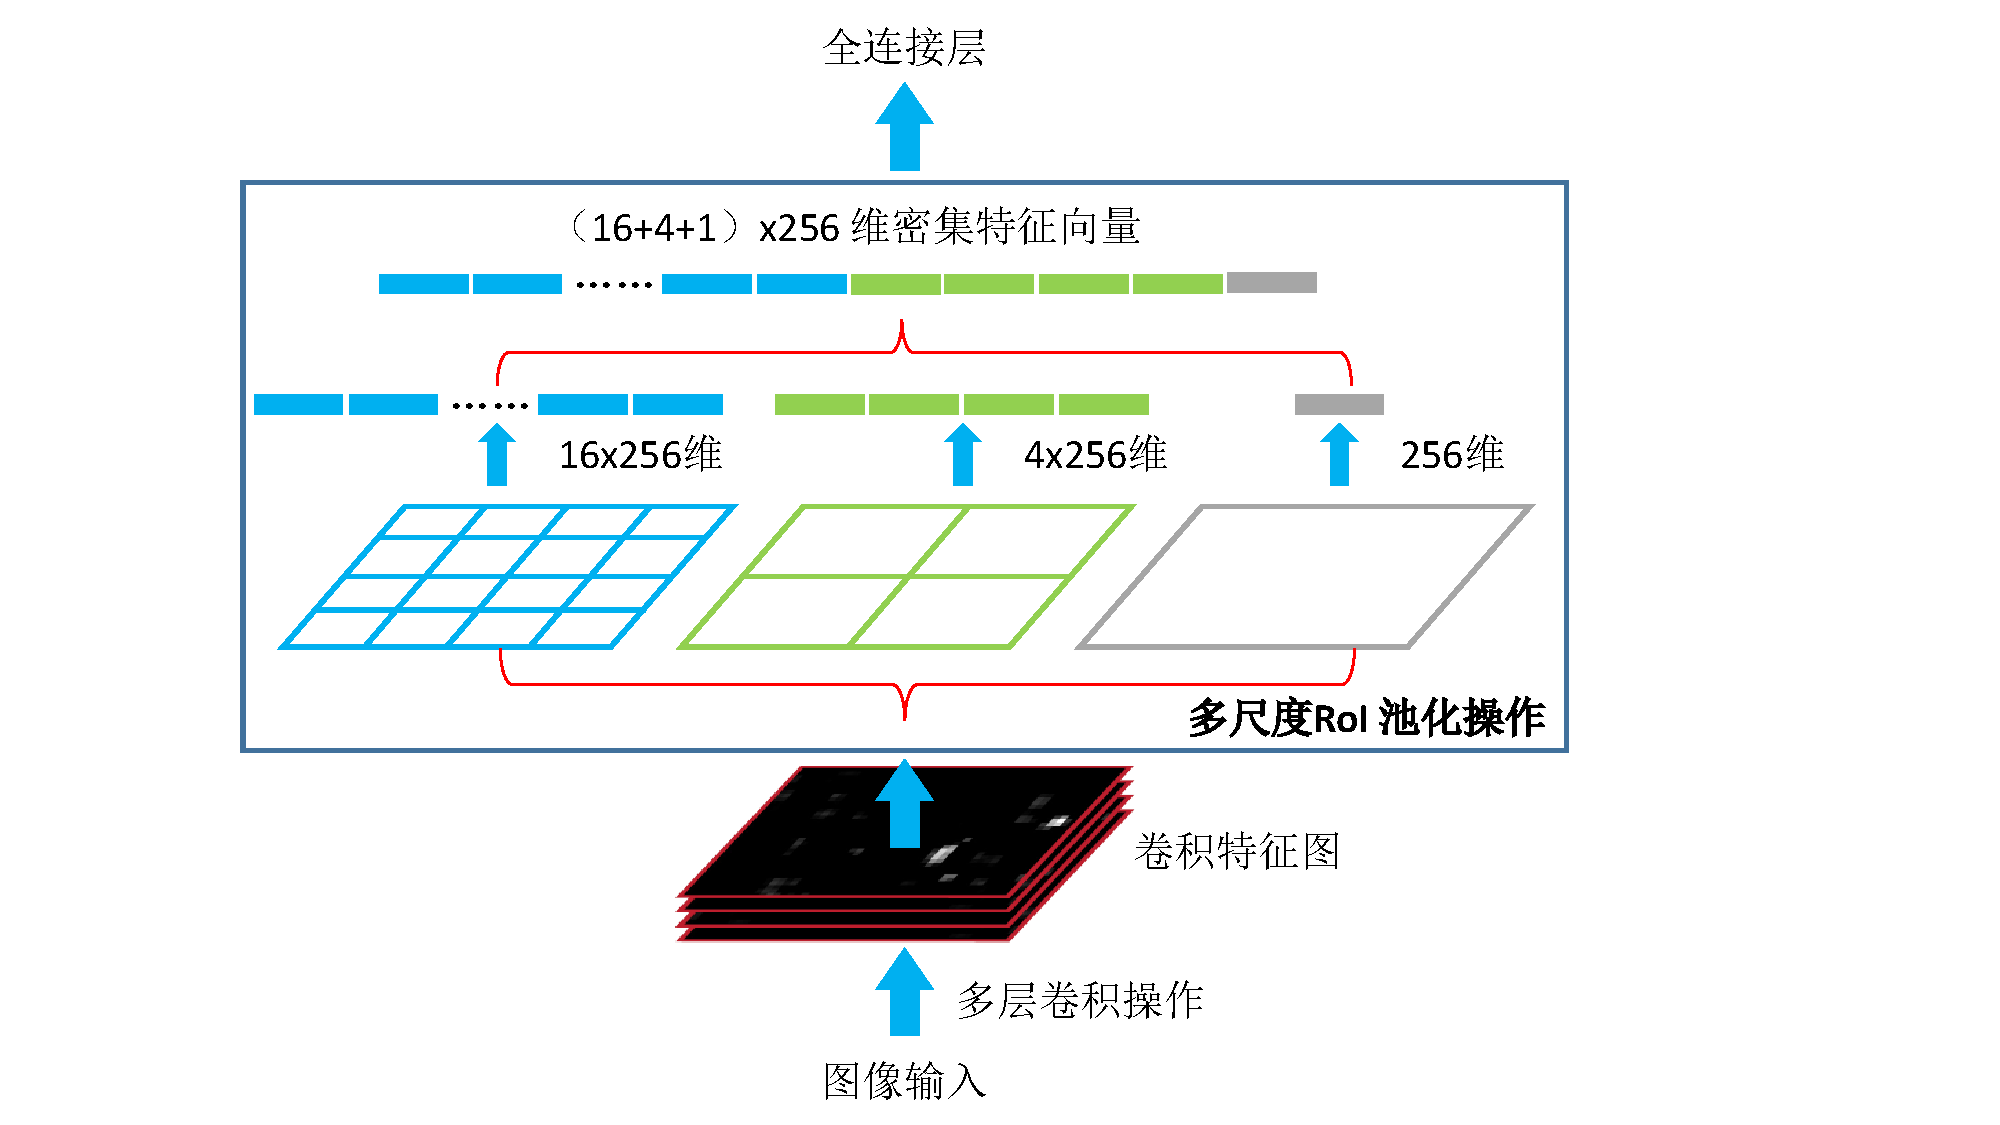
\includegraphics[trim={4cm, 0cm, 7cm, 0cm}, clip,width=0.8\textwidth]{./imgs/roi.pdf}
	\caption{RoI层将不同尺寸的特征图转换为密集特征向量,然后输入全连接层。图中为多尺度RoI池化操作,Fast-RCNN原工作使用的是单尺度,譬如只有4x4的池化操作。}
	\label{fig:roi}
\end{figure}


尽管Fast-RCNN 相对于 R-CNN 已经提速了不少,但要实现实时检测,网络运行速度还是不够,其中主要的瓶颈是候选区域提取阶段十分耗时。基于CPU实现的 Selective Search 算法提取一幅图像的所有候选区域(Proposals)需要约2s时间,效率更高的 EdgeBoxes\cite{Zitnick2014Edge} 算法虽然在一定程度上提高了候选区域提取的准确率和速度,但处理一幅图像仍然需要0.2s。为了解决这个问题,2015年微软亚洲研究院提出了Faster-RCNN算法,该算法引入了候选区域提取网络(Region Proposal Network,RPN),使用神经网络取代传统的区域提取算法,将单幅图像候选区域提取时间缩短到了10ms。下一小节将以Faster-RCNN为代表,重点介绍两阶段物体检测框架的结构以及实现细节。

\subsubsection{Faster-RCNN框架结构}

\begin{figure}[!t]
	\centering
	\begin{minipage}[t]{0.4\textwidth}
		\centering
		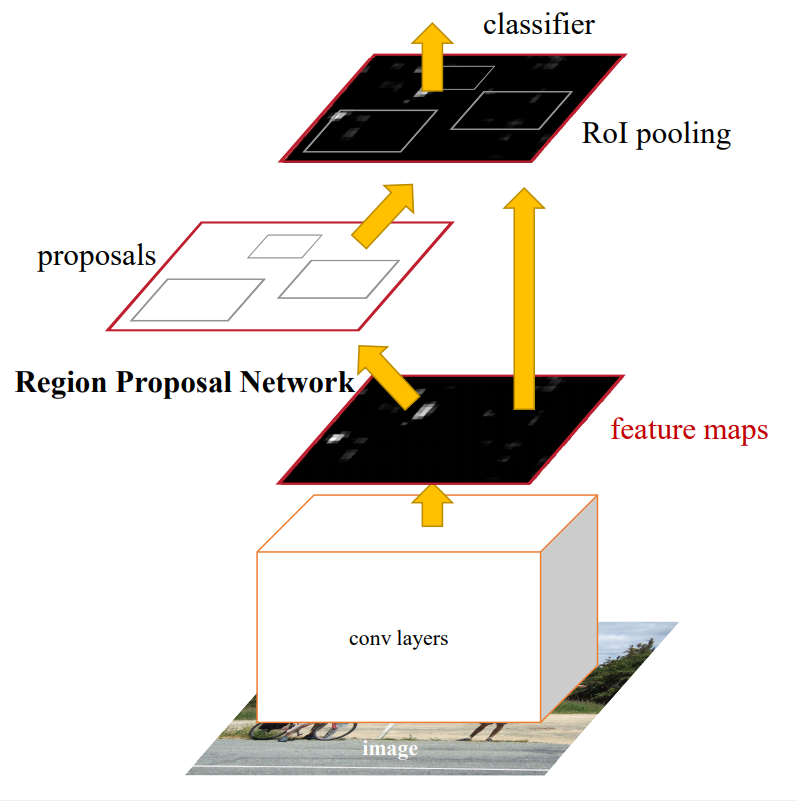
\includegraphics[width=\textwidth]{./imgs/faster-rcnn.png}
		\caption{Faster-RCNN 结构示意}
		\label{fig:faster-rcnn}
	\end{minipage}
	\begin{minipage}[t]{0.58\textwidth}
		\centering
		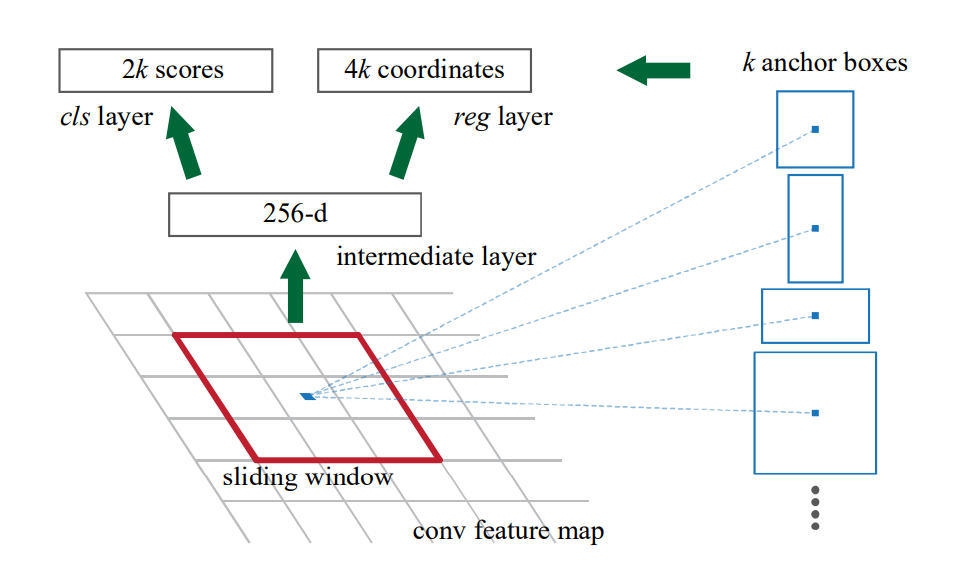
\includegraphics[width=\textwidth]{./imgs/rpn.png}
		\caption{RPN 结构示意}
		\label{fig:rpn}
	\end{minipage}
\end{figure}


Faster-RCNN框架由两大模块组成,候选区域提取模块(RPN)和检测模块, 如 \figurename \, \ref{fig:faster-rcnn} 所示。其中RPN取代了原来的区域提取算法,而检测模块和Fast-RCNN类似,都是由卷积层以及全连接层组成。对于Faster-RCNN网络,首先输入一幅图像,图像经过卷积神经网络提取特征得到卷积特征图(feature maps),然后特征图输入到RPN模块预测得到候选框(proposals),之后根据候选框去特征图中截取相应的特征块。这时的特征块由于尺寸不一样(为了满足物体的尺度多样性,候选框的尺寸不一样),不能直接输入到检测模块进行分类和回归,而是要通过RoI池化操作得到相同尺寸的密集特征向量,然后送入分类分支和回归分支分别预测得到分类结果以及预测框的位置信息。RPN是Faster-RCNN新引进的模块,其原理如\figurename \, \ref{fig:rpn}所示。在特征提取网络生成的特征图($M \times N$)上,使用$k$ 个 $n \times n$ 的卷积核卷积生成$M \times N \times k$个维度为256的中间特征向量,之后输入候选框分类分支和回归分支,分别用来预测候选框的类别(前景/背景,$M \times N \times 2 \times k$)以及候选框的位置信息(中心点坐标$x, y$以及宽高$w, h$, 整体维度为$M \times N \times 4 \times k$)。其中,$k$ 也可以表示为对于特征图上的每一个像素点(或者称为锚点),都负责预测$k$个锚点框(anchor boxes)。另外,为满足候选框的尺寸变化,这$k$个锚点框会设置不同的尺寸和长宽比。原始的Faster-RCNN中设置了三种不同的尺寸:$128\times 128$,$256 \times 256$, $512 \times 512$(px), 也设置了三种不同的长宽比:$1:1$, $1:2$, $2:1$。因此 $k = 3 \times 3 = 9$,意味着每个锚点负责预测9个不同的候选框。

\subsubsection{Faster-RCNN网络训练}
构建好了网络结构,网络的训练还需要准备训练数据,明确损失函数等。目标检测的训练数据一般有公开的数据集,如COCO\footnote[5]{http://cocodataset.org/},PASCAL\footnote[6]{http://host.robots.ox.ac.uk/pascal/VOC/}等,然而Faster-RCNN还需额外训练RPN网络,因此需要额外准备RPN网络训练的标签数据。候选框标签的生成需要借助真实标签数据:首先根据上文提到的锚点的概念,以特征图尺寸为参照生成$M \times N \times k$个候选框(一共有$M \times N$个锚点,每个锚点有$k$个不同尺寸的锚点框),然后根据候选框与真实物体框的重叠程度(一般以候选框与真实框的交并比IoU为量化指标)计算每个候选框的得分。候选框的得分可作为其划分前景类还是背景类的依据,譬如得分大于0.65划分为前景,小于0.35划分为背景,而得分在[0.35,0.65]之间的候选框则忽略不计,这样就得到了训练RPN网络的标签数据。

\begin{figure}[t]
	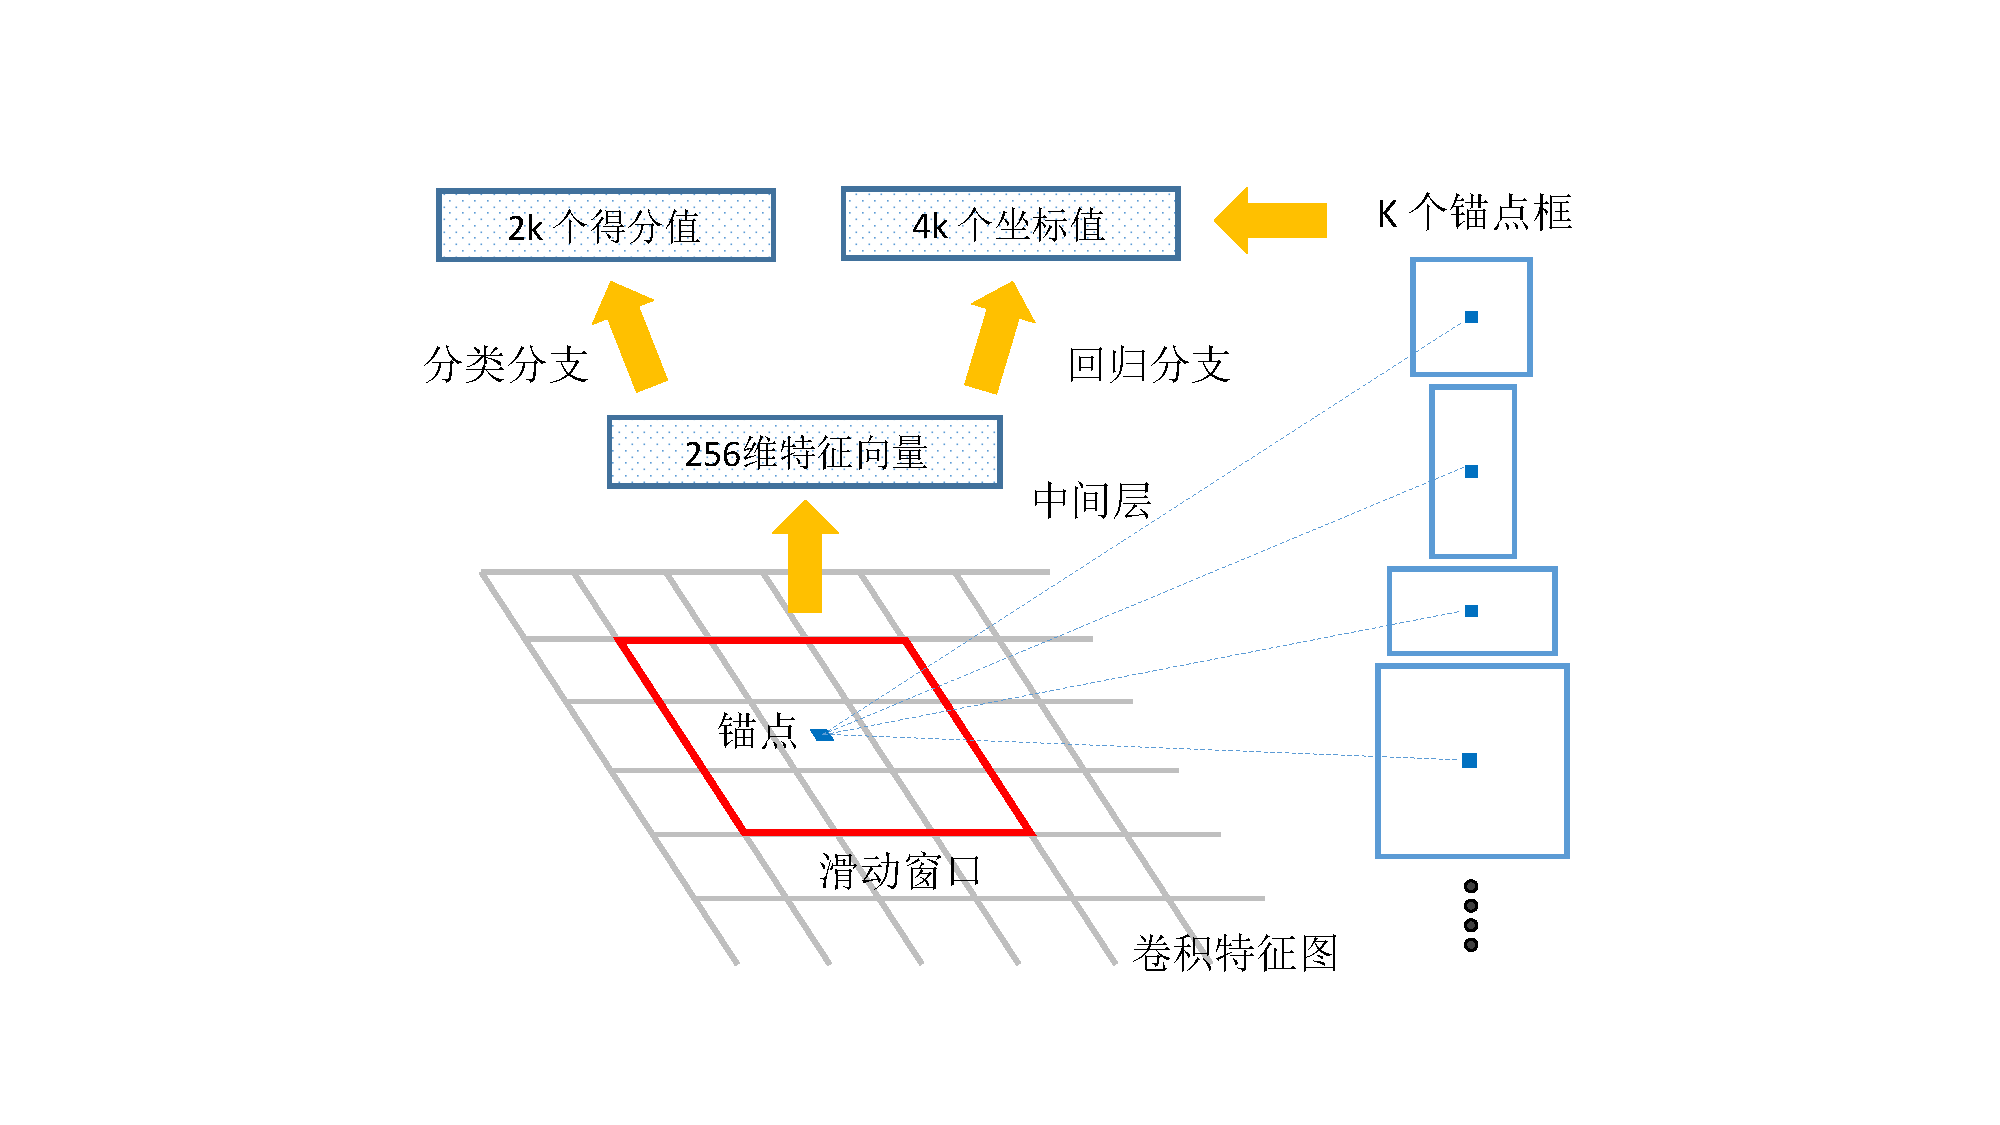
\includegraphics[trim={5cm, 2cm, 5cm, 3cm}, clip,width=0.9\textwidth]{./imgs/rpn.pdf}
	\caption{候选框提取网络结构细节。}
	\label{fig:rpn}
\end{figure}


Faster-RCNN的损失函数由两部分构成,RPN损失和Fast-RCNN损失,并且这两部分损失又都包括两类损失,分类损失和回归损失。
\begin{equation}
L(\{p_i\},\{t_i\}) =\frac{1}{N_{cls}} \sum_{i}L_{cls}(p_i, p^*_i) + \lambda \frac{1}{N_{reg}} \sum_{i} p^*_i L_{reg}(t_i,t^*_i)
\label{con:rpn_loss}
\end{equation}
RPN损失函数如公式 \ref{con:rpn_loss} 所示,其中第一部分为分类损失,第二部分为回归损失。分类损失计算了RPN预测生成的候选框类别的交叉熵损失$L_{cls}$, 其公式如 \ref{con:cross_entropy}所示。其中$p_i$为预测生成的候选框类别,$p^*_i$是标签值。RPN网络生成的候选框分为前景和背景,前景标签为1,背景为0,是一个二分类问题。
\begin{equation}
L_{cls} = -\log[p^*_ip_i + (1-p^*_i)(1-p_i)]
\label{con:cross_entropy}
\end{equation}
在训练中,RPN网络生成的$M \times N \times k$个候选框,然而并不是每个候选框都会纳入损失值的计算范围,因为这些候选框有很多会重叠在一起。Faster-RCNN使用了非极大值抑制(Non-Maximum Suppression,NMS)算法进行初步筛选,减少重叠的候选框。NMS算法详细流程如算法 \ref{alg:nms} 所示:对于RPN生成的候选框集合 $\mathcal{B}$以及对应的置信度集合$\mathcal{S}$,首先选择对应最大置信度的候选框$M$,将其从$\mathcal{B}$中移除并加入最终候选框集合$\mathcal{D}$;然后遍历$\mathcal{B}$,移除与$M$的交并比(Intersection of union, IoU)大于阈值$\epsilon$的框;重复此过程,直到$\mathcal{B}$为空。通过选择合适的阈值(Faster-RCNN中为0.7),NMS算法可以过滤掉大部分重叠的候选框,之后从中随机选取$N_{cls}$个候选框计算分类损失,在Faster-RCNN中$N_{cls} = 256$。
\begin{algorithm}[t]
	\caption{非极大值抑制算法}
	\label{alg:nms}
	\textbf{输入: } $\mathcal{B}=\{b_1,...,b_N\}$,RPN生成候选框集合; $\mathcal{S}=\{s_1,...,s_N\}$, 生成候选框对应的置信度集合; $\epsilon$, 置信度阈值 \\
	\textbf{初始化:} $\mathcal{D} \leftarrow$ \{ \},最终候选框集合 \\
	\While{$\mathcal{B} \neq \emph{empty }$}{
		$m \leftarrow \emph{argmax } \mathcal{S}$ \\
		$\mathcal{M} = b_m$ \\
		$\mathcal{D} \leftarrow \mathcal{D} \bigcup \mathcal{M}; \, \mathcal{B}  \leftarrow\mathcal{B} - \mathcal{M}$ 
	 
		\For{$b_i \emph{ in } \mathcal{B}$}{
			\If{$\emph{IoU}(\mathcal{M},b_i) \leq \epsilon$}{
				$\mathcal{B} \leftarrow \mathcal{B} - b_i; \, \mathcal{S} \leftarrow \mathcal{S} - s_i$
			}
		}
	}
	\textbf{输出: } $\mathcal{D},\mathcal{S}$
\end{algorithm}

RPN回归损失计算预测候选框的$Smooth_{L1}$损失$L_{reg}$,注意到RPN回归损失只计算前景的损失,因此$L_{reg}$前需乘以$p^*_i$(前景为1,背景为0)。$N_{reg} = N_{cls}$,为经过NMS算法过滤后随机选择的候选框数。$Smooth_{L1}$损失公式如\ref{con:smooth_l1}所示,
\begin{equation}
L_{reg}(t_i,t^*_i) = 
\begin{cases}
0.5(t_i-t^*_i)^2 & |t_i-t^*_i| \leq 1 \\
|t_i-t^*_i| - 0.5 & \text{否则}
\end{cases}
\label{con:smooth_l1}
\end{equation}
其中 $t_i$和$t^*_i$分别对应预测候选框以及真实候选框的信息。其中$t_i = (t^x_i, t^y_i,t^w_i,t^h_i)$ 为一四维偏移向量,其计算公式如\ref{con:offsets}所示。其中$(x_a,y_a,w_a,z_a)$分别是对应锚点框中心点坐标以及宽高。从损失值的计算可以看出,RPN并不直接回归出候选框的位置信息,而是回归候选框与对应的锚点框的偏移量,这种处理有利于稳定网络的训练过程,也有利于网络的收敛。
\begin{equation}
t_x = \frac{x - x_{a}}{w_{a}}; \, t_y = \frac{y - y_{a}}{h_{a}}; \,
t_w = \log(\frac{w}{w_{a}}); \, t_h = \log(\frac{h}{h_{a}})
\label{con:offsets}
\end{equation}

检测模块的Fast-RCNN的损失和RPN类似,同样由分类损失和回归损失组成。不过RPN的分类损失是二分类的交叉熵损失,而Fast-RCNN的分类损失是多分类的交叉熵损失,不过将类别标签转化为one-hot向量后并没有本质区别。和RPN类似,Fast-RCNN也不针对所有预测框计算损失,而是先通过更严格的NMS算法(Faster-RCNN中阈值设置为0.3)筛选出一批重叠度低、得分高的预测框,然后随机选择一定数量的预测框进行损失值计算。Fast-RCNN的回归损失基本也和RPN的一致,也不直接回归真实框的位置信息,而是回归物体真实框与锚点框的偏移量,偏移量的编码方式与上文RPN中的类似。

\subsection{单阶段目标检测}
\label{one-stage}
从 R-CNN 到 Fast-RCNN 再到 Faster-RCNN,两阶段目标检测方法一直采用先计算出候选区域然后再在候选区域上提取特征进行分类和回归的算法流程。该模式可以获得很好的检测精度,然而在检测速度上还不是很理想,最好的Faster-RCNN只能达到0.2s一帧的检测速度,离实时检测还有很大差距。单阶段目标检测方法则提供了另一种更为直接的设计思路:不显式计算候选框提取候选区域,而是通过神经网络直接预测物体的位置与类别。该模式的代表工作有YOLO\cite{redmon2016you}系列以及SSD\cite{liu2016ssd},本节以YOLO为例,介绍单阶段目标检测的典型框架结构以及实现原理。


\begin{figure}[!t]
	\centering
	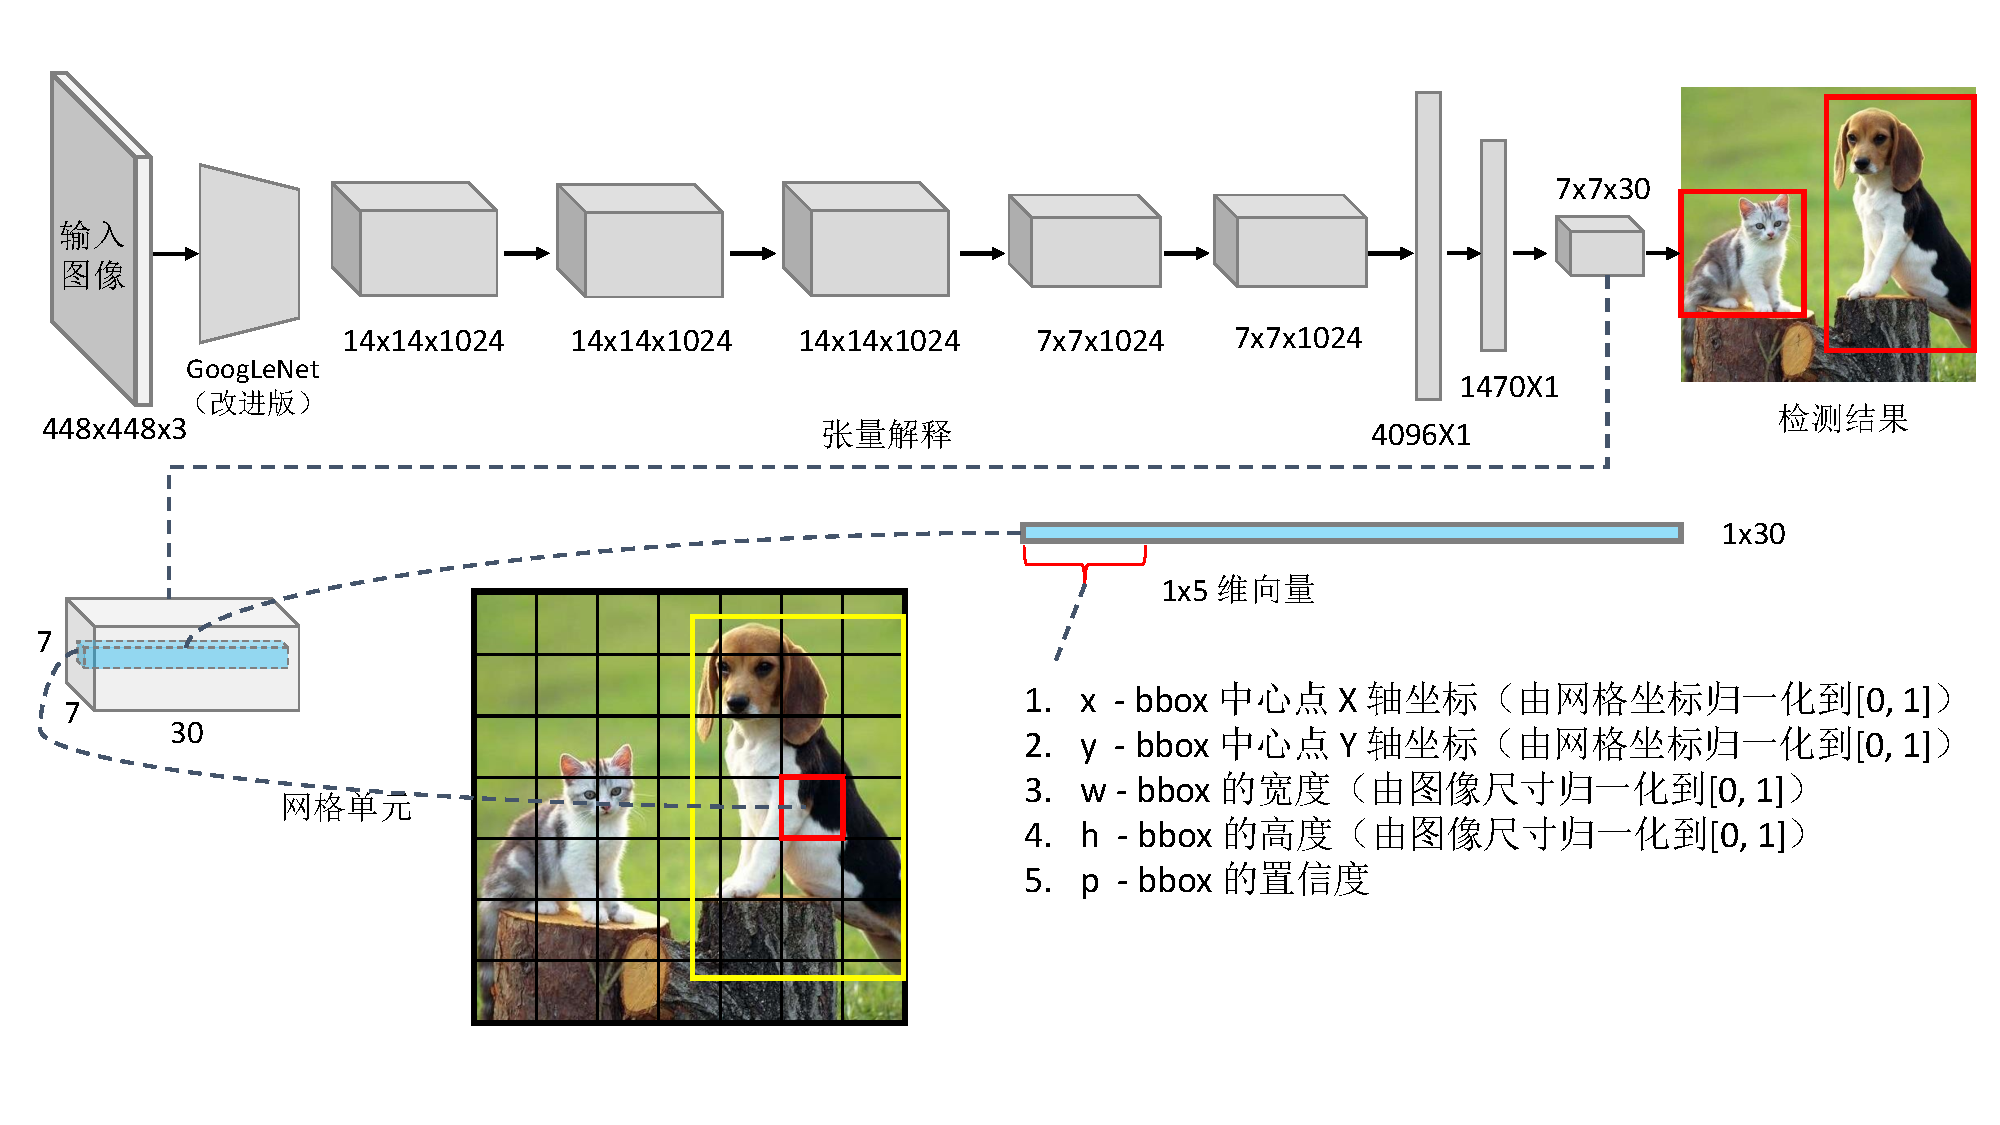
\includegraphics[trim={0.5cm, 2cm, 0cm, 1cm}, clip,width=\textwidth]{./imgs/yolo.pdf}
	\caption{YOLO结构示意图。}
	\label{fig:yolo}
\end{figure}


YOLO的整体架构如\figurename \, \ref{fig:yolo}所示。与R-CNN系列工作不同,YOLO将目标检测任务整体作为一个回归任务来解决。输入一张图像,YOLO首先将输入图像宽高调整到$448 \times 448$,然后输入到由GoogLeNet\cite{7298594,7780677}改进的特征提取卷积网络中,最后输出一个维度为$S \times S \times (B \times 5 + C)$的张量$\mathcal{T}$(YOLO中张量维度为$7 \times 7 \times 30$)。$\mathcal{T}$可以这么理解,首先将一幅图像分成$S \times S$ (YOLO是$7\times 7$)个网格,对于每个网格单元$s$,其对应着$\mathcal{T}$中的一项维度为$1 \times (B \times 5 + C)$的向量$t$。如果一个目标物体的中心落在$s$上,则$s$负责预测该物体,预测结果编码在向量$t$中。$t$维度为$B \times 5 + C$,其中 $B$ 表示每个网格预测$B$个尺度变化的边界框(YOLO中$B=2$);$5$编码了bbox的信息,分别是$(x,y,w,h,c)$,代表bbox中心点坐标、宽高以及置信度;$C$ 表示需要预测$C$个类(YOLO中$C=20$),每个值表示预测为该类的概率值$Pr(class_i|object)$。

和Faster-RCNN类似,YOLO也不是直接回归出物体边界框的实际坐标和宽高,而是bbox相对于单元格的偏移量。对于向量$t=(x,y,w,h,c)$,$(x,y)$的计算公式如\ref{con:yolo_xy}所示,其中$(x_c,y_c)$是bbox中心点的实际坐标,$(w_i, h_i)$是图像的宽高,$x_{col}, y_{col}$是单元格的坐标。最终预测出来的$(x,y)$是经过归一化处理的、中心相对于单元格的偏移。$(w,h)$的计算公式如\ref{con:yolo_wh}所示,是bbox相对于整张图像的比例。置信度$c$的计算公式如\ref{con:yolo_c}所示,由两部分组成,$Pr(object)$表示单元格内是否有物体,有为1,没有则为0;$IoU^{Truth}_{Pred}$表示bbox位置的准确度,用IoU衡量。
\begin{gather}
x = \frac{x_c}{w_i}S - x_{col}; \, y = \frac{y_c}{h_i}S - y_{row} 
\label{con:yolo_xy}\\
w = \frac{w_b}{w_i}; \, h = \frac{h_b}{h_i}
\label{con:yolo_wh}\\
c = Pr(object)*IoU^{Truth}_{Pred}
\label{con:yolo_c}
\end{gather}

在测试阶段,网络最终输出也为一个$S \times S \times (B \times 5 + C)$的张量,其中包含$S \times S \times B$个预测框,每个预测框的最终概率为 $Pr(class_i|object)* c$,综合了定位误差和分类误差。最后这$S \times S \times B $ 列的结果会送入NMS算法去除重复的检测框,得到最终的检测结果。

YOLO的损失函数设计比较复杂,如公式\ref{con:yolo_loss}所示。YOLO的损失函数都采用平方和损失,可分为五部分来看:
\begin{equation}
\begin{split}
L_{yolo} &= \lambda_{coord} \sum^{S^2}_{i=0} \sum^{B}_{j=0} \mathds{1}^{obj}_{i,j} (x_i - \hat{x}_i)^2 + (y_i - \hat{y}_i)^2 \\
&+ \lambda_{coord} \sum^{S^2}_{i=0} \sum^{B}_{j=0} \mathds{1}^{obj}_{i,j} \left(\sqrt{w_i} - \sqrt{\hat{w}_i}\right)^2 + \left(\sqrt{h_i} - \sqrt{\hat{h}_i}\right)^2 \\
&+ \sum^{S^2}_{i=0} \sum^{B}_{j=0} \mathds{1}^{obj}_{i,j}\left(C_i -\hat{C}_i\right)^2\\
&+ \lambda_{noobj} \sum^{S^2}_{i=0} \sum^{B}_{j=0} \mathds{1}^{noobj}_{i,j}\left(C_i -\hat{C}_i\right)^2\\
&+ \sum^{S^2}_{i=0}\mathds{1}^{obj}_{i}\sum_{c \in classes} \left(p_i(c) - \hat{p}_i(c)\right)^2
\end{split}
\label{con:yolo_loss}
\end{equation}
第一部分为bbox中心坐标的误差,其中$\mathds{1}^{obj}_{i,j}$表示判断第$i$个网格中第$j$个bbox是否负责预测该物体。第二部分为bbox宽高的误差,由于在对不同大小的bbox的预测中,小bbox预测偏离的容忍程度比大bbox要小很多,而平方和损失对bbox的尺度并不敏感。为了解决这个问题,YOLO使用宽高的平方根代替原来的宽高。第三部分为含有物体的bbox的置信度预测误差,第四部分为不含物体的bbox的置信度预测误差。最后一部分是对bbox类别预测的误差,其中$\mathds{1}^{obj}_{i}$表示是否有物体落在单元格$i$中。另外,为了平衡各种损失之间的比例,YOLO还加入了$\lambda_{coord}, \lambda_{noobj}$作为超参数平衡各部分损失。

YOLO由于没有显式的预测候选框的过程,因此检测速度很快。但是由于其中网格的划分不可能十分细致,因此YOLO对相互靠的很近的物体(中心可能落在同一个单元格内)、以及小物体检测效果不好。这是由于一个单元格只预测一个类,当物体重叠时,会出现几个不同物体的中心都落在一个单元格的情况。另外,YOLO对于同一类物体出现不常见的长宽比等情况的泛化能力较差,这些问题在其YOLO的后续工作YOLOv2\cite{8100173}、YOLOv3\cite{RedmonYOLOv3}中有探究。

\subsection{三维目标检测}
\label{3d_detection}

\begin{figure}[!t]
	\centering
	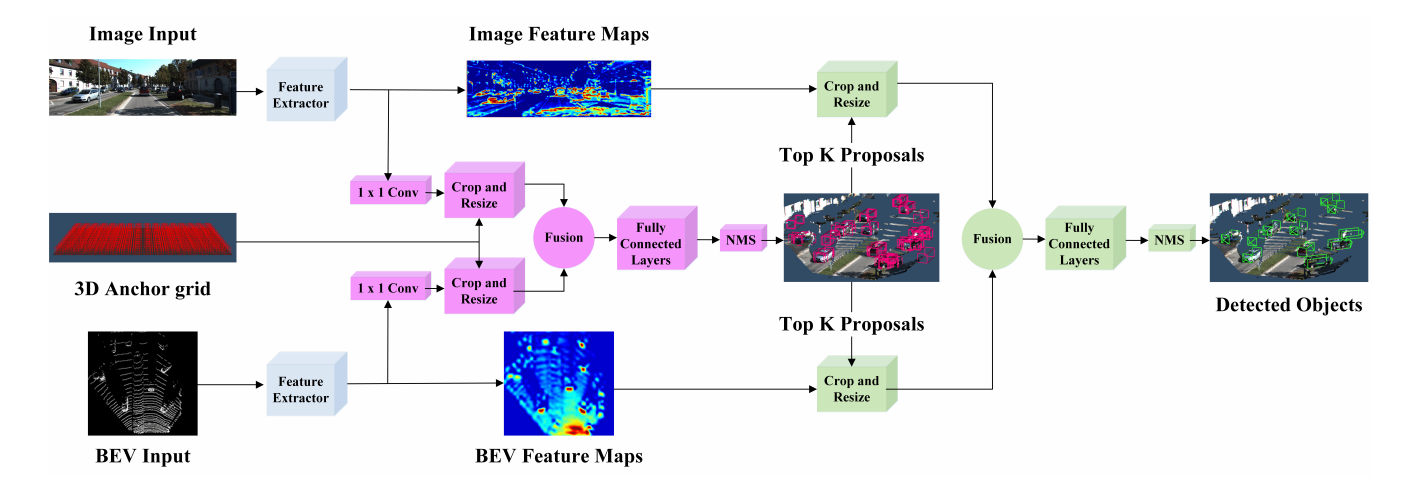
\includegraphics[width=\textwidth]{./imgs/avod.png}
	\caption{AVOD 结构示意图\cite{ku2018joint}。}
	\label{fig:avod}
\end{figure}


三维目标检测任务需要明确目标在三维环境中的位姿状态,包括目标在三维世界的坐标,形状以及朝向。然而,将基于图像的二维目标检测推广到三维对于模型框架本身来说并没有多大变化。以两阶段二维目标检测为例,将其推广到三维空间时,输入数据需要从二维转化到三维,相应的特征提取模块、候选区域提取网络以及结果输出也需要做出调整。两阶段三维目标检测比较有代表性的如AVOD\cite{ku2018joint},网络结构如图\ref{fig:avod}所示。对于特征提取模块,由于AVOD使用的是基于投影的方法编码点云特征,将深度维度转化为通道,和二维RGB图像的特征提取类似,因此不需要做出很大的改变。但是对于其他点云编码方式,可能需要将二维卷积换成三维卷积以完成对三维数据的特征提取。对于RPN模块,AVOD使用的是3D锚点框,提取候选区域特征时是将3D候选框投影到图像以及点云BEV平面,这一点和二维目标检测有很大不同。对于最终的预测框结果输出,AVOD需要输出三维环境下的目标位姿信息,和二维目标检测只需要输出目标中心点坐标以及宽高不同。而在网络训练阶段,损失值的设置也需要将二维框回归的损失转化为三维框回归损失,而对于需要预测目标三维朝向的,还需要加入朝向预测的损失。不过这些损失值的设置基本和二维目标检测类似,这里不做过多介绍。对于单阶段三维物体检测,也需要根据维度的变化对网络结构做出相应的调整,不过整体来说也和二维单阶段目标检测类似。

%对于单阶段三维目标检测,由于不涉及显式的候选框提取网络,因此只需要在数据输入、网格划分以及输出结果设置上调整成三维模式即可。典型的代表有VoxelNet\cite{zhou2018voxelnet},网络结构如图\ref{fig:voxelnet}所示。VoxelNet直接输入三维点云原始数据,并在三维空间中划分网格(体素),让每个非空体素负责预测中心点落入其中的目标。VoxelNet 借鉴了PointNet\cite{qi2017pointnet}中点云特征提取方法,将点云特征编码成了稀疏的四维张量,并通过三维卷积进一步提取特征,最后传入多尺度的候选区域提取模块进一步
%
%\begin{figure}[!t]
	\centering
	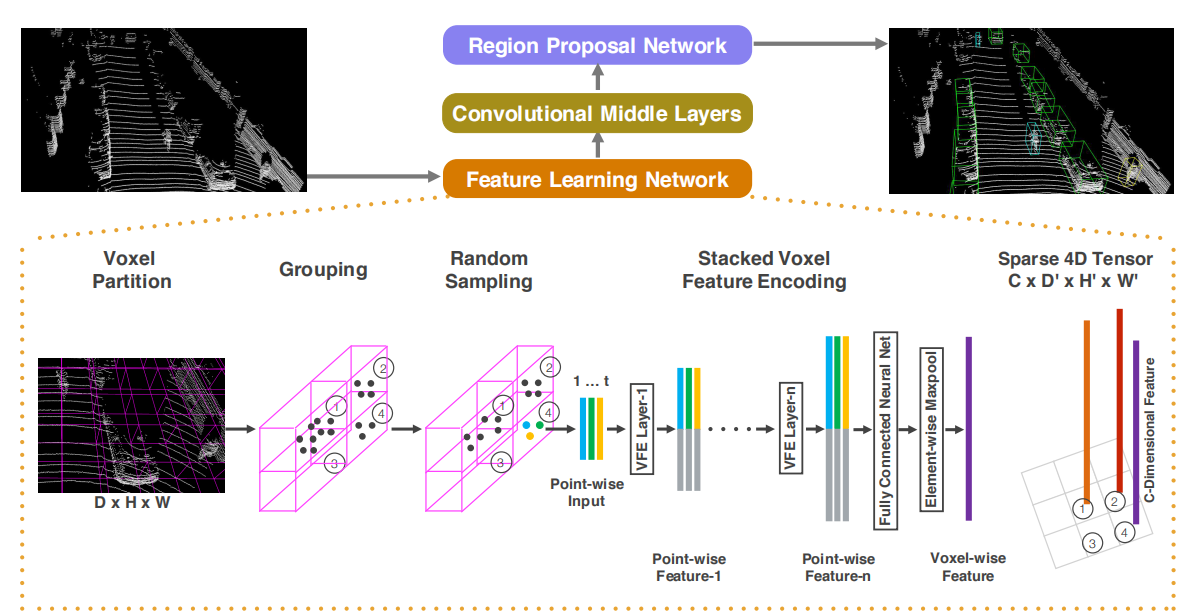
\includegraphics[width=\textwidth]{./imgs/voxelnet.png}
	\caption{VoxelNet 结构示意图\cite{zhou2018voxelnet}。}
	\label{fig:voxelnet}
\end{figure}


\section{目标跟踪}
\label{object_tracking}
由于本工作也涉及到一些目标跟踪方面的应用,因此本章将简单介绍下目标跟踪的一些基本理论。目标跟踪问题是指给定第一帧物体的位置,根据算法预测出后续帧中该物体的位置。根据同时追踪物体的数量的不同,目标追踪分为单目标追踪(Single Object Tracking, SOT)和多目标追踪(Multiple Object Tracking, MOT)。SOT与MOT虽然都属于目标跟踪,但确是两个差别很大的研究方向。由于本工作只涉及到多目标跟踪,因此会重点介绍MOT,而单目标跟踪只会简单叙述其基本原理。

\subsection{单目标跟踪}
\label{single_tracking}

单目标跟踪算法有生成式方法与判别式方法两大类。前者首先使用外观模型提取目标的视觉特征,然后通过最小化候选目标与跟踪目标之间的距离或是误差来确定目标。这类方法侧重目标本身的特征提取,但是忽略了目标与背景的差异,在目标外观发生剧烈变化时容易出现目标漂移或丢失的情况。判别式方法则将目标跟踪看成二元分类问题,通过训练分类模型来将目标区域与背景区分。这类方法可以显著区分背景和目标,因此鲁棒性强,是近几年目标跟踪领域的主流方法\cite{Wang2015Understanding}。

\begin{figure}[t]
	\centering
	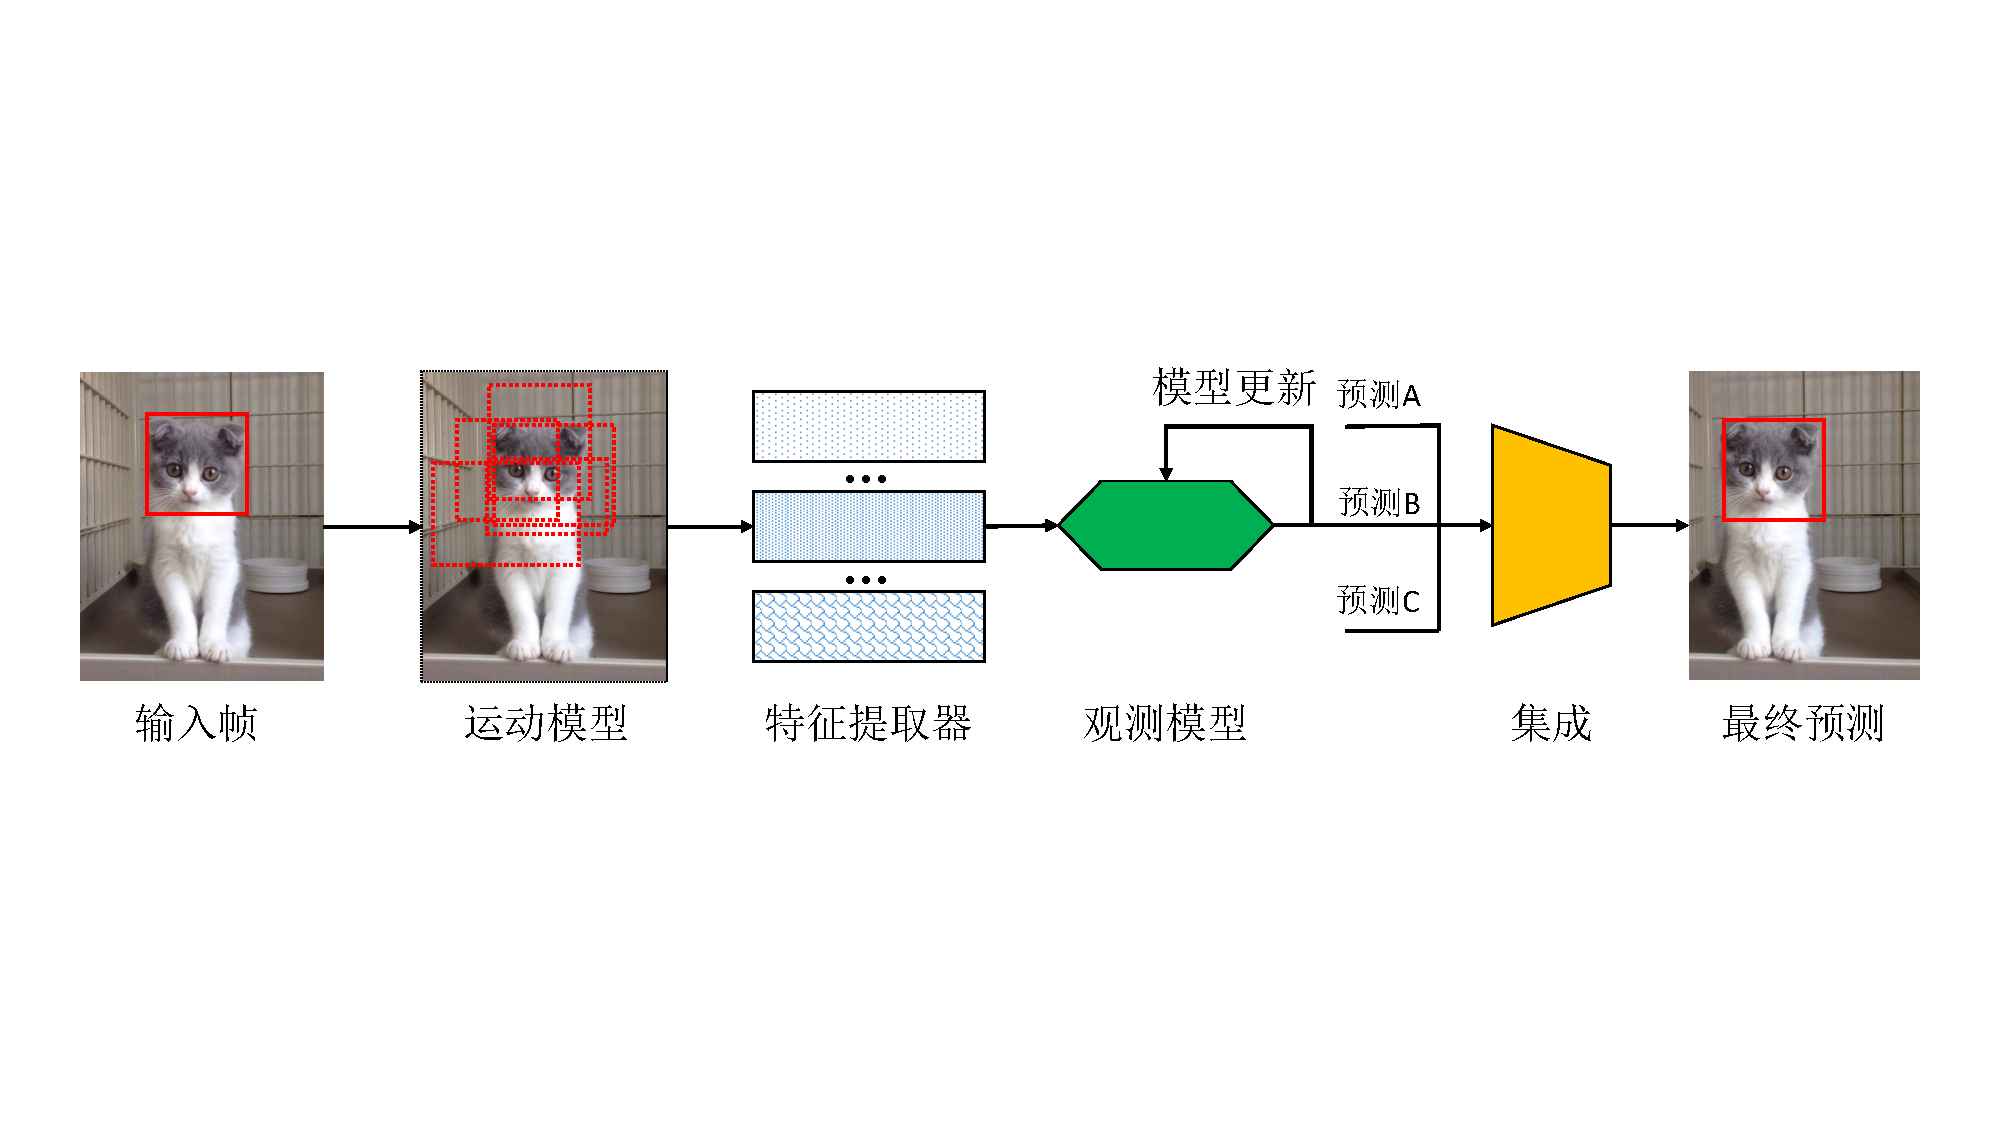
\includegraphics[trim={1cm, 6cm, 1cm, 6cm}, clip,width=\textwidth]{./imgs/sot_pipeline.pdf}
	\caption{单目标追踪流程图。整个流程由四个主要模块组成,分别是运动模块、特征提取模块、观测模块以及模型更新模块。}
	\label{fig:sot_pipeline}
\end{figure}


单目标跟踪算法的基本流程如图\ref{fig:sot_pipeline}所示。输入初始帧并初始化目标框,然后使用\textbf{运动模型}在下一帧中产生众多候选框,之后使用\textbf{特征提取器}提取这些候选框的特征,然后利用\textbf{观测模型}计算这些候选框的置信分数,然后找到最高评分对应的候选框作为预测的目标,或者通过集成方法融合多个候选框以得到更加精确的预测目标。最后,还需要通过\textbf{模型更新器}去更新观测模型。在整个流程中,共涉及到四个主要模块。其中,\textbf{运动模型}的目的是生成众多有效的候选框,其运行速度和质量直接决定了跟踪算法的性能。目前常用的运动模型有粒子滤波以及滑动窗口法。\textbf{特征提取器}决定跟踪系统使用何种特征表征目标,也是目标跟踪的关键。目前常用的特征有手工设计的特征以及使用网络学习的深度特征。其中,手工设计的特征有颜色特征、灰度特征、方向梯度直方图特征以及尺度不变特征等。\textbf{观测模型}可分为生成式模型和判别式模型,主要是评价候选框与目标的相似度,目前大多数跟踪方法主要集中在这一块设计。\textbf{模型更新器}的任务是根据当前跟踪目标更新观测模型,使其能够适应目标随时间的外观变化,这有利于防止跟踪过程中目标漂移或丢失情况的发生。

学术界针对单目标追踪有大量的研究,如首次将相关滤波引入单目标跟踪的MOSSE\cite{bolme2010visual}以及后续在此基础上发展的KCF\cite{henriques2014high}、DSST\cite{danelljan2014accurate}、C-COT\cite{danelljan2016beyond}以及ECO\cite{danelljan2017eco}等。另外,这些年基于孪生网络的单目标追踪模型发展迅速,如首先开创端对端深度学习式相关滤波方法先河的SiamFC\cite{bertinetto2016fully},以及加入了RPN应对尺度变化的SiamRPN\cite{li2018high}以及其改进版本DaSiamRPN\cite{zhu2018distractor}等。从近几年的单目标跟踪研究可以看出,深度学习技术也在该领域也引发了技术革新。

\subsection{多目标跟踪}
\label{mot}
相比于单目标跟踪,多目标跟踪任务需要同时跟踪场景中多个不同的目标,这些目标可能有着不同的外观特征和不同的运动方式,并且不同目标之间还会发生相互交汇、遮挡等交互活动,这些问题交杂在一起使得多目标跟踪算法的设计十分复杂与困难。目前学术界针对多目标跟踪的主流实现思路是基于检测的跟踪(Detection-Based Tracking),该方法要求先由一个目标检测器将每一帧的目标都检测出来,然后再使用框匹配算法将不同帧的同一物体相关联。按照可使用时间帧数据的不同,多目标跟踪算法可分为在线跟踪(Online Tracking)以及离线跟踪(Offline Tracking)。在线跟踪要求算法只能根据当前帧以及之前帧的信息得出下一帧的跟踪结果,而离线跟踪允许算法利用所有帧的信息,获取全局最优解。相对于离线跟踪,在线跟踪更适合实际应用场景。此外,还有一种近似在线跟踪(Near Online Tracking)方法,该方法利用当前帧一定窗口范围内的帧的信息得出下一帧的跟踪结果,是一种折中方法,只会导致些许延迟。

\begin{figure}[t]
	\centering
	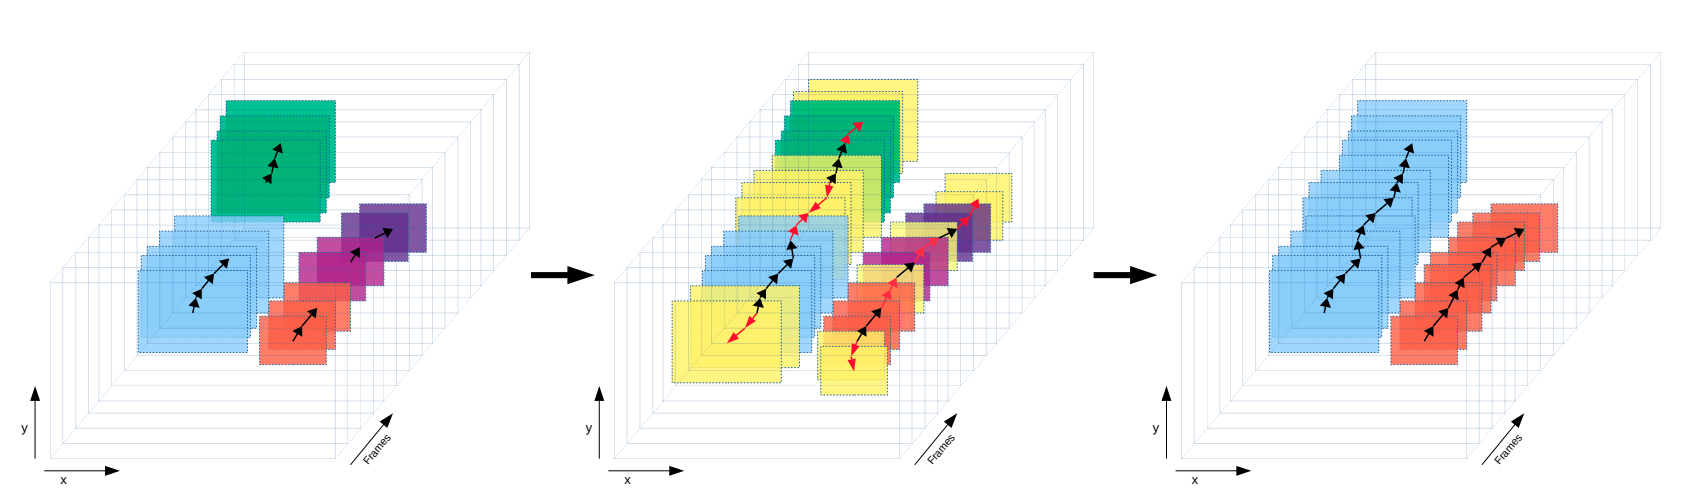
\includegraphics[width=\textwidth]{./imgs/visual_tracking.png}
	\caption{V-IoU Tracker追踪算法基本原理示意图。IoU tracker 方法经常因中间帧的漏检而导致过多的零碎轨迹片段(如左图所示),而这些中间帧的漏检可以通过使用一个视觉追踪模块进行补偿(中间图中黄色框为补偿的漏检框),从而生成片段数更少,连续性更强的轨迹\cite{bochinski2018extending}。}
	\label{fig:visual_tracking}
\end{figure}


目前多目标跟踪算法基本使用现有的检测模型得到所有帧的检测结果,然后设计数据关联算法得到多目标跟踪结果。例如SORT\cite{bewley2016simple}使用Faster-RCNN\cite{ren2015faster}作为目标检测器得到检测结果,然后使用中心坐标、面积、长宽比等对目标运动进行建模,使用卡尔曼滤波预测目标的后续状态,并将预测结果与实际结果进行匹配从而得到最终结果。在此基础上,作者又使用了深度卷积神经网络提取目标特征作为匹配基础改进SORT,从而得到DeepSORT[\cite{wojke2017simple}。此外,还有一种比较简单的,使用前后两帧各目标框的IoU进行关联的匹配算法IoU Tracker\cite{bochinski2017high},该算法严重依赖于检测框的准确率。为了改善对检测结果精度的依赖,作者之后推出了改进版V-IoU Tracker\cite{bochinski2018extending},该算法加入了检测框的长程连续性特征,当前没有检测出新目标的轨迹不再认为立即终止,而是会根据其运动趋势保持更新一定时间步长。如图\ref{fig:visual_tracking}所示,V-IoU Tracker算法通过在原来IoU Tracker算法的基础上增加了一个视觉追踪模块,补偿了中间帧漏检的目标,增加了轨迹的长程连续性。

\begin{algorithm}[!t]
	\caption{改进版 V-IoU Tracker 算法}
	\label{alg:viou-tracker}
	\textbf{输入: }$D=\{D_0,D_1,...,D_{F-1}\} = \{\{d_0, d_1, ..., d_{N_0}\},..., \{d_0, d_1, ..., d_{N_{F-1}}\}\}$\\
	\textbf{初始化:} $T_a=\phi,T_f=\phi, D = \{\{D_i \mid d_i \in D_j, d_j \leq \sigma_{low}\} \mid D_j \in D\}$
	
	\For{$f=0$ to $F$}
	{
		\For{$t_i\in T_a$}
		{
			$d_{best} = d_j$ where $\max(IoU(d_j, t_i)), d_j \in D_f$\\
			\If{$IoU(d_{best},t_i)\geq \sigma_{iou}$}
			{
				使用线性插值生成检测框以替代$t_i$中的虚拟占位框\\
				将$d_{best}$ 添加到 $t_i$,并将 $d_{best}$ 从 $D_f$ 中移除\\
			}
			\ElseIf{$t_i$ 中的虚拟占位框个数小于 $ttl$}{
				将一个新的虚拟占位框添加到$t_i$末尾
			}
			\ElseIf{$highest\_score (t_i) \geq \sigma_{high}$ 并且 $len(t_i)\geq t_{min}$}
			{
				移除$t_i$中的所有虚拟占位框\\
				将 $t_i$ 添加到 $T_f$,并将 $t_i$ 从 $T_a$ 中移除\\
			}
		}
		\For{$d_{j} \in D_f$}
		{
			以$d_j$为起点开始一段新轨迹$t$,并将$t$添加到$T_a$
		}
	}
	\For{$t_j\in T_a$}
	{
		移除$t_j$中的所有虚拟占位框\\
		\If{$highest\_score (t_j) \geq \sigma_{high}$ 并且 $len(t_j)\geq t_{min}$}
		{	
			将 $t_i$ 添加到 $T_f$
		}
	}
	\Return{$T_f$}
\end{algorithm}

V-IoU Tracker算法的具体流程如算法\ref{alg:viou-tracker}所示,其中,$D_f$是当前帧$f$的检测结果集合,$d_j$是$f$中第$j$个检测框,$T_a$为当前还在跟踪的轨迹集合,$T_f$为已经终止的轨迹,$F$是视频序列中帧的总数,$ttl$为允许添加的虚拟占位框的总个数。输入所有帧的检测结果,算法首先过滤掉置信度低于$\sigma_{low}$的检测框,然后对于当前激活的轨迹集合$T_a$中的每一条轨迹$t_i$,如果$t_i$能够根据当前帧找到与其末尾检测框IoU大于$\sigma_{iou}$的预测框,则直接将该预测框添加到$t_i$末尾,并将$t_i$中的虚拟占位框都用插值算法替换为预测框,否则则在$t_i$末尾添加一个虚拟占位框。如果$t_i$中的虚拟占位框个数大于$ttl$,则轨迹$t_i$就被视为已经终止,删除$t_i$中的虚拟占位框,经过轨迹置信度以及长度的筛选后,将其添加到$T_f$中。否则,如果虚拟占位框的个数不超过$ttl$,则继续追踪。虚拟占位框可以补偿由于漏检造成的轨迹中断,从而减少目标跟踪的零碎片段数。本工作的多目标追踪算法借鉴了该思路,只是将2D IoU 计算换成了3D IoU。


多目标跟踪的性能评价指标和单目标跟踪有很大不同,当前学术界最常使用的衡量指标为CLEAR MOT\cite{bernardin2008evaluating}论文提出的多目标追踪准确度(Multiole Object Tracking Accuracy,MOTA)和多目标追踪精确度(Multiple Object Tracking Precision,MOTP)。其中MOTA的计算公式如\ref{con:mota}所示,其中$t$表示帧数,$m_t, fp_t, mme_t$分别是$t$帧时漏检、误检以及错误匹配的数量,$g_t$为$t$帧中的真实标签。从公式可以看出MOTA可以分为三部分,$\overline{m}$为漏检率,$\overline{fp}$为误检率,$\overline{mme}$为错误匹配率,这三种错误率的总和就是总错误率。MOTA直观的给出了衡量算法连续跟踪识别目标的能力,不过没有涉及到目标的检测位置精确度。
\begin{equation}
\begin{split}
MOTA & = 1 - (\overline{m} + \overline{fp} + \overline{mme})\\
& = 1 - \left(\frac{\sum_t m_t}{\sum_t g_t} + \frac{\sum_t fp_t}{\sum_t g_t} + \frac{\sum_t mme_t}{\sum_t g_t} \right)\\
& = 1 - \frac{\sum_t (m_t + fp_t + mme_t)}{\sum_t g_t}
\end{split}
\label{con:mota}
\end{equation}
另一个指标MOTP与MOTA互补,其衡量跟踪目标位置的精确度,而不衡量跟踪识别目标的能力。MOTP的计算公式如\ref{con:motp}所示,其中$t$表示帧数,$i$表示第$t$帧第$i$个目标-预测匹配对,$d^i_t$表示第$t$帧中第$i$个目标-预测匹配对的位置误差,$c_t$表示第$t$帧中总匹配对的个数。在计算MOTA和MOTP时,都是基于整个跟踪过程计算平均值的,而不是基于每一帧的结果,这是因为基于单帧计算然后再求平均会导致和直观上不同的结果。
\begin{equation}
MOTP = \frac{\sum_{i,t} d^i_t}{\sum_t c_t}
\label{con:motp}
\end{equation}

除了MOTA与MOTP,为了更好的在轨迹层面上衡量多目标追踪,学术界一般还会引入其他指标。例如多数追踪率(Mostly Tracked,MT)、多数丢失率(Mostly Lost,ML)、ID切换次数(ID-switches,IDS)、片段数(Fragmentations,FM)。其中MT表示目标的大部分被追踪到的轨迹占比(大于80\%),ML表示目标的大部分跟丢的轨迹占比(小与20\%),IDS为跟踪轨迹改变目标编号的次数,FM为真实轨迹被打断的次数。本工作使用MOTA、MOTP以及以上四种指标评估多目标跟踪算法的性能。

\section{本章总结}
\label{tech_conclusion}
本章主要介绍了本文涉及到的两个领域,目标检测与目标跟踪的基本技术原理。首先介绍了两类目标检测框架的网络结构和训练方法,其中两阶段目标检测以Faster-RCNN作为代表进行介绍,而单阶段目标检测则以YOLO为代表进行介绍。之后,本章简单介绍了单目标跟踪算法的实现思路和几种经典算法。本章最后介绍了多目标跟踪的实现方式和几种典型算法,以及多目标追踪性能的评价指标。该章的内容是为下一章中本工作方法介绍的时候提供技术参考,本章涉及到的技术原理,下章将不再深入介绍。

% 打印时插入必要的空白页
\ifprint
	\newpage
	\thispagestyle{empty}
	\mbox{}
	
	% 避免空白页影响页码编号
	\clearpage
	\setcounter{page}{10}
\fi
	% !Mode:: "TeX:UTF-8"

\chapter{流数据的三维目标检测与跟踪}
\label{methodology}
本章将详细介绍本工作提出的流数据三维目标检测与跟踪框架 \textbf{DODT} (\textbf{D}ual-way \textbf{O}bject \textbf{D}etection and \textbf{T}racking)。本章先介绍DODT的整体网络架构,然后再重点分析各个模块的功能以及实现。

\section{框架整体结构}
\label{total_structure}
\begin{figure}[h]
	%\vspace{-0.3cm}
	\begin{center}
		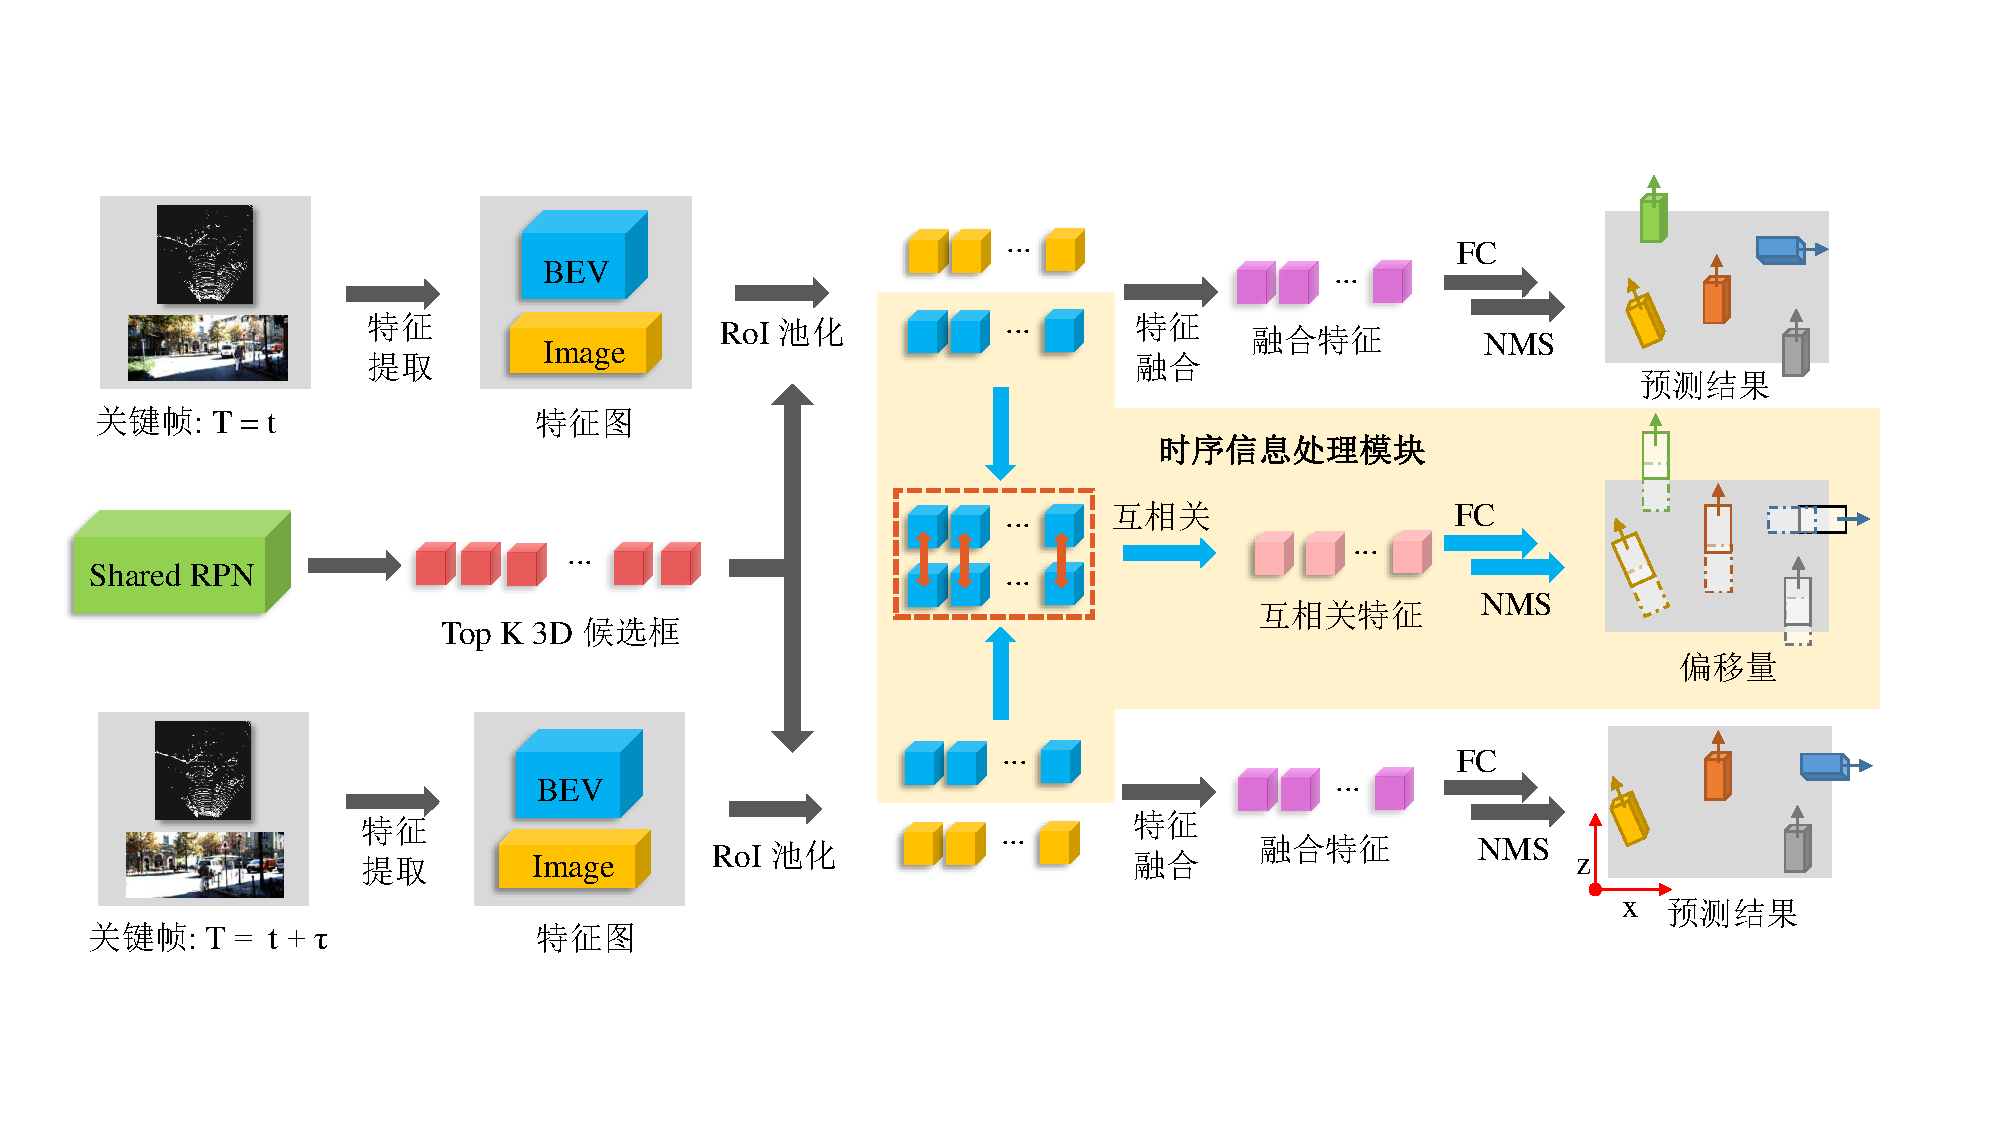
\includegraphics[trim={1.1cm, 2.5cm, 1.5cm, 2.5cm}, clip, width=\textwidth]{imgs/structure_final.pdf}
	\end{center}
	\vspace{-0.8cm}
	\caption{DODT 框架结构,FC表示全连接层,NMS是非极大值抑制过程。}
	\label{fig:dodt}
	%\vspace{-0.3cm}
\end{figure}


DODT网络是双路结构,其结构如\figurename \, \ref{fig:dodt} 所示。DODT由四个小模块组成:三维物体检测模块、Shared RPN模块、时序信息处理模块以及运动插值模块。三维物体检测模块有两个分支,分别负责检测两相邻关键帧中的物体,两分支的网络结构相同,并且共享参数。检测模块的网络结构是基于AVOD\cite{ku2018joint}构建的,为二阶段物体检测框架的三维扩展,该模块的详细结构将在3.2节介绍。Shared RPN 模块负责生成二阶段物体检测中的候选框,与传统RPN不同的是,Shared RPN生成的3D候选框可以被两个三维检测分支共同使用,该模块将在3.3节详细介绍。时序处理模块为 \figurename \, \ref{fig:dodt} 的浅黄色区域,该模块通过对相邻关键帧的点云俯视图(Bird Eye View,BEV)特征匹配块进行相关(correlation) 操作提取帧间的时序信息,然后预测同一物体物体在两关键帧的位置位置偏移。3.4节将详细介绍时序处理模块的实现原理。运动插值模块主要是由独立于网络结构的运动插值算法构成,该算法使用三维物体检测模块对两关键帧的检测结果以及时序处理模块输出的位置偏移信息,将关键帧的检测结果传播到非关键帧,实现流数据的三维物体检测与追踪。该算法的详细流程将会在3.5节重点介绍。


\section{三维物体检测模块}
\label{3d_detection_module}

DODT框架的三维物体检测模块融合了点云与图像信息,预测自动驾驶场景中车辆的三维位姿信息。由于该检测模块是基于AVOD\cite{ku2018joint}网络,为二阶段物体检测模块,因此包含候选框提取网络。由于本框架的候选框提取网络与AVOD有所不同,因此将在下一节详细介绍。本节不展开介绍候选框提取环节。本节将依次介绍数据预处理、特征提取、RoI池化、特征融合以及最终的预测框生成等物体检测中的关键步骤。

\subsection{数据预处理}

DODT融合RGB图像数据以及激光雷达数据进行三维物体检测,因此每一帧数据都同时包含图像以及点云。RGB图像数据预处理比较简单,首先统一调整长宽到$1200 \times 360 $ px,然后在RGB通道上将去数据集的RGB平均值$[R_{mean},G_{mean},B_{mean}]$(本工作基于的KITTI下的物体追踪数据集,RGB平均值为[92.84,97.80,93.58])。RGB图像数据经过色彩均值归一化后就可以直接用于后续的特征提取操作了。

点云数据的预处理相对于图像要更为复杂,这是因为点云是稀疏的三维数据,需要经过额外的操作将其转换为网络能够处理的形式。本工作采用网格化的方法将点云数据编码成六通道的BEV特征图,特征图包含五个高度切片通道以及一个点云密度信息通道。我们首先将点云投影到相机平面,然后过滤落在图像尺寸之外的点以便让点云视野与图像视野相同【TODO】。对于截取得到的规则三维视野,我们首先使用0.1m分辨率的网格将XZ平面网格化。假设XZ平面尺寸为 $[-W,W] \times [0, L] m$,则网格化后的尺寸为$\frac{2W}{0.1} \times \frac{L}{0.1}$。对于高度Y方向,我们截取$[0,2.5] m$ 的区域,然后平均切片为五等份从而将整个点云体素化。而后,将每个体素格子中所有点高度的最大值作为该格子的值,从而将点云编码为BEV特征图。对于特征图的最后一个通道,我们使用高度切片前的每个格子内的点计算该格子的点云密度 $\rho = \min(1.0, \frac{\log(N+1)}{\log 16})$,其中$N$为格子内点的数目。该方法最先在MV3D\cite{chen2017multi}中使用,而后AVOD\cite{ku2018joint}也使用了相同的处理方式。

在自动驾驶场景中,车辆是不停运动的,因此流数据中每一帧数据的参考系也不同。为了更好的关联帧与帧之间的时序信息,除了对每一帧数据进行预处理外,还需将不同帧的数据校准到同一坐标系。DODT为双路结构,同时处理相邻两帧关键帧数据并关联帧间信息。因此,为了统一两帧数据的坐标系,我们将后一帧关键帧数据校准到前一帧数据的坐标系中。由于图像数据没有准确的三维坐标信息,我们只校准点云数据。点云数据的校准需要用到激光雷达的位姿信息,这些数据KITTI数据集有提供。

\subsection{特征提取}

\begin{figure}
	%\vspace{-0.5cm}
	\centering
	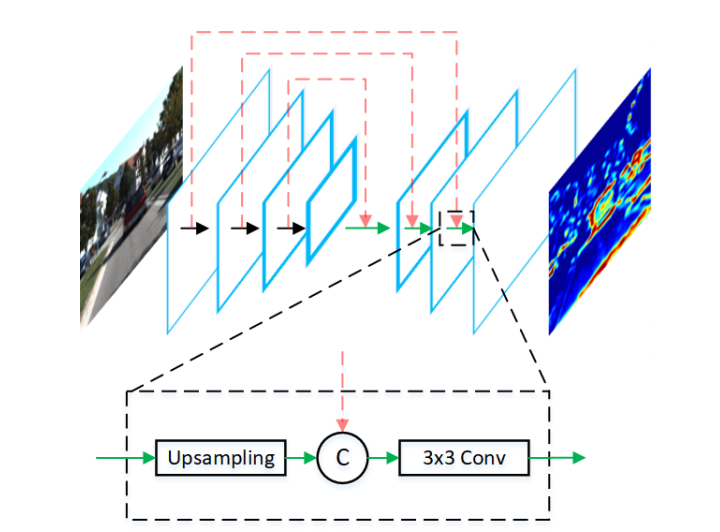
\includegraphics[width=0.8\textwidth]{imgs/feature-extractor.png}
	%\vspace{-0.3cm}
	\caption{特征提取网络结构。}
	\label{fig:feature_extractor}
	%\vspace{-1.5cm}
\end{figure}


DODT检测模块有两个单独的特征提取网络,分别用于图像特征提取以及点云特征提取。这两个网络的结构类似,只是输入的尺寸不一样。特征提取网络采用的编码器-解码器(Encoder-Decoder)结构,包含了编码器和解码器两部分,如\figurename \ref{fig:feature_extractor} 所示。编码器基于VGG-16网络改造的,首先将网络的通道数减半,并在conv-4层截断。编码器输入尺寸为 $M \times N \times D$ 的图像数据或是点云BEV特征图,然后输出尺寸为 $\frac{M}{8} \times \frac{N}{8} \times D^*$ 的特征$F$。特征$F$能够表达高层次的语意信息,并且尺寸比输入小了八倍。KITTI数据集中行人在BEV视角平均大小为$0.8 \times 0.6$ 米,在BEV特征图上就是$8 \times 6$ 的像素区域(分辨率为0.1m)。在编码器八倍下采样后,行人在输出特征$F$中占据不到一个像素,这还是在不考虑卷积过程中感受野的放大所造成小物体占比缩小的情况。受特征金字塔网络(Feature Pyramid Network)的启发,AVOD设计了一个自底向上的解码器,解码器可以在几乎不增加运行时间的基础上,将特征$F$上采样到输入的尺寸大小。解码器将编码器的输出作为输入,然后生成尺寸为$M \times N \times D$ 的特征图。解码器的上采样是通过反卷积算子实现的,为了更好的补回编码器中下采样造成的细节损失,解码器每一层的输入还额外包含编码器对应层的特征,然后通过一个$3 \times 3$的卷积操作融合。最终的特征图在保留了对高层语意的表征能力下,还能有与输入相同的尺寸,这在一定程度上避免了小物体特征丢失的问题。

\subsection{特征融合}

\begin{figure}[t]
	\centering
	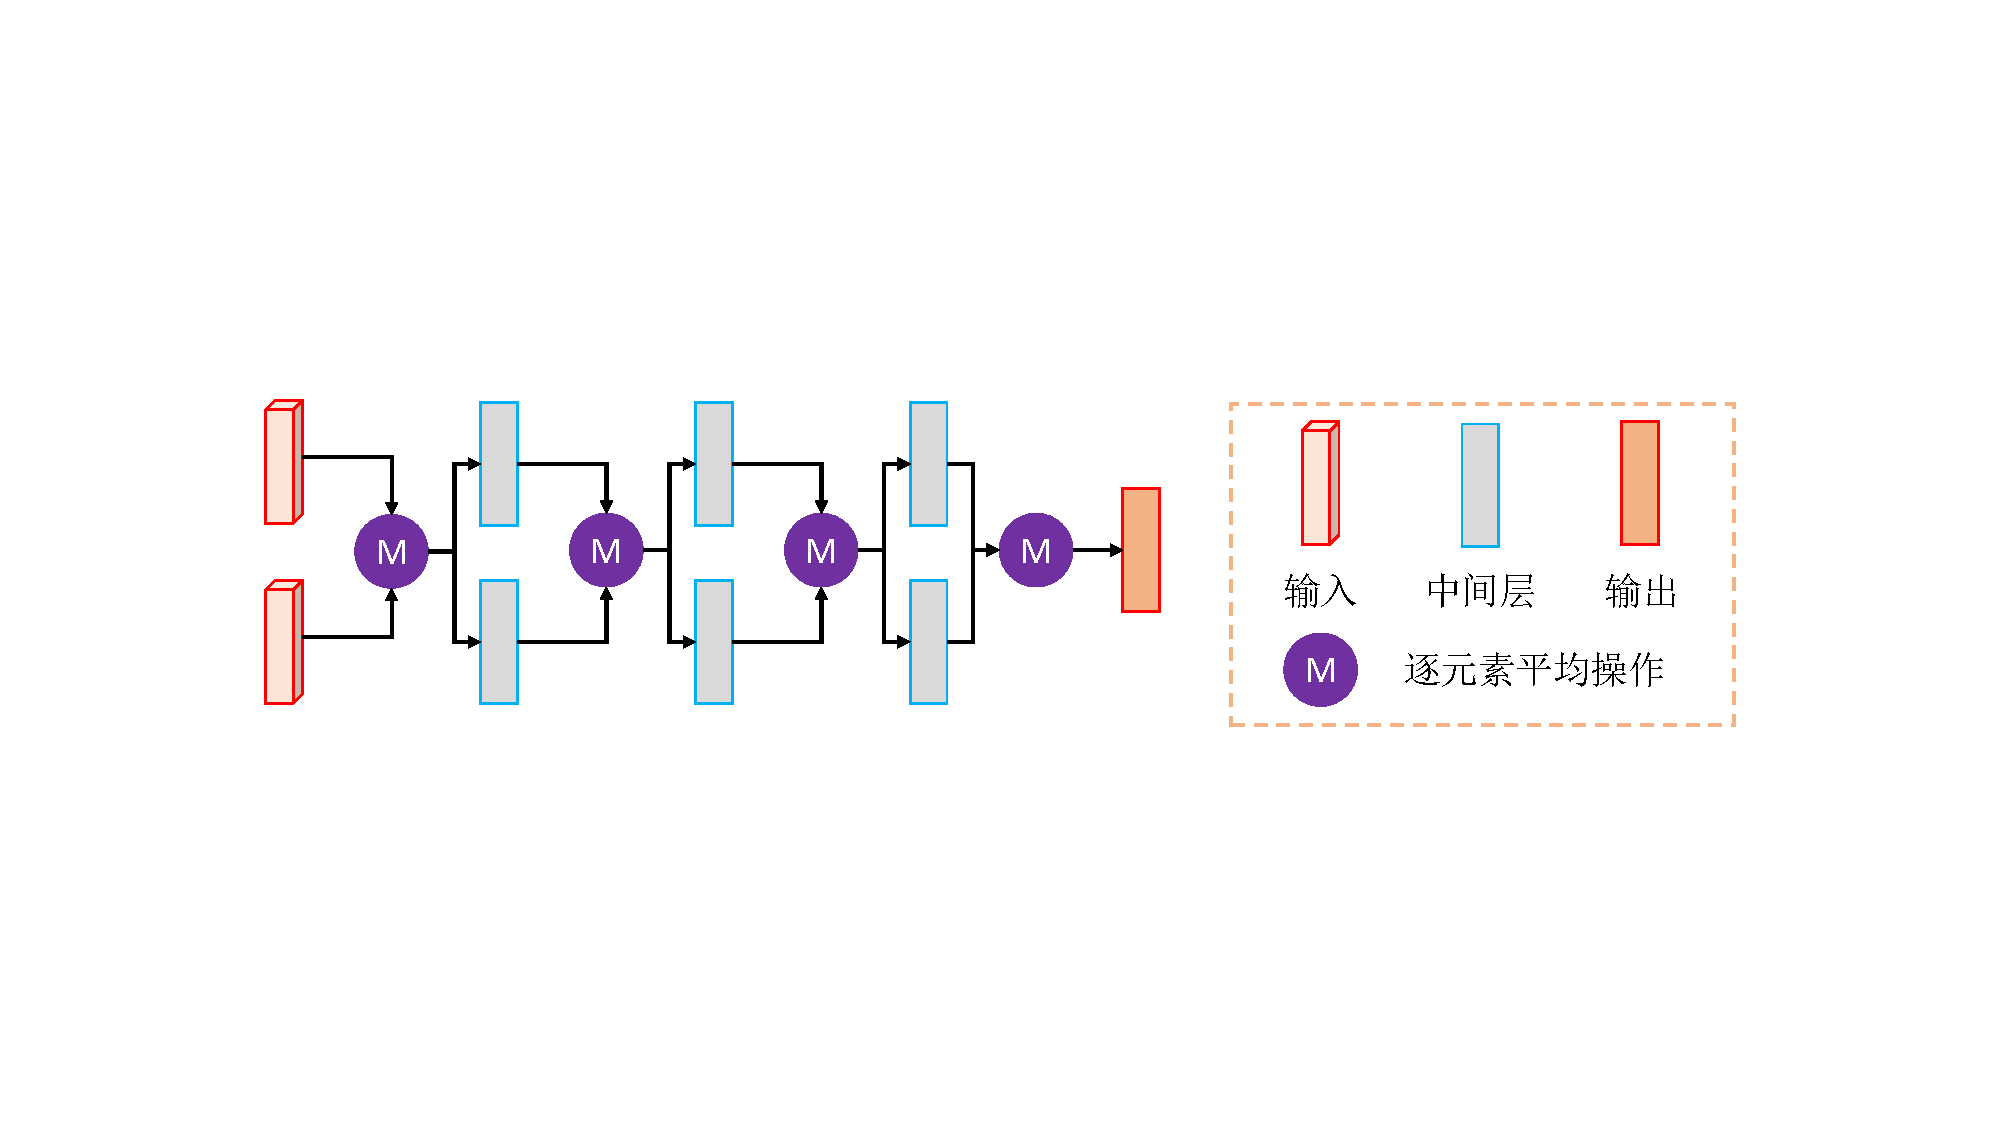
\includegraphics[trim={4cm, 6cm, 4cm, 6cm}, clip, width=\textwidth]{imgs/fusion-network.pdf}
	\caption{深度融合网络(deep fusion)结构,输入为点云BEV特征$f_{img}$以及图像特征$f_{pc}$。}
	\label{fig:fusion_network}
\end{figure}


在特征提取阶段我们分别得到了图像的特征$F_{img}$以及点云的特征$F_{pc}$,接下来就是将这两种特征融合以得到更丰富的视觉特征。DODT的特征融合也是借鉴了AVOD的方式,在候选框层面上进行融合。给定一个3D候选框由(Shared RPN生成),将其投影到$F_{img}$以及$F_{pc}$上,截取相应的部分就能得到对应的候选区域特征$f_{img}$ 以及$f_{pc}$。之后$f_{img}$ 和 $f_{pc}$ 将会通过$7 \times 7$的ROI池化操作生成相同尺寸的特征向量,之后两特征向量通过一个融合网络生成最终的候选区域特征向量$F_{fusion}$。融合网络结构如\figurename \ref{fig:fusion_network} 所示,该网络结构最先由MV3D提出,叫做深度融合网络。对于有$L$层的网络,深度融合网络按如下方式融合特征:
\begin{equation}
	\begin{aligned}
		& F_0 = F_{img} \oplus F_{pc}\\
		& F_l = H^{img}_l(F_{l-1}) \oplus H^{pc}_l(F_{l-1})\\
		& \forall l = 1, ..., L
	\end{aligned}
\label{con:deep_fusion}
\end{equation}
其中,$\{H_l, l=1,...,L\}$是特征转移函数(由神经网络拟合),$\oplus$为某种融合操作(例如拼接、求和等,DODT使用的是平均)。深度融合网络可以让两种特征能在更深层次、更高的语意层面进行融合,从而取得更好的融合效果。

\subsection{预测框生成}

\begin{figure}[t]
	\centering
	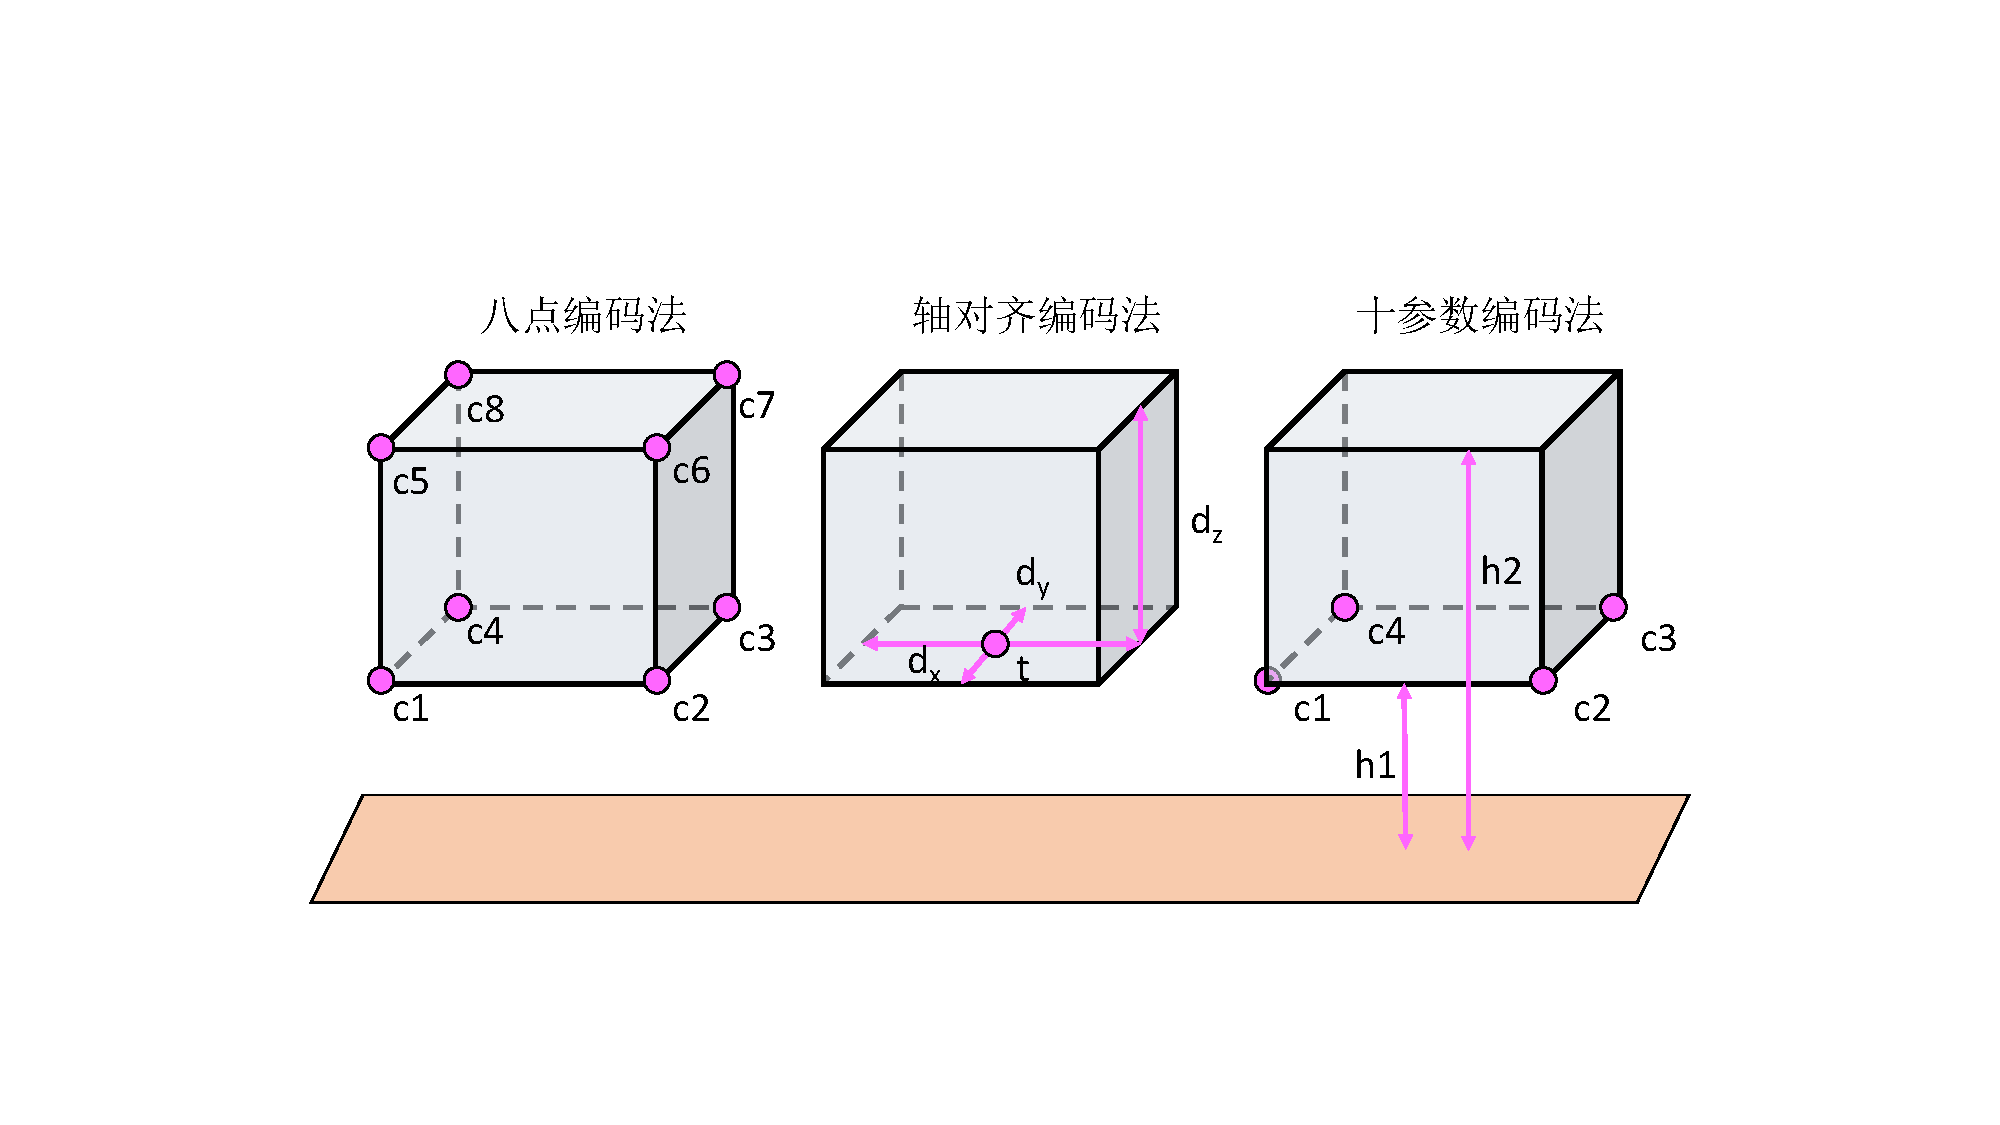
\includegraphics[trim={5cm, 3.5cm, 5cm, 4cm}, clip,width=\textwidth]{imgs/box-encoding.pdf}
	\caption{三种三维框编码方式。}
	\label{fig:box_encoding}
\end{figure}


特征融合之后,融合的特征图将会输入到两个不同任务分支,分别为检测分支和回归分支, 这两个分支都是由三层2048个神经元组成的全连接层。检测分支负责预测目标的类别,使用交叉熵计算损失值;而回归分支负责预测候选框与真实物体框的差值,使用$Smooth L1$ 函数计算损失值。在回归损失中,只有当候选框与真实框在BEV视角的 2D IoU 大于 0.65 才会被计算。之后, DODT使用NMS算法去除重叠的框,阈值设置为 0.01。

在框回归中,对三维框的编码有很多种方式,其中比较常见的有八点编码法和轴对齐(Axis Aligned) 编码法,如\figurename \ref{fig:box_encoding} 所示。八点编码法直接编码八个顶点的坐标,这种方式没有考虑三维框自身的几何约束,有一定的冗余性。而轴对齐编码限制了三维框要和坐标轴对齐,这是在RPN阶段使用的,并不适合最终的框编码。DODT使用了AVOD提出的10参数编码法,如\figurename \ref{fig:box_encoding}最右侧所示,分别编码底部四点坐标以及底面与顶面和地面的距离,一共有十个参数,因此框回归的目标为 $(\Delta_{x1}, ...,\Delta_{y1}, \Delta_{y4}, \Delta_{h1}, \Delta_{h2})$。这种编码方式考虑到了三维框顶面四点和底面四点是对齐的,而原来的过参数化的八点法需要编码成24维向量。

在MV3D中,作者默认三维预测框的朝向为长边方向,可是这种确定朝向的方法是有问题的。首先并不是所有目标都适用于这种确定朝向的方法,比如行人;其次,长边有两个可取的方向,它们相差 $\pm \pi$。AVOD中,作者通过预测转向向量 $(x_{\theta},y_{\theta}) = (\cos(\theta), \sin(\theta))$来解决这个问题。这种方式可以将每个转向角$\theta \in [-\pi, \pi]$都映射到唯一的转向向量。转向向量的预测也是包含在回归分支中。另外,转向向量可以用来解决十参数编码法中预测框与真实框底部四点的对应关系。底部四点的对应有四种,只使用十参数编码时只能通过最近匹配法,有了转向向量之后,转向向量的值可以作为额外的匹配手段。


\section{Shared RPN模块}
\label{shared_rpn}

\begin{figure}
	%\vspace{-0.5cm}
	\centering
	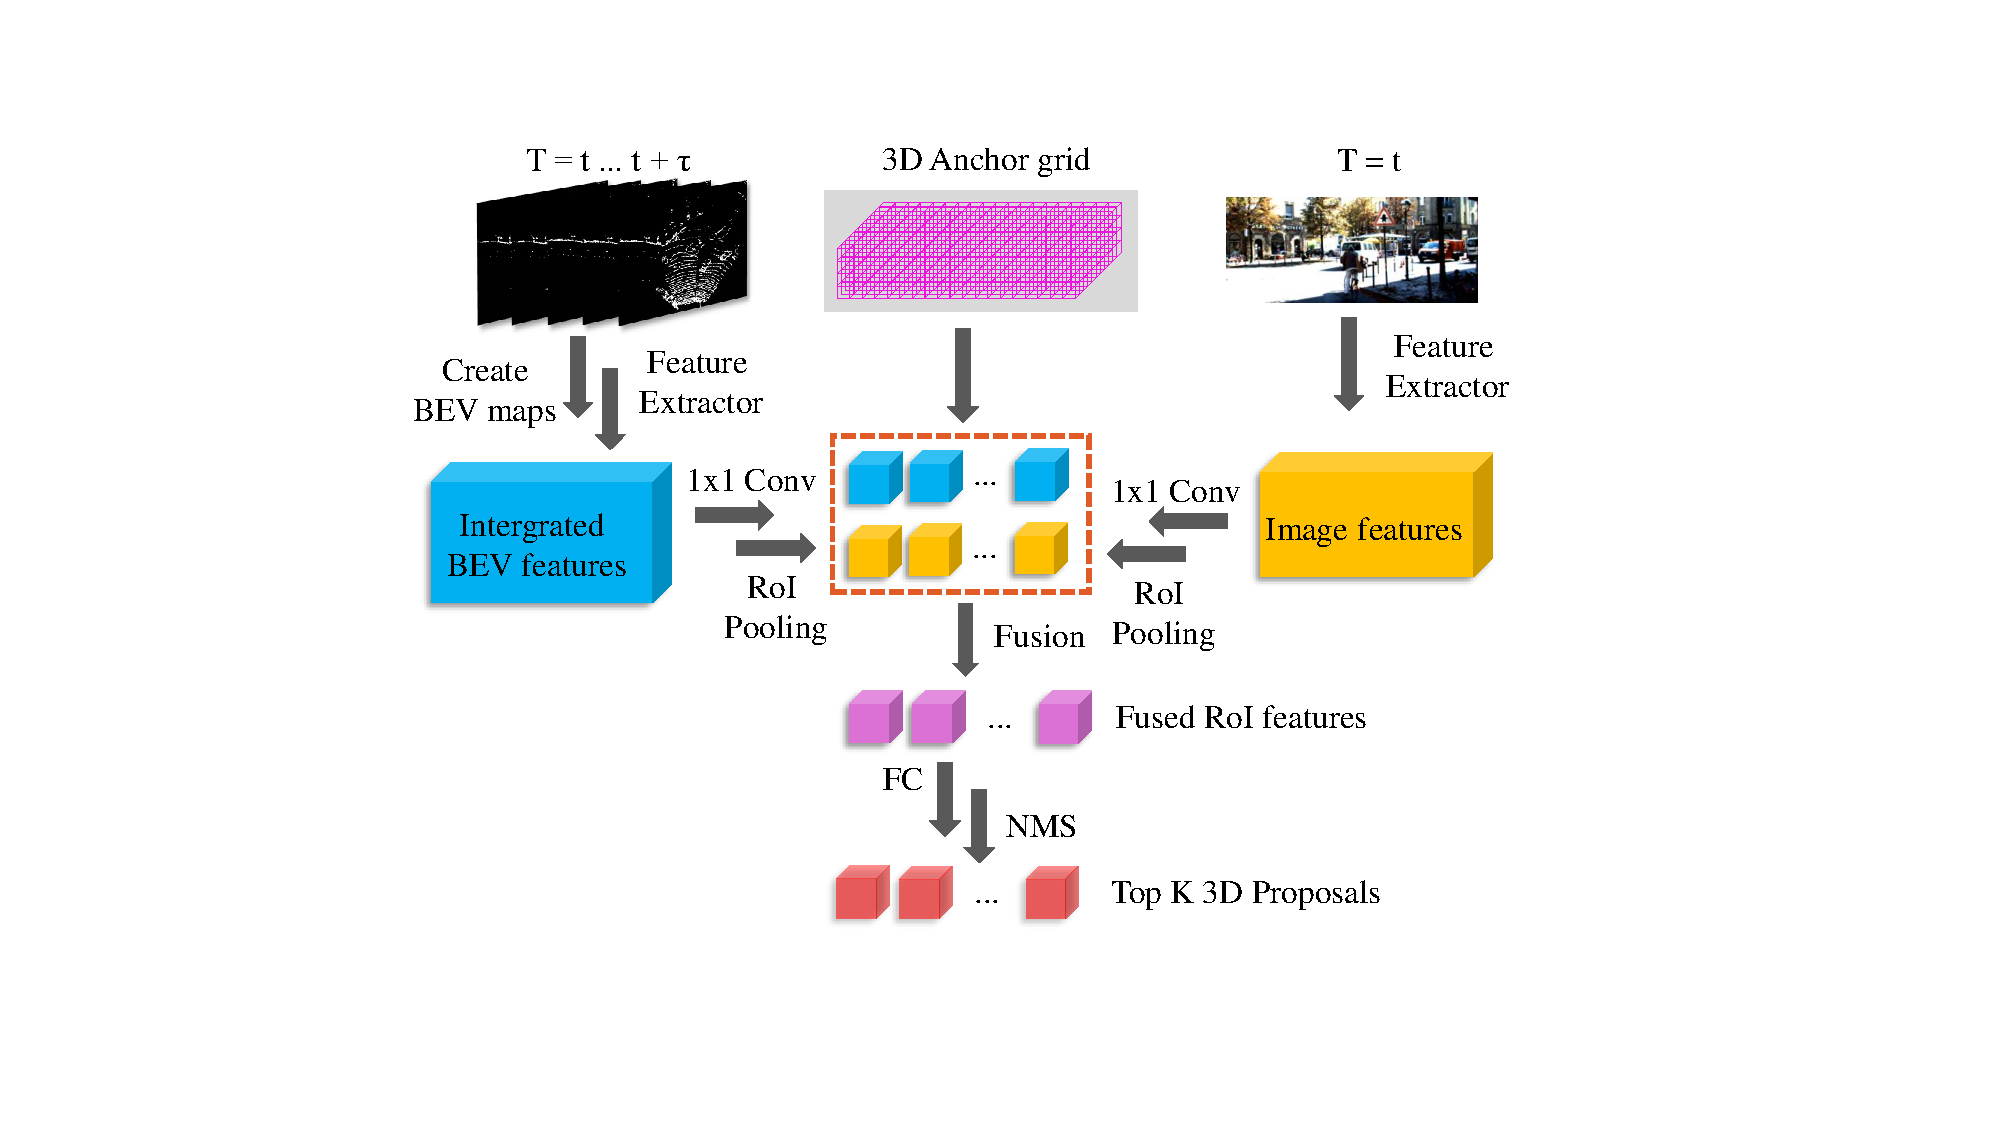
\includegraphics[trim={7cm, 3.5cm, 8cm, 2cm}, clip,width=0.8\textwidth]{imgs/rpn_final.pdf}
	%\vspace{-0.3cm}
	\caption{Shared RPN 模块。}
	\label{fig:shared_rpn}
	%\vspace{-1.5cm}
\end{figure}


\begin{figure}[t]
	\begin{center}
		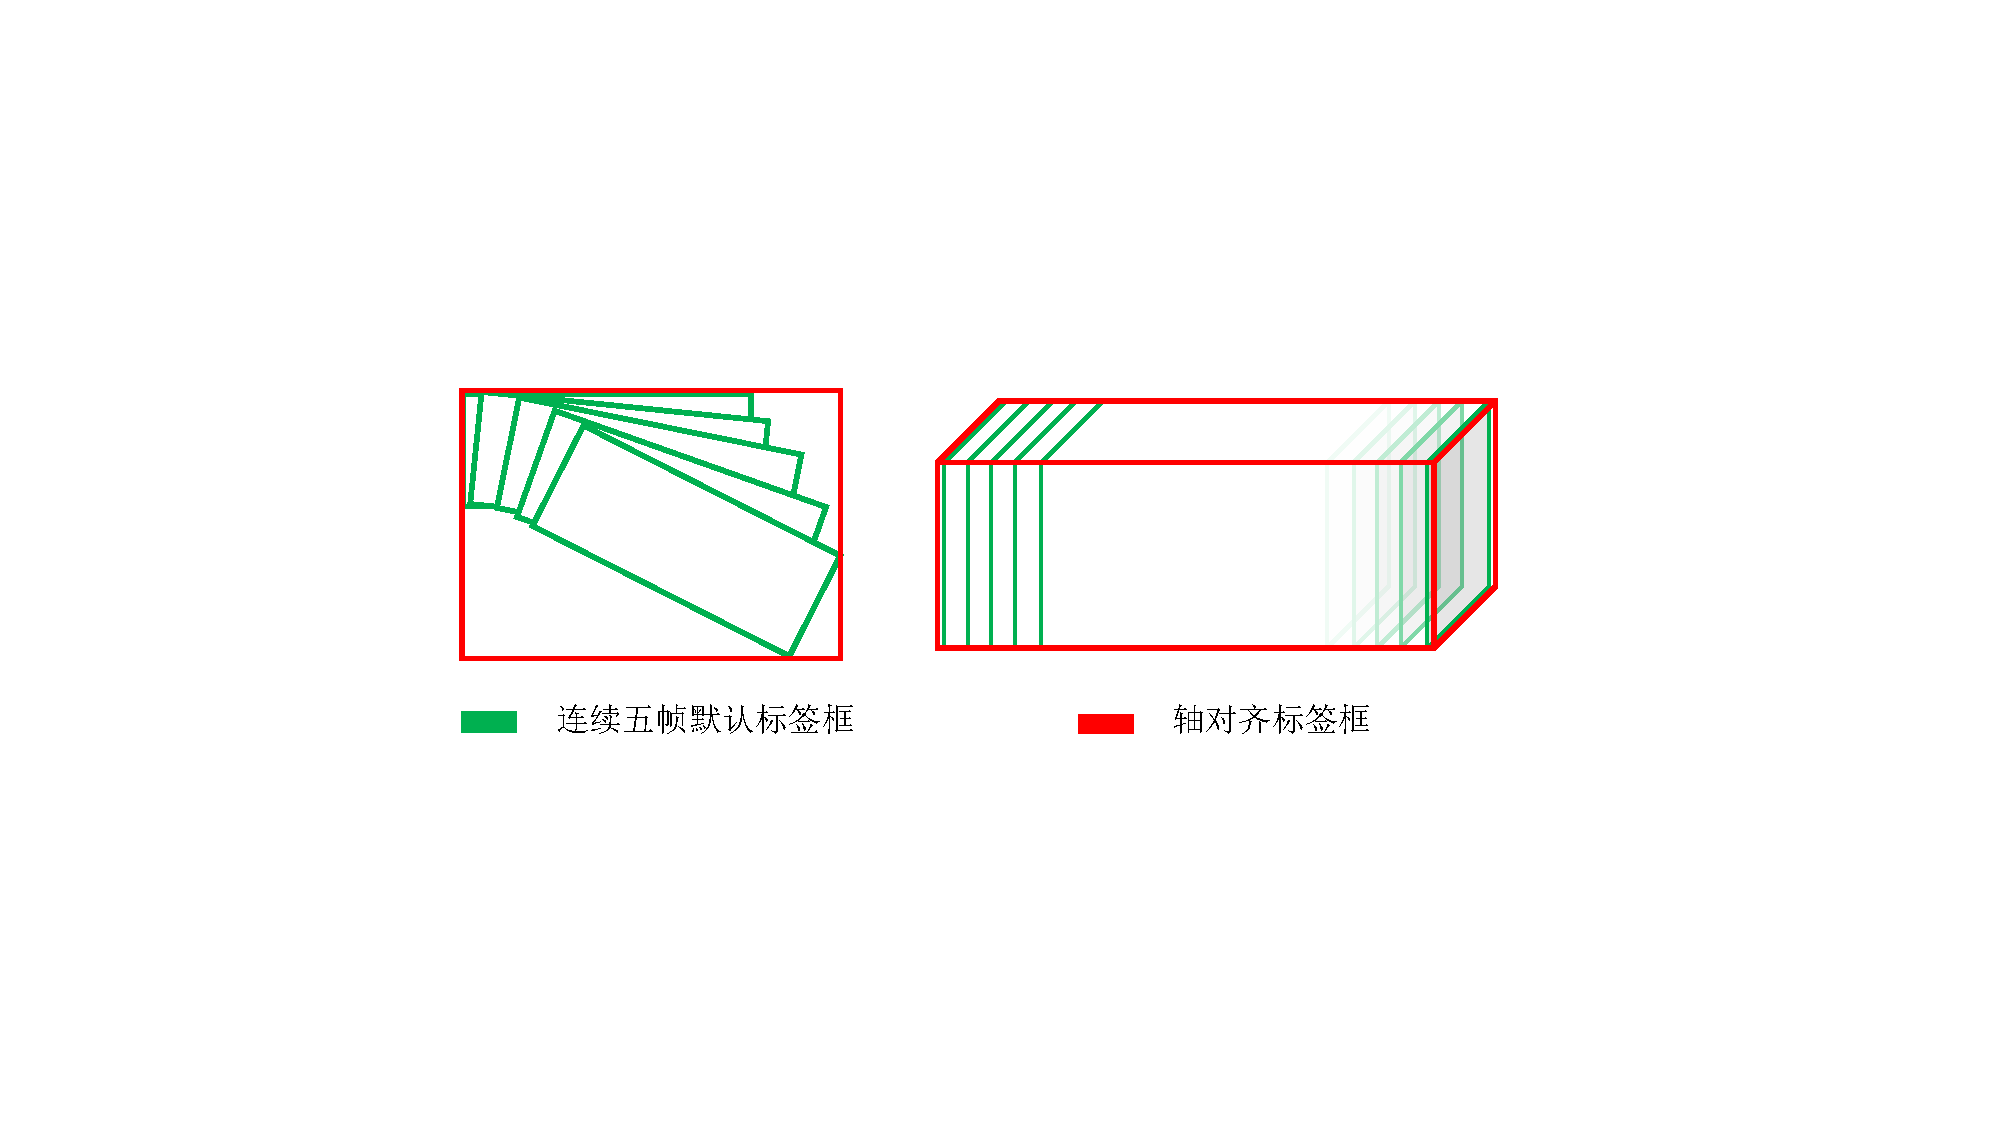
\includegraphics[trim={6cm, 6cm, 8cm, 6cm}, clip, width=0.8\textwidth]{imgs/axis-aligned-boxes.pdf}
	\end{center}
	\vspace{-0.8cm}
	\caption{\textcolor{green}{绿色} 框是五帧中目标的标签框,\textcolor{red}{红色}框是为训练\textit{Shared RPN} 而新生成的共享候选框标签。}
	\label{fig:integrated_boxes}
\end{figure}


\section{时序信息处理模块}
\label{temporal_module}

\begin{equation}
\delta^{t, t+\tau} = \\
\begin{cases}
(\frac{d_{x}^{t+\tau} - d_{x}^{t}}{d^t_{w}}, \frac{d_{z}^{t+\tau} - d_{z}^{t} }{d^t_{l}}, \frac{d_{ry}^{t+\tau} - d_{ry}^{t}}{d^t_{ry}}) & p_{co} = 1.0 \\
(0.0,0.0, 0.0) &  otherwise
\end{cases}
\end{equation}

\section{运动插值模块}
\label{interpolation}

\begin{algorithm}
	\caption{基于运动模型的插值算法(MoI Algorithm)}
	\label{alg:interpolation}
	\textbf{输入: } $D^t= [d^t_0, d^t_1, ..., d^t_{N_t}], D^{t+\tau}= [d^{t+\tau}_0, d^{t+\tau}_1, ..., d^{t+\tau}_{N_{t+\tau}}],$
	$\Delta^{t, t+\tau}=[\delta^{t, t+\tau}_0, \delta^{t, t+\tau}_1, ..., \delta^{t, t+\tau}_{N_{max}}], N_{max} = \max\{N_t, N_{t+\tau}\}$\\
	\textbf{输出: } $D = [D^t, D^{t+1}, ..., D^{t+\tau}]$\\
	\textbf{初始化:} $D_{temp} = D^{t+\tau}, D, p_{co}^{max} = 0.5$ \\
	\For{$d^t_i \emph{ in } D^t$}{
		$\Delta d^{t, t+ \tau}_{i} = (d^t_{i, w} \cdot \delta^{t, t+\tau}_{i,x}, 0, d^t_{i, l} \cdot \delta^{t, t+\tau}_{i,z}, 0, 0, d^t_{i, ry} \cdot \delta^{t, t+\tau}_{i,ry})$
		$d' = getMatched(d^t_i+\Delta d^{t, t+ \tau}_{i}, D_{temp})$\\
		\If{$d'$}{
			$d^{t+1}_i,..., d^{t+\tau-1}_i = Interpolate(d^t_i, d')$\\
			remove $d'$ from $D_{temp}$
		}
		\ElseIf{$p_{co}^i \geq p_{co}^{max}$}{
			$d^{t+1}_i,..., d^{t+\tau}_i = Interpolate(d^t_i, d^t_i + \Delta d^{t, t+ \tau}_{i})$
		}
		\Else{generate $(d^{t+1}_i,..., d^{t+\tau-1}_i)$ by motion model}
	}
	\If{$D_{temp}$ is not empty}{
		\For{$d^{t+\tau}_j \emph{ in } D_{temp}$}{
			\If{$p_{co}^j \geq p_{co}^{max}$}{
				$d^{t}_j,..., d^{t+\tau-1}_j = Interpolate(d^{t+\tau}_j - \Delta d^{t, t+ \tau}_{j}, d^{t+\tau}_j)$
			}
			\Else{
				generate $(d^{t+1}_j,..., d^{t+\tau-1}_j)$ by motion model
			}
		}
	}
\end{algorithm}



\section{多目标追踪}
\label{tracking_module}




\section{本章总结}
\label{metho_conclusion}

% 打印时插入必要的空白页
\ifprint
\newpage
\thispagestyle{empty}
\mbox{}

% 避免空白页影响页码编号
\clearpage
\setcounter{page}{10}
\fi
	% !Mode:: "TeX:UTF-8"

\chapter{实验过程与结果分析}
\label{experiment}
本章将介绍本项目的实验部分,包括对KITTI数据集、数据预处理、模型训练以及实验结果分析等内容。在结果分析中,我们首先比较DODT各模块对结果的影响,以考察每个模块的有效性;然后我们探讨了关键帧的选取步长对三维物体检测结果的影响,以便确定最优的步长;最后我们也测试了DODT在多目标追踪任务上的性能,并与前沿方法对比。结果显示DODT框架能很好的完成流数据的三维物体检测以及多目标跟踪任务。

\section{KITTI数据集介绍}
\label{kitti}
本项目的所有实验都是基于无人驾驶领域中广泛使用的KITTI公开数据集开展的。KITTI数据集是由德国卡尔斯鲁厄理工学院和丰田美国技术研究院联合采集的,该数据集包含多种传感器数据:一个惯性导航系统(GPS/IMU,型号为OXTS RT 3003)数据,一个激光雷达(Velodyne HDL-64E)数据,两个灰度相机数据(140万像素)以及两个彩色相机数据(140万像素)。其中激光雷达扫描频率为10帧/秒,相机基本与地平面保持平行,图像采集的尺寸为$1382 \times 512$像素。所有传感器的整体布局如\figurename \ref{fig:KITTI}。

\begin{figure}[h]
	\centering
	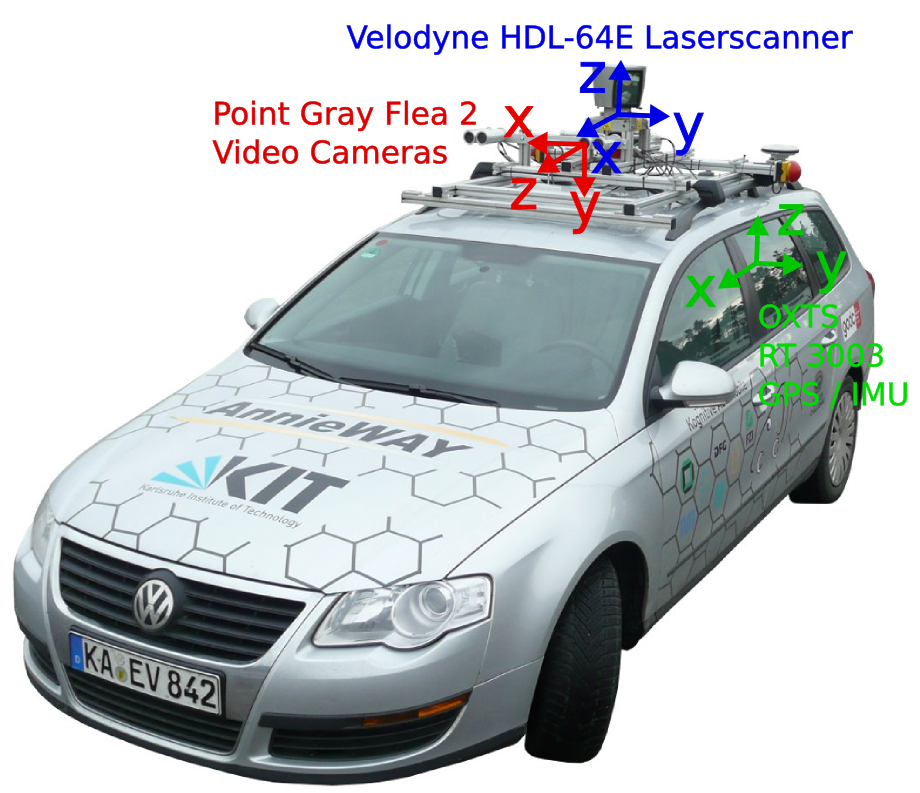
\includegraphics[width=0.6\textwidth]{./imgs/KITTI.png}
	\caption{KITTI数据集传感器整体布局。}
	\label{fig:KITTI}
\end{figure}

KITTI数据集根据不同的任务分为stero、flow、scenceflow、depth、odometry、object以及tracking等部分,对应着场景流估计、深度估计、路径规划、物体检测以及目标追踪等任务。每一个任务数据包都包含了海量的训练数据以及测试数据,供研究者使用。本项目主要使用了KITTI数据集的tracking数据包,该数据包由21段训练视频流(共8004帧数据)以及29段测试视频流(共11095帧数据)组成。每一段视频流都是由连续的RGB图像帧以及三维点云帧组成,在训练数据集中,还包含了每一帧数据对应的二维目标框(针对图像数据)以及三维目标框(针对点云数据)。此外,针对每一段视频流,KITTI还提供了传感器的标定信息以及每一帧的GPS/IMU数据,供研究者数据标定时使用。

多目标追踪的标签共有10项,记录了帧的信息以及帧中每个目标的信息。信息列举如下:
\begin{itemize}
	\item frame id:帧的编号;
	\item object id:每一帧中目标的编号,也是轨迹的编号;
	\item type:目标的类别,有”Car“,”Van“, "Trunk",”Pedestrian“,”Cyclist“等类别,本实验将”Car“和”Van“合并为”Car“类,并只针对”Car“类进行检测和追踪;
	\item truncated:标记目标是否被图像边界截断,”0“表示不截断,”1“表示截断;
	\item occluded:标记目标被遮挡的程度,共有0到3四个取值,”0“表示完全可视,”1“表示部分遮挡,”2“表示大部分遮挡,”3“表示完全遮挡;
	\item alpha:目标的观测角,$\alpha \in [-\pi, \pi]$;
	\item bbox:物体在图像上的2D边界框,包含左上角,右下角的坐标值;
	\item dimensions:物体的高、框和长,单位为米;
	\item location:物体底部中心点在相机坐标系的三维坐标 x,y,z,单位为米;
	\item ry:物体在相机坐标系沿Y轴的旋转角,$r_y \in [-pi, pi]$。
\end{itemize}
其中目标的观测角$\alpha = -[(\pi+r_y) + (\pi+\beta)]$,$r_y$与$\beta$如\figurename \ref{fig:kitti_obj}所示,而目标的location坐标如\figurename \ref{fig:kitti_box3d}所示。
\begin{figure}[!t]
	\centering
	\begin{minipage}[t]{0.5\textwidth}
		\centering
		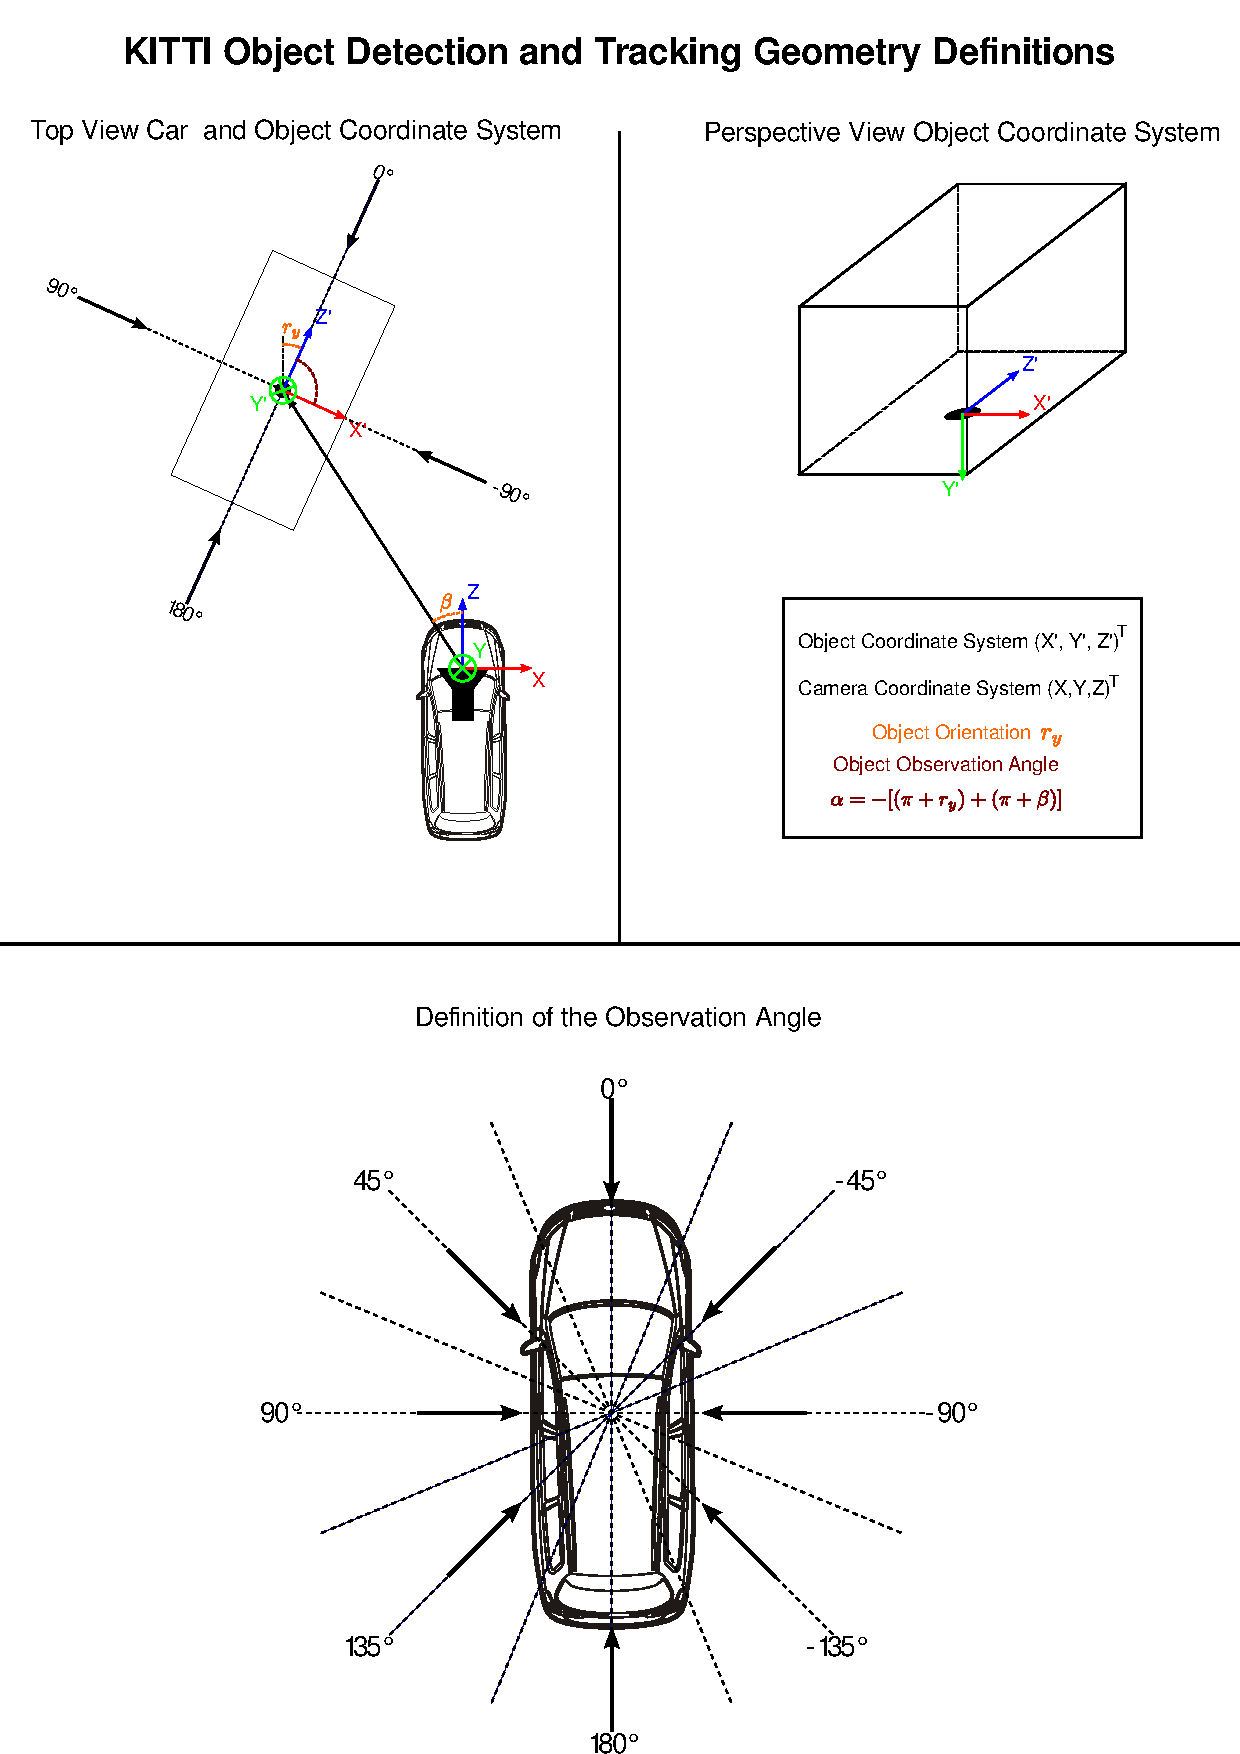
\includegraphics[trim={0cm, 15cm, 12cm, 2.5cm}, clip,width=\textwidth]{./imgs/KITTI_obj.pdf}
		\caption{KITTI数据集观测角与转向角示意图。}
		\label{fig:kitti_obj}
	\end{minipage}
	\begin{minipage}[t]{0.48\textwidth}
		\centering
		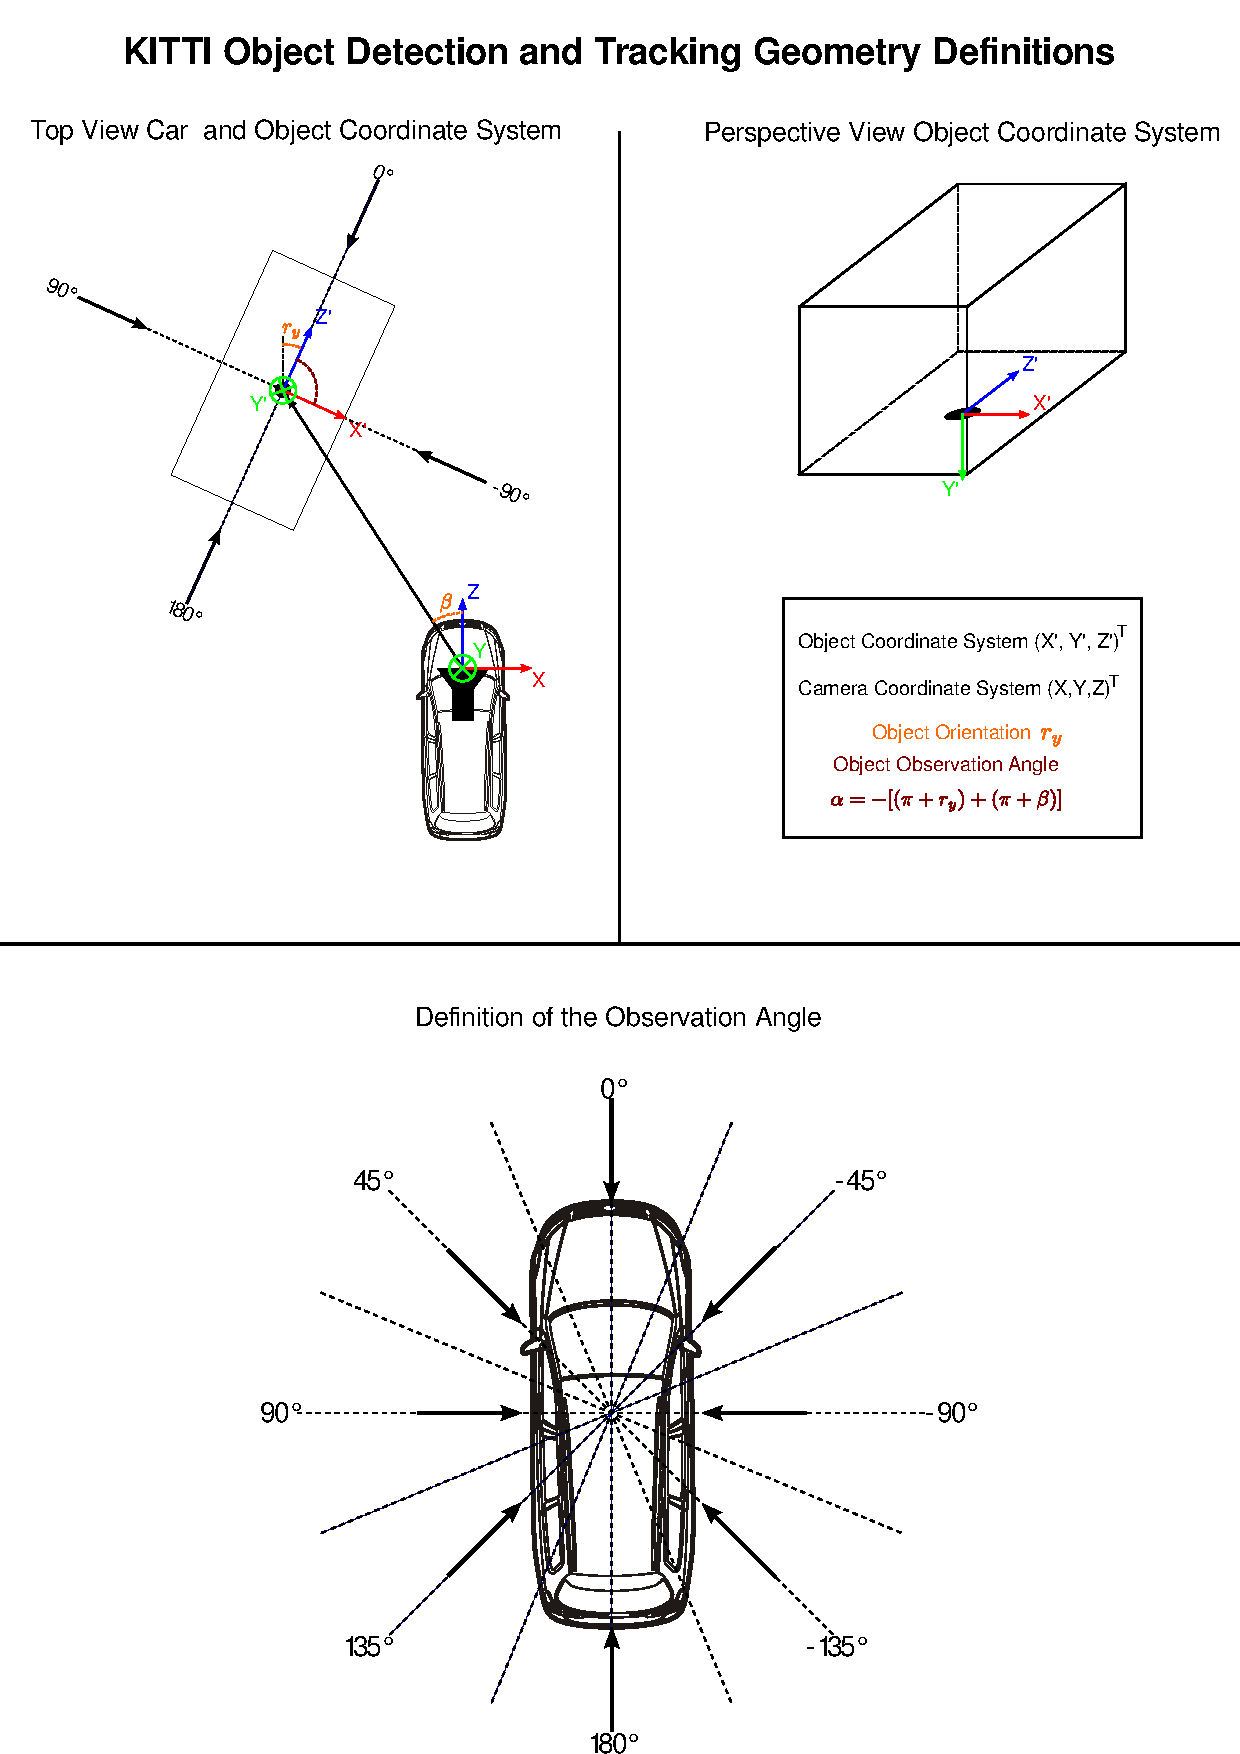
\includegraphics[trim={12cm, 20cm, 1.8cm, 2.5cm}, clip,width=\textwidth]{./imgs/KITTI_obj.pdf}
		\caption{KITTI数据集目标的位置坐标。}
		\label{fig:kitti_box3d}
	\end{minipage}
\end{figure}


传感器的标定信息保存在”calib.txt“文件中,其中包含了相机的参数矩阵以及各传感器之间的旋转矩阵。信息列举如下:
\begin{itemize}
	\item P0-P3:四个相机的内参矩阵 $P \in \mathcal{R}^{3\times 4}$;
	\item R0\_rect:$\mathcal{R}^{3\times 3}$,将摄像机坐标系转换到图像坐标系的校准矩阵;
	\item Tr\_velo\_to\_cam:$\mathcal{R}^{3\times 4}$,激光雷达坐标系到摄像机坐标系的旋转矩阵;
	\item Tr\_imu\_to\_velo:$\mathcal{R}^{3\times 4}$,IMU坐标系到激光雷达坐标系的旋转矩阵。
\end{itemize}

GPS/IMU数据提供了30项信息,其中包含每一帧中自身车辆的经纬度、海拔、三个欧拉角(roll,yaw以及pitch)、速度、加速度、角速度等信息。本实验主要使用到了经纬度以及欧拉角信息将不同帧之间的信息校准到同一坐标系。欧拉角包含了偏航角(yaw,表示机体轴在水平面上的投影与地轴之间的夹角,右偏为正)、俯仰角(pitch,表示机体轴与地平面之间的夹角,抬头为正) 以及翻滚角(roll,表示机体对称面绕机轴转动的角度,右滚为正),如\figurename \ref{fig:euler}所示。
\begin{figure}[t]
	\centering
	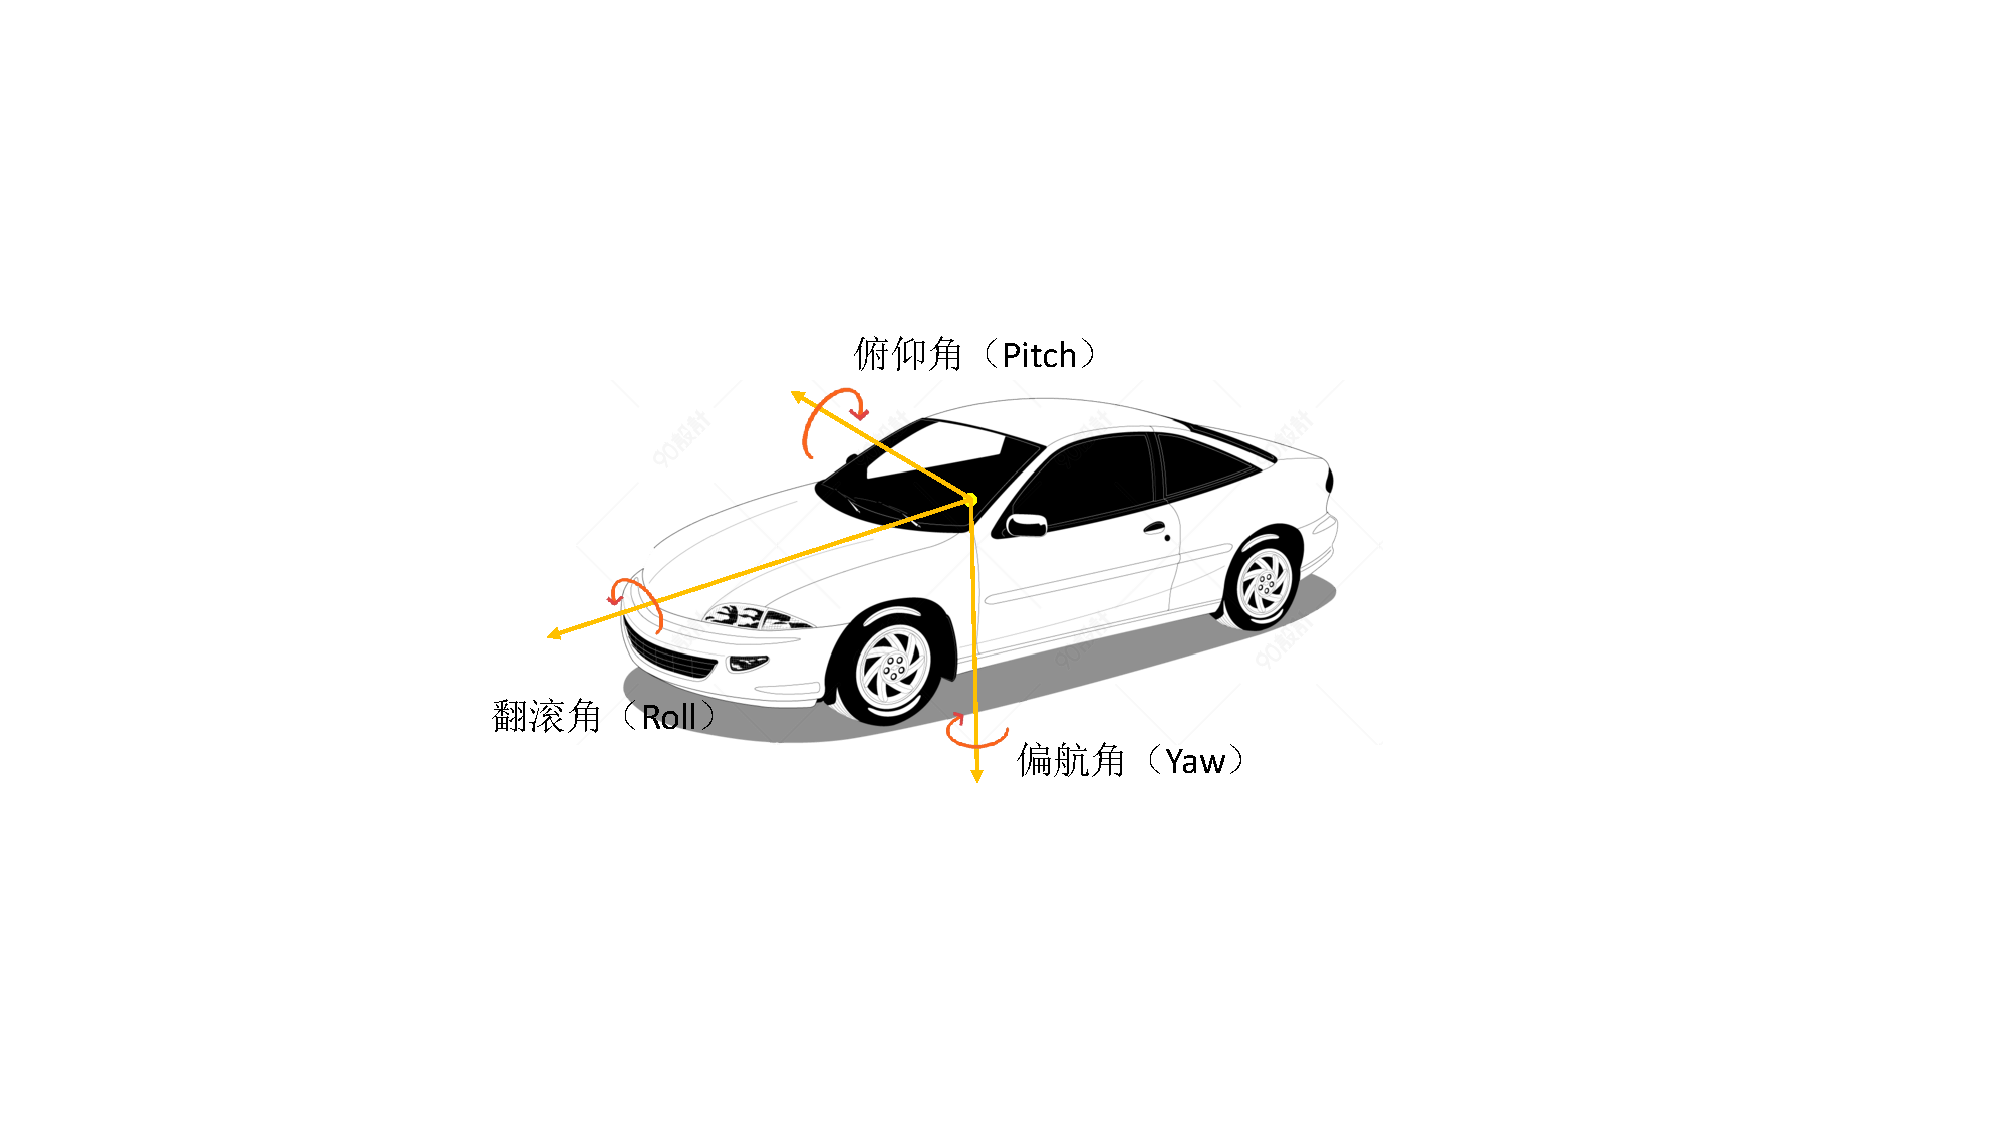
\includegraphics[trim={5cm, 6cm, 5cm, 5cm}, clip,width=\textwidth]{./imgs/euler.pdf}
	\caption{三个欧拉角的方向示意图。}
	\label{fig:euler}
\end{figure}



\section{数据预处理}
\label{preprocessing}


\section{模型训练}
\label{training}


\section{实验结果分析}
\label{results}


\subsection{三维物体检测结果分析}
\label{ablation_study}

\begin{table}[t]
	\centering
	\wuhao
	\caption{候选框预测性能比较。}
	\vspace{0.3cm}
	\begin{tabular}{ccc}
		\toprule[1.5pt]
		方法        & 原始 RPN & \textit{Shared RPN}  \\ \midrule
		准确率(\%)  & 97.81      & \textbf{98.47}       \\
		\bottomrule[1.5pt]
	\end{tabular}
	\label{table:rpn_result}
\end{table}


\begin{table}\centering
	\wuhao
	\caption{DODT的不同设置在验证数据集上的结果(只预测“Car”类别)。每项的指标为$AP_{3D}/AP_{BEV}$ (\%), 为三维物体检测在3D视角和BEV视角的平均精度。 “S” 表示\textit{Shared RPN}模块, “T” 表示时序信息处理模块, “M” 表示运动插值模块。 $\tau$ 是关键帧选取步长。} 
	\vspace{0.3cm}
	\resizebox{\textwidth}{!}{
		\begin{tabular}{ccccccccc}
			\toprule[1.5pt]
			&\multicolumn{1}{c|}{}   & \multicolumn{3}{c|}{IoU = 0.5}  		         & \multicolumn{3}{c|}{IoU = 0.7}          &  \\ \midrule
			\multicolumn{1}{c|}{方法} & \multicolumn{1}{c|}{模块}    & Easy     & Moderate   & \multicolumn{1}{c|}{Hard}     & Easy  & Moderate & \multicolumn{1}{c|}{Hard}    & FPS \\\midrule
			\multicolumn{1}{c|}{AVOD\cite{ku2018joint}}     &\multicolumn{1}{c|}{-}     & 90.13 / 90.91  & 80.00 / 81.79 & \multicolumn{1}{c|}{71.61 / 81.79}  & 76.00 / 90.90 & 57.23 / 81.73 & \multicolumn{1}{c|}{56.13 / 72.69}   & 10.0\\
			\multicolumn{1}{c|}{DODT($\tau$ = 1)}     &\multicolumn{1}{c|}{S}     & 88.28 / 99.97  & 85.74 / 90.90 & \multicolumn{1}{c|}{86.14 / 90.89}  & 83.44 / 90.82 & 67.48 / 90.79 & \multicolumn{1}{c|}{61.24 / 90.80}     & 6.7 \\
			\multicolumn{1}{c|}{DODT($\tau$ = 1)}     &\multicolumn{1}{c|}{S+T}     & 88.32 / \textbf{99.99}  & 86.53 / 90.90 & \multicolumn{1}{c|}{86.71 / \textbf{90.90}}  & 83.60 / 90.82 & 68.93 / 90.80 & \multicolumn{1}{c|}{62.69 / 90.81}   & 5.9\\
			\multicolumn{1}{c|}{DODT($\tau$ = 1)}     &\multicolumn{1}{c|}{S+M}     & 89.99 / 99.95  & 87.86 / 90.87 & \multicolumn{1}{c|}{87.81 / 90.86}  & 86.89 / 90.89 & 73.96 / 90.83 & \multicolumn{1}{c|}{67.07 / 81.79}   & 6.5\\
			\multicolumn{1}{c|}{DODT($\tau$ = 1)}     &\multicolumn{1}{c|}{S+T+M} & \textbf{90.63} / 99.95  & 89.07 / 90.90 & \multicolumn{1}{c|}{88.79 / \textbf{90.90}}  & 88.74 / 90.91 & 75.27 / 90.84 & \multicolumn{1}{c|}{68.75 / 90.57}   & 5.7\\ \midrule
			\multicolumn{1}{c|}{DODT($\tau$ = 2)}     &\multicolumn{1}{c|}{S+T+M} & 90.60 / 99.94  & \textbf{89.19 / 90.91} & \multicolumn{1}{c|}{\textbf{88.91} / 90.88}  & \textbf{88.90 / 90.92} & \textbf{76.64} / 90.85 & \multicolumn{1}{c|}{75.81 / 90.83}   & 8.6\\
			\multicolumn{1}{c|}{DODT($\tau$ = 3)}     &\multicolumn{1}{c|}{S+T+M} & 90.61 / 99.98  & 89.01 / 90.89 & \multicolumn{1}{c|}{88.84 / 90.89}  & 88.81 / 90.91 & 76.38 / \textbf{90.86} & \multicolumn{1}{c|}{\textbf{75.83 / 90.85}}   & 11.4\\
			\multicolumn{1}{c|}{DODT($\tau$ = 4)}     &\multicolumn{1}{c|}{S+T+M} & 90.55 / 99.94  & 88.82 / 90.88 & \multicolumn{1}{c|}{88.34 / 90.87}  & 88.43 / 90.91 & 75.70 / 90.82 & \multicolumn{1}{c|}{68.75 / 90.82}   & 14.3\\
			\multicolumn{1}{c|}{DODT($\tau$ = 5)}     &\multicolumn{1}{c|}{S+T+M} & 87.98 / 90.91  & 85.57 / 90.87 & \multicolumn{1}{c|}{86.01 / 90.87}  & 81.59 / 90.81 & 67.30 / 90.76 & \multicolumn{1}{c|}{61.35 / 81.73}   & 17.1\\
			\multicolumn{1}{c|}{DODT($\tau$ = 6)}     &\multicolumn{1}{c|}{S+T+M} & 78.77 / 90.75  & 70.88 / 90.71 & \multicolumn{1}{c|}{71.65 / 81.70}  & 71.71 / 90.44 & 55.86 / 81.50 & \multicolumn{1}{c|}{56.80 / 81.51}   & \textbf{20.0} \\ 
			\bottomrule[1.5pt]
	\end{tabular}}
	\label{table:result_detection}
\end{table}




\subsection{流数据检测结果分析}
\label{stream_result}

\begin{figure}[!t]
	\centering
	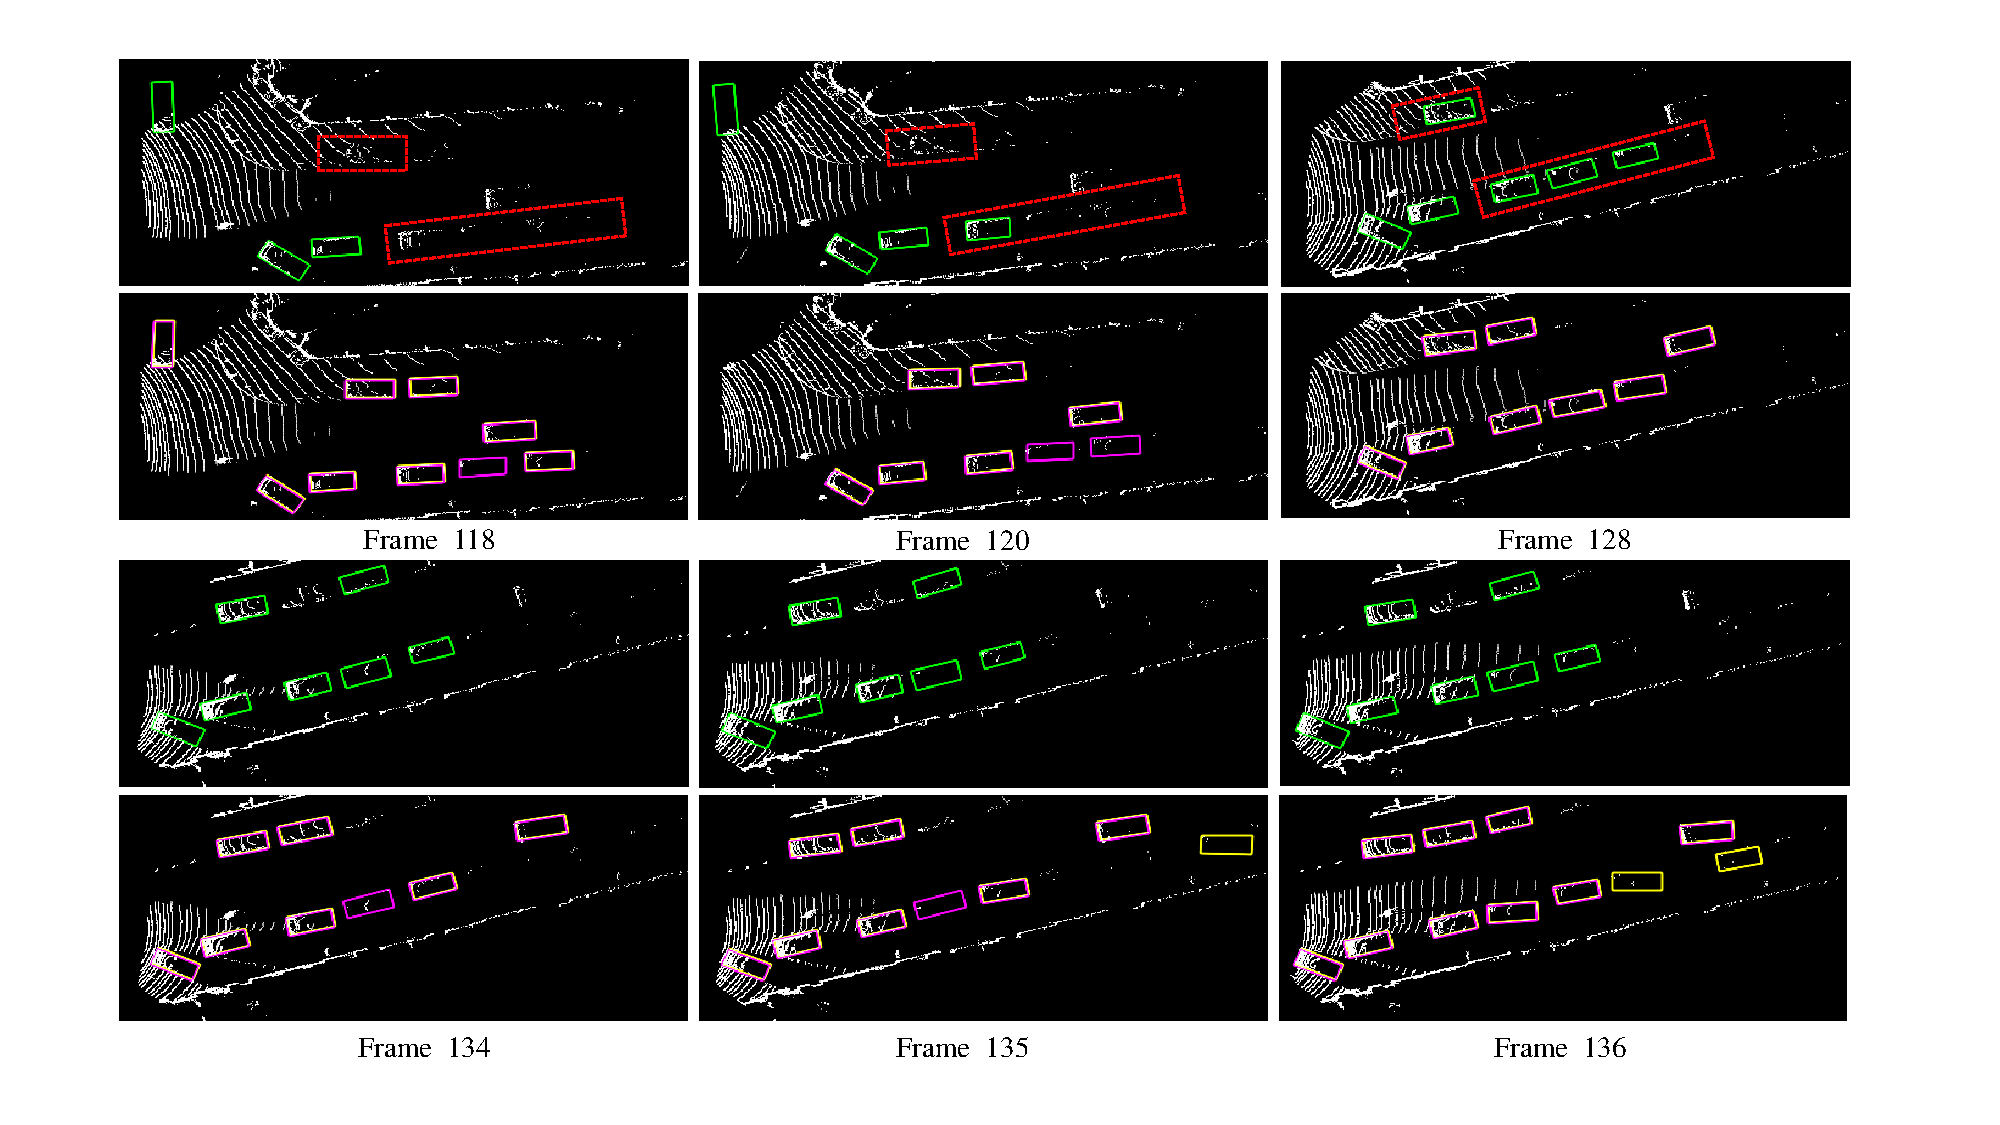
\includegraphics[trim={2cm, 1cm, 2.5cm, 1cm}, clip, width=\textwidth]{./imgs/examples.pdf}
	\vspace{-1.0cm}
	\caption{视频序列0的标签以及预测结果可视化。\textcolor{green}{绿色}为官方提供的标签框, \textcolor{yellow}{黄色}是时序步长$\tau = 1$的预测结果,\textcolor{magenta}{洋红色}为时序步长$\tau = 3$的预测结果。混合颜色的框是黄色框和洋红色框重叠造成的,该结果最好彩色打印查看。}
	\label{fig:examples}
\end{figure}


\subsection{多目标跟踪实验分析}
\label{mot_result}

\begin{table}
	\centering
	\wuhao
	\caption{DODT的不同设置在KITTI多目标追踪验证数据集上的结果。S 表示\textit{Shared RPN}模块, T 表示时序信息处理模块, M 表示运动插值模块。 $\tau$ 是关键帧选取时间步长。}
	\vspace{0.3cm}
	\resizebox{\textwidth}{!}{
		\begin{tabular}{cccccccc}
			\toprule[1.5pt]
			方法   & 模块 & MOTA(\%)$\uparrow$ & MOTP(\%)$\uparrow$ & MT(\%)$\uparrow$ & ML(\%)$\downarrow$ & IDS$\downarrow$&  FM$\downarrow$ \\ \midrule
			AVOD\cite{ku2018joint}    & -      & 66.05    & 82.97    & 46.22  & 12.18  & \textbf{2}      &  113  \\
			DODT($\tau$ = 3)          & S      & 76.53    & \textbf{83.93}    & 68.91  & 7.14   & 32      &  80  \\
			DODT($\tau$ = 3)          & S+T      & 77.52    & 83.75    & 69.33  & 7.56   & 37     &  77  \\
			DODT($\tau$ = 3)          & S+M      & 78.73    & \textbf{83.93}    & 68.49  & 9.55   & \textbf{2}      &  \textbf{48}  \\
			DODT($\tau$ = 3)  & S+T+M    & \textbf{79.72}   & 83.55    & \textbf{71.85}  & \textbf{5.46}  & 7  &  66  \\ 
			\bottomrule[1.5pt]
	\end{tabular}}
	\label{table:result_tracking}
\end{table}


\begin{table}
	\centering
	\wuhao
	\resizebox{\textwidth}{!}{
		\begin{tabular}{cccccccc}
			\toprule[1pt]
			方法    & MOTA(\%)$\uparrow$ & MOTP(\%)$\uparrow$ & MT(\%)$\uparrow$ & ML(\%)$\downarrow$ & IDS$\downarrow$&  FM$\downarrow$ &FPS$\uparrow$ \\ \midrule
			DSM\cite{frossard2018end}                         & 76.15    & 83.42    & 60.00  & 8.31  & 296  & 868  & 10.0 (GPU)  \\ %DSM
			3DT\cite{Hu3DT19} 	                              & \textbf{84.52}    & \textbf{85.64}	& \textbf{73.38}  & \textbf{2.77}  & 377  & 847  & 33.3 \\ %3DT
			Complexer-YOLO\cite{Simon_2019_CVPR_Workshops}    & 75.70    & 78.46    & 58.00  & 5.08  & 1186 & 2096 & \textbf{100.0} \\ %Complexer-YOLO
			3D-CNN/PMBM\cite{scheidegger2018mono}             & 80.39    & 81.26	& 62.77  & 6.15  & 121  & 613  & 71.4 \\  %3D-CNN/PMBM
			DODT(ours)                                        & 76.68    & 81.65    & 60.77  & 11.69 & \textbf{63}   & \textbf{384}  & 76.9 \\ 
			\bottomrule[1pt]
	\end{tabular}}
	\caption{DODT与现有的前沿方法在KITTI三维多目标追踪公开排行榜中的对比。FPS的计算不包含目标检测时间。}
	\label{label:result_kitti}
\end{table}



\section{结果展示}
\label{show}

\section{本章总结}
\label{exp_conclusion}


% 打印时插入必要的空白页
\ifprint
	\newpage
	\thispagestyle{empty}
	\mbox{}
	
	% 避免空白页影响页码编号
	\clearpage
	\setcounter{page}{10}
\fi
	% !Mode:: "TeX:UTF-8"

\chapter{结果展示}
\label{ch:results}

本章将选择DODT在KITTI追踪数据集上的一些结果进行展示,以便读者能够更好的了解DODT的性能。

\section{验证集结果展示}
\label{val_results}
本小节我们将可视化AVOD模型、Based\_DODT模型、DODT(T=1) 模型以及DODT(T=3) 模型在KITTI追踪验证数据集上的运行结果。我们将在同一个场景下绘制 AVOD与DODT(T=3) 、DODT(T=1)与DODT(T=3) 以及Based\_DODT 与 DODT(T=3)  这三对模型的对比结果,最好彩色打印查看。

\section{测试集结果展示}
\label{test_results}

本小节我们选择了KITTI追踪测试数据集中四段视频的连续四帧进行可视化,有BEV视角,3D视角以及图像视角。相同颜色表示同一辆车在不同时间的状态,最好彩色打印查看。

\begin{figure}
	\subfigure{
	\begin{minipage}[b]{0.4\linewidth}
		\begin{flushright}
			\begin{overpic}[scale=0.26]{./imgs/viz_results/06/bev/04.png}
				\put(5, 85){\color{red}{\small T = 3}}
			\end{overpic}\vspace{1pt}
			\begin{overpic}[scale=0.26]{./imgs/viz_results/06/bev/03.png}
				\put(5, 85){\color{red}{\small T = 2}}
			\end{overpic}\vspace{1pt}
			\begin{overpic}[scale=0.26]{./imgs/viz_results/06/bev/02.png}
				\put(5, 85){\color{red}{\small T = 1}}
			\end{overpic}\vspace{1pt}
			\begin{overpic}[scale=0.26]{./imgs/viz_results/06/bev/01.png}
				\put(5, 85){\color{red}{\small T = 0}}
			\end{overpic}
		\end{flushright}
	\end{minipage}}
	\subfigure{
	\begin{minipage}[b]{0.55\linewidth}
	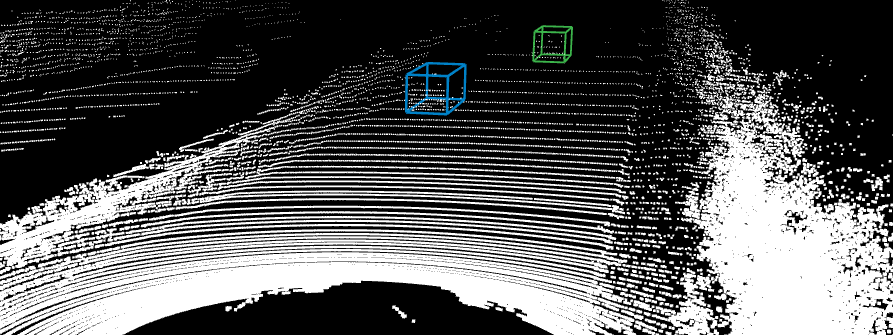
\includegraphics[width=1\linewidth]{./imgs/viz_results/06/pc/04.png}\vspace{1pt}
	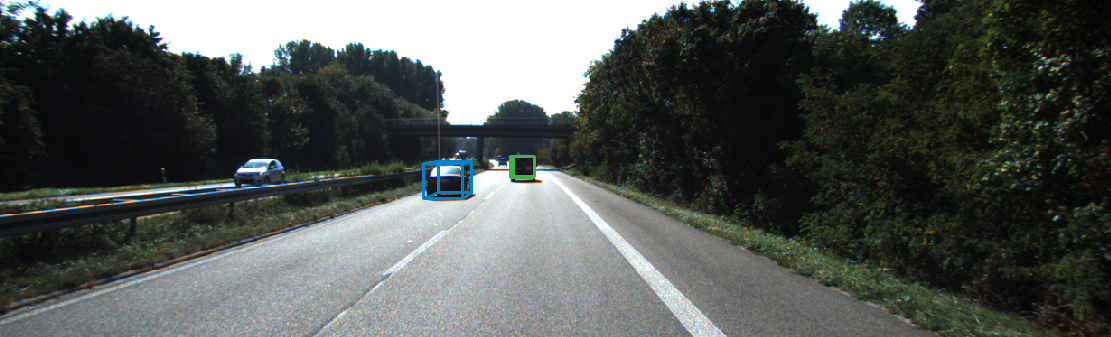
\includegraphics[width=1\linewidth]{./imgs/viz_results/06/img/04.png}\vspace{3.55pt}
	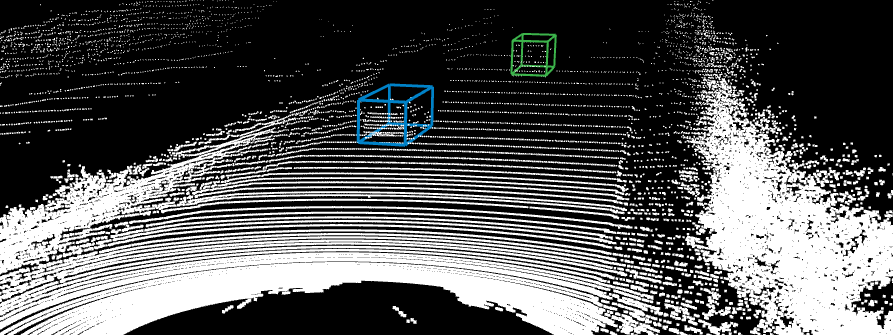
\includegraphics[width=1\linewidth]{./imgs/viz_results/06/pc/03.png}\vspace{1pt}
	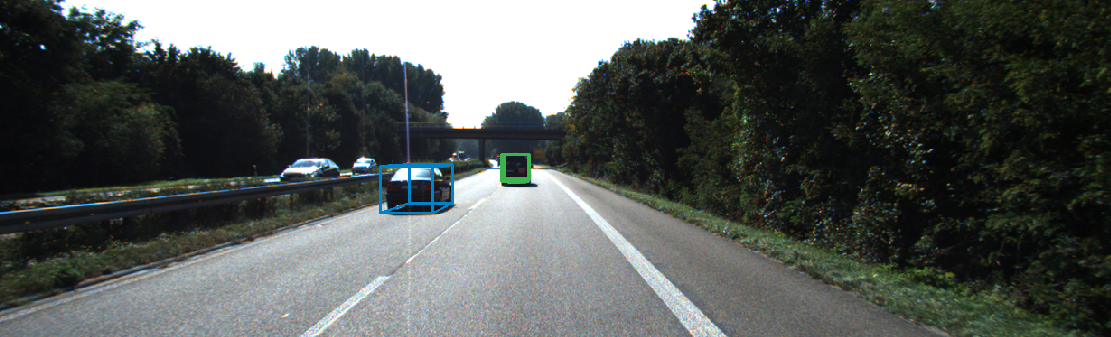
\includegraphics[width=1\linewidth]{./imgs/viz_results/06/img/03.png}\vspace{3.55pt}
	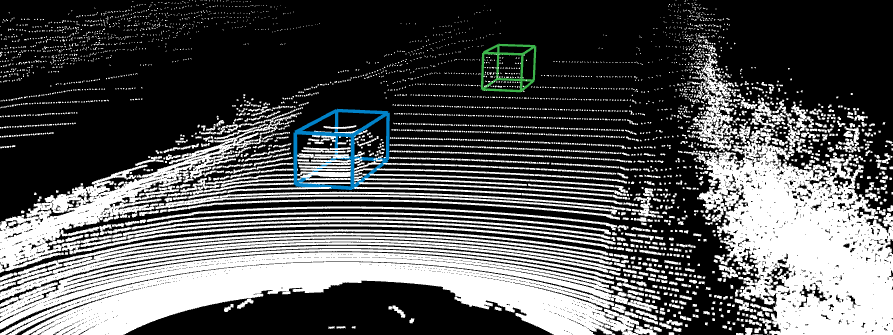
\includegraphics[width=1\linewidth]{./imgs/viz_results/06/pc/02.png}\vspace{1pt}
	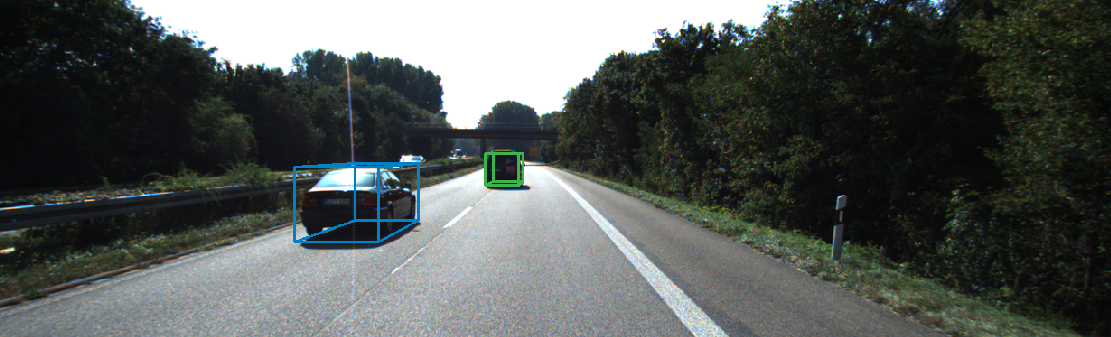
\includegraphics[width=1\linewidth]{./imgs/viz_results/06/img/02.png}\vspace{3.55pt}
	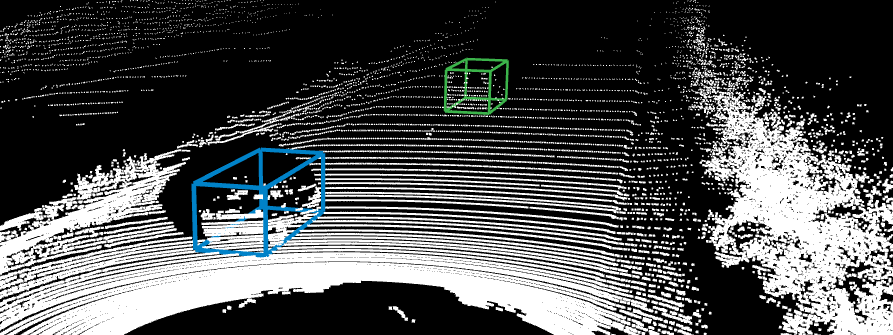
\includegraphics[width=1\linewidth]{./imgs/viz_results/06/pc/01.png}\vspace{1pt}
	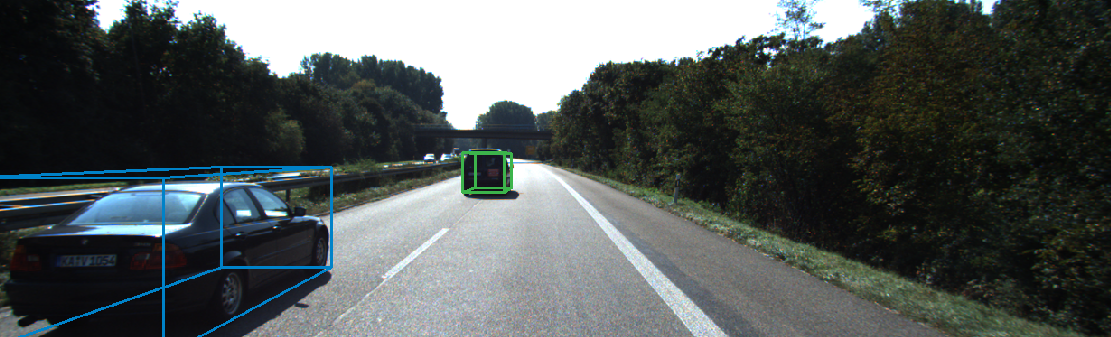
\includegraphics[width=1\linewidth]{./imgs/viz_results/06/img/01.png}
	\end{minipage}}
	\caption{KITTI多目标追踪测试集视频片段6的一段轨迹结果。}
\end{figure}

\begin{figure}
	\centering
	\subfigure{
		\begin{minipage}[b]{0.45\linewidth}
			\begin{overpic}[scale=0.230]{./imgs/viz_results/10/bev/04.png}
				\put(5, 55){\color{red}{\small T = 3}}
			\end{overpic}\vspace{4pt}
			\begin{overpic}[scale=0.230]{./imgs/viz_results/10/bev/03.png}
				\put(5, 55){\color{red}{\small T = 2}}
			\end{overpic}\vspace{4pt}
			\begin{overpic}[scale=0.230]{./imgs/viz_results/10/bev/02.png}
				\put(5, 55){\color{red}{\small T = 1}}
			\end{overpic}\vspace{4pt}
			\begin{overpic}[scale=0.230]{./imgs/viz_results/10/bev/01.png}
				\put(5, 55){\color{red}{\small T = 0}}
			\end{overpic}
	\end{minipage}}
	\subfigure{
		\begin{minipage}[b]{0.47\linewidth}
			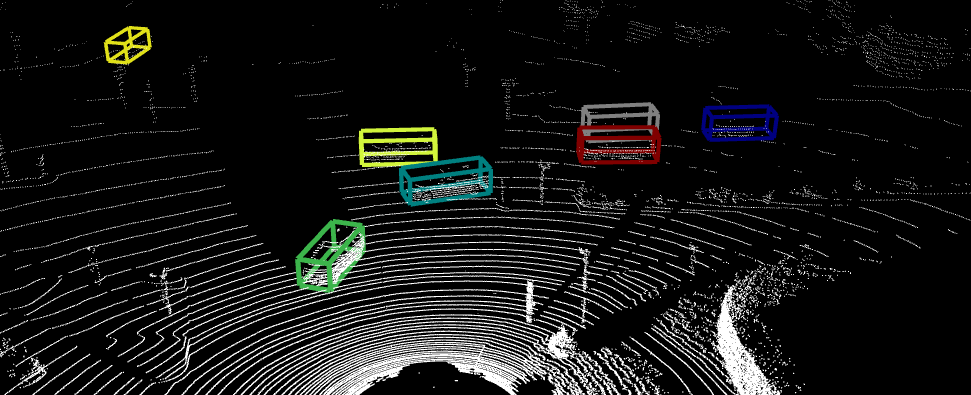
\includegraphics[width=1\linewidth]{./imgs/viz_results/10/pc/04.png}\vspace{1pt}
			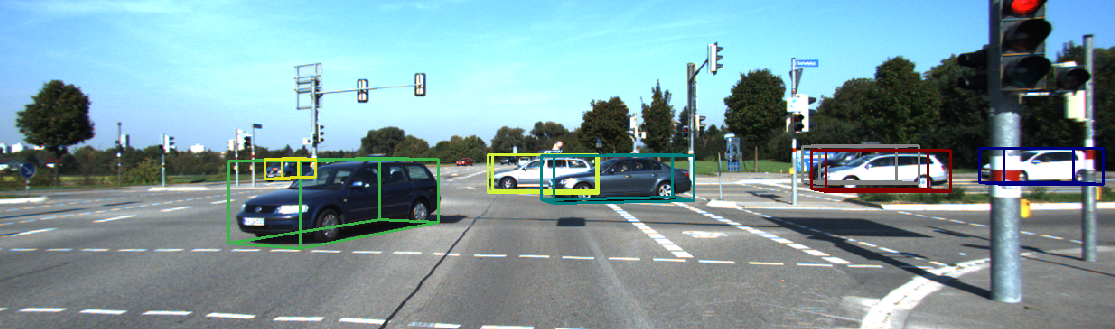
\includegraphics[width=1\linewidth]{./imgs/viz_results/10/img/04.png}\vspace{2.5pt}
			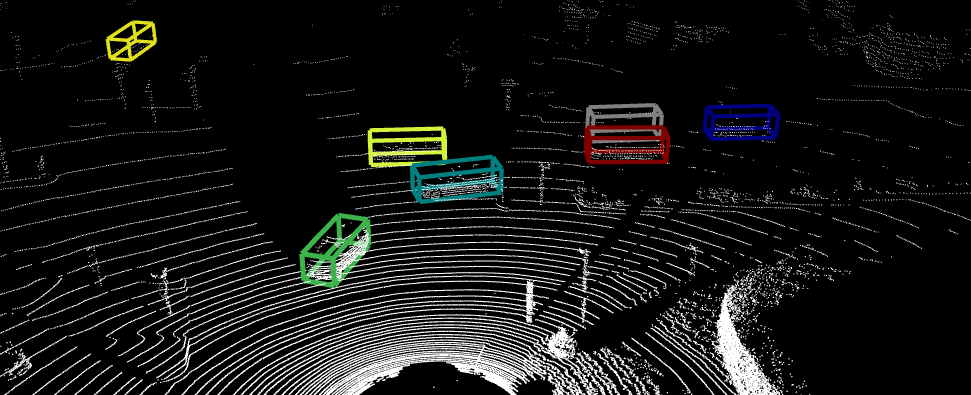
\includegraphics[width=1\linewidth]{./imgs/viz_results/10/pc/03.png}\vspace{1pt}
			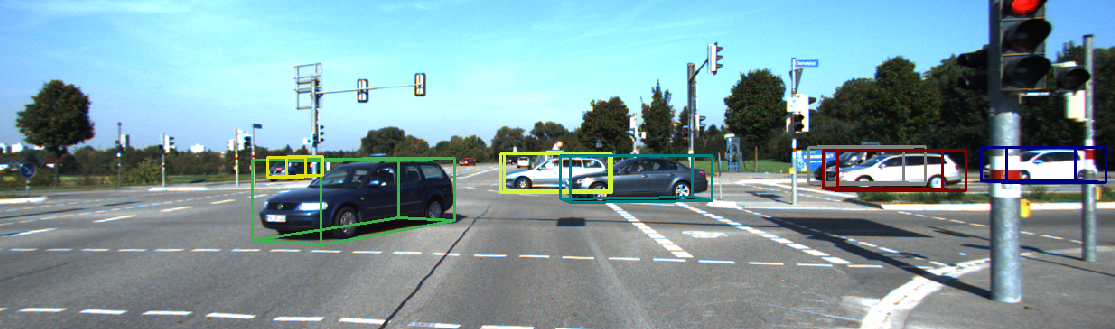
\includegraphics[width=1\linewidth]{./imgs/viz_results/10/img/03.png}\vspace{2.5pt}
			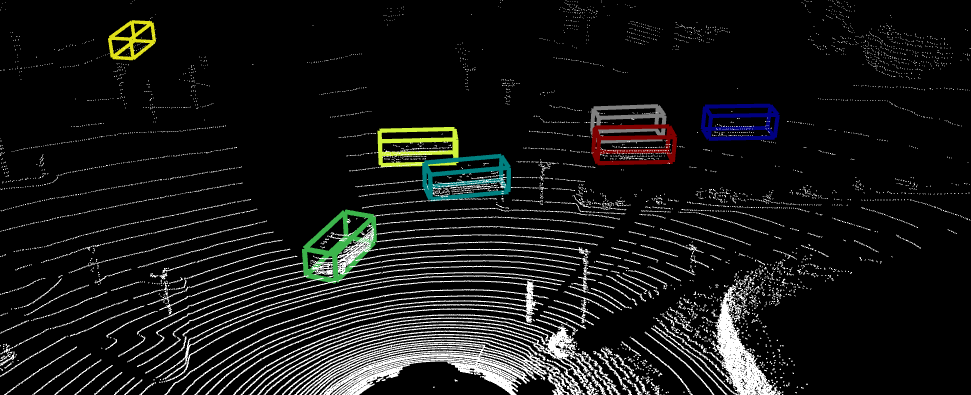
\includegraphics[width=1\linewidth]{./imgs/viz_results/10/pc/02.png}\vspace{1pt}
			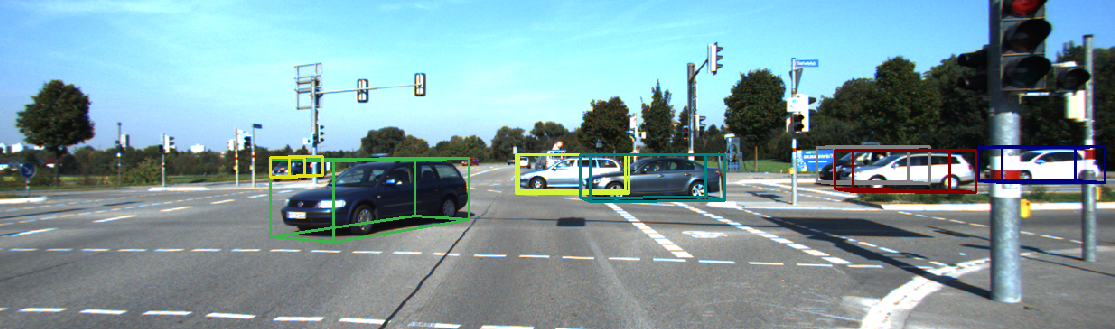
\includegraphics[width=1\linewidth]{./imgs/viz_results/10/img/02.png}\vspace{2.5pt}
			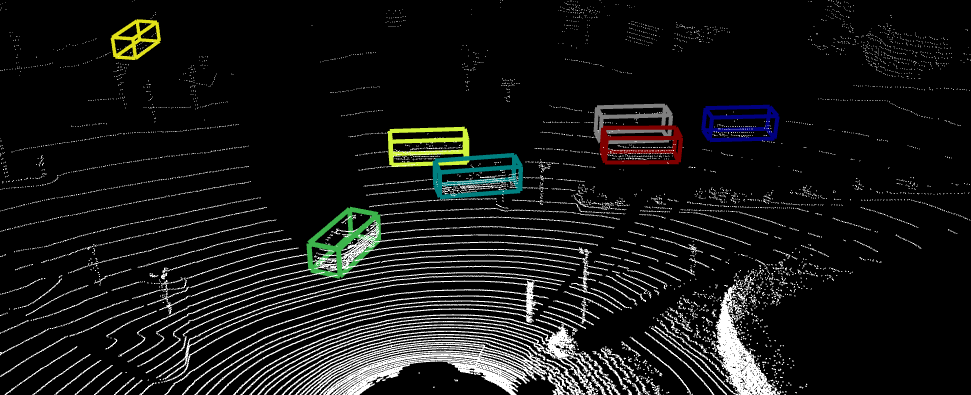
\includegraphics[width=1\linewidth]{./imgs/viz_results/10/pc/01.png}\vspace{1pt}
			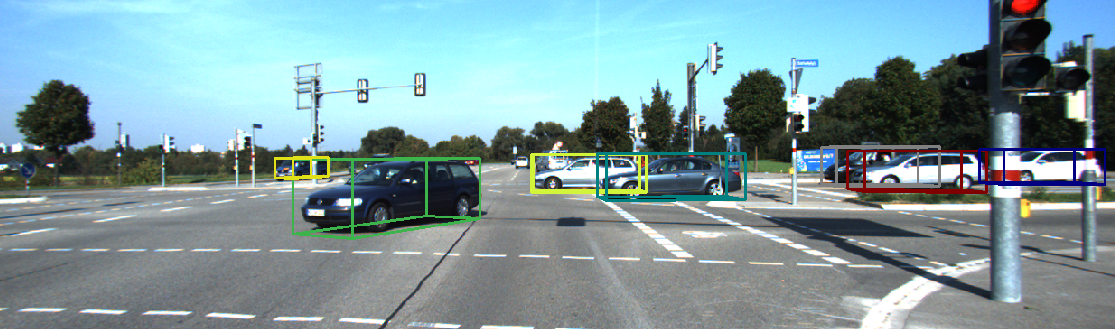
\includegraphics[width=1\linewidth]{./imgs/viz_results/10/img/01.png}
	\end{minipage}}
	\caption{KITTI多目标追踪测试集视频片段10的一段轨迹结果。}
\end{figure}

\begin{figure}
	%\centering
	\subfigure{
	\begin{minipage}[b]{0.4\linewidth}
	\begin{flushright}
		\begin{overpic}[trim={0cm, 3cm, 0cm, 0cm}, clip, scale=0.22]{./imgs/viz_results/11/bev/04.png}
			\put(5, 88){\color{red}{\small T = 3}}
		\end{overpic}\vspace{3pt}
		\begin{overpic}[trim={0cm, 3cm, 0cm, 0cm}, clip, scale=0.22]{./imgs/viz_results/11/bev/03.png}
			\put(5, 88){\color{red}{\small T = 2}}
		\end{overpic}\vspace{3pt}
		\begin{overpic}[trim={0cm, 3cm, 0cm, 0cm}, clip, scale=0.22]{./imgs/viz_results/11/bev/02.png}
			\put(5, 88){\color{red}{\small T = 1}}
		\end{overpic}\vspace{3pt}
		\begin{overpic}[trim={0cm, 3cm, 0cm, 0cm}, clip, scale=0.22]{./imgs/viz_results/11/bev/01.png}
			\put(5, 88){\color{red}{\small T = 0}}
		\end{overpic}
	\end{flushright}
	
	\end{minipage}}
	\subfigure{
	\begin{minipage}[b]{0.5\linewidth}
	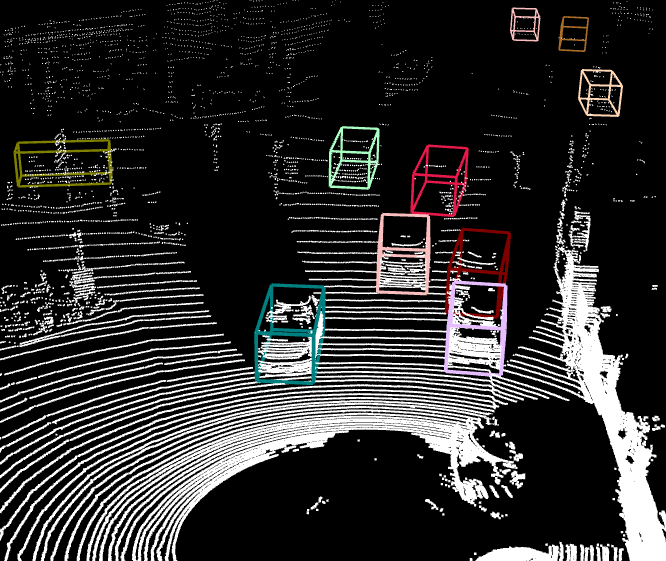
\includegraphics[trim={0cm, 5.5cm, 0cm, 0cm}, clip,width=0.85\linewidth]{./imgs/viz_results/11/pc/04.png}\vspace{1pt}
	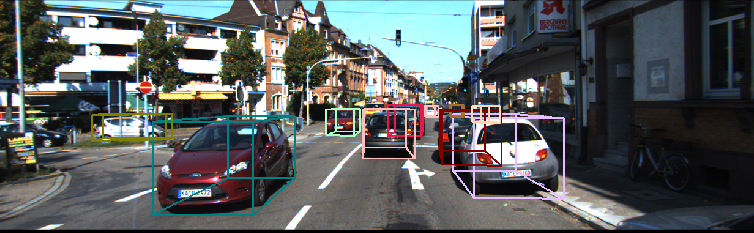
\includegraphics[width=0.85\linewidth]{./imgs/viz_results/11/img/04.png}\vspace{1.5pt}
	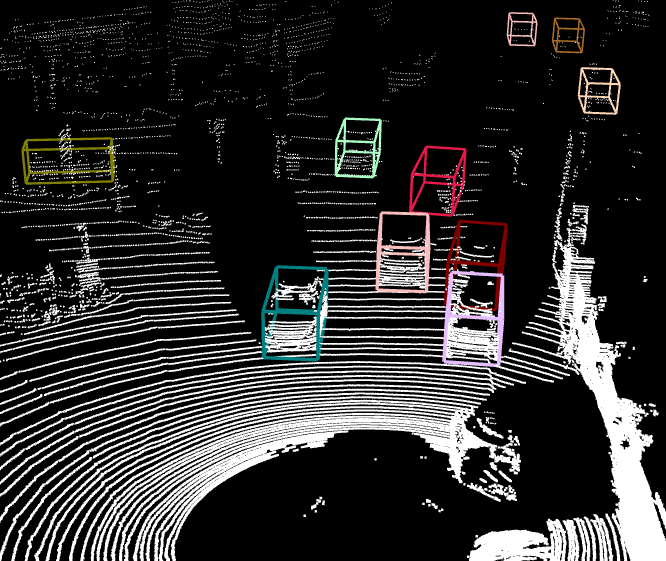
\includegraphics[trim={0cm, 5.5cm, 0cm, 0cm}, clip,width=0.85\linewidth]{./imgs/viz_results/11/pc/03.png}\vspace{1pt}
	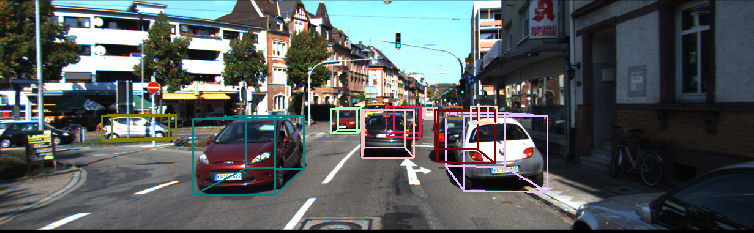
\includegraphics[width=0.85\linewidth]{./imgs/viz_results/11/img/03.png}\vspace{1.5pt}
	\includegraphics[trim={0cm, 5.5cm, 0cm, 0cm}, clip,width=0.85\linewidth]{./imgs/viz_results/11/pc/02.png}\vspace{1pt}
	\includegraphics[width=0.85\linewidth]{./imgs/viz_results/11/img/02.png}\vspace{1.5pt}
	\includegraphics[trim={0cm, 5.5cm, 0cm, 0cm}, clip,width=0.85\linewidth]{./imgs/viz_results/11/pc/01.png}\vspace{1pt}
	\includegraphics[width=0.85\linewidth]{./imgs/viz_results/11/img/01.png}
	\end{minipage}}
	\caption{KITTI多目标追踪测试集视频片段11的一段轨迹结果。}
\end{figure}


\begin{figure}
	\centering
	\subfigure{
	\begin{minipage}[b]{0.42\linewidth}
	\begin{flushright}
		\begin{overpic}[scale=0.221]{./imgs/viz_results/12/bev/04.png}
			\put(5, 87){\color{red}{\small T = 3}}
		\end{overpic}\vspace{3pt}
		\begin{overpic}[scale=0.221]{./imgs/viz_results/12/bev/03.png}
			\put(5, 87){\color{red}{\small T = 2}}
		\end{overpic}\vspace{3pt}
		\begin{overpic}[scale=0.221]{./imgs/viz_results/12/bev/02.png}
			\put(5, 87){\color{red}{\small T = 1}}
		\end{overpic}\vspace{3pt}
		\begin{overpic}[scale=0.221]{./imgs/viz_results/12/bev/01.png}
			\put(5, 87){\color{red}{\small T = 0}}
		\end{overpic}
	\end{flushright}
	\end{minipage}}
	\subfigure{
	\begin{minipage}[b]{0.55\linewidth}
	\includegraphics[width=\linewidth]{./imgs/viz_results/12/pc/04.png}\vspace{1pt}
	\includegraphics[width=\linewidth]{./imgs/viz_results/12/img/04.png}\vspace{1.5pt}
	\includegraphics[width=\linewidth]{./imgs/viz_results/12/pc/03.png}\vspace{1pt}
	\includegraphics[width=\linewidth]{./imgs/viz_results/12/img/03.png}\vspace{1.5pt}
	\includegraphics[width=\linewidth]{./imgs/viz_results/12/pc/02.png}\vspace{1pt}
	\includegraphics[width=\linewidth]{./imgs/viz_results/12/img/02.png}\vspace{1.5pt}
	\includegraphics[width=\linewidth]{./imgs/viz_results/12/pc/01.png}\vspace{1pt}
	\includegraphics[width=\linewidth]{./imgs/viz_results/12/img/01.png}
	\end{minipage}}
	\caption{KITTI多目标追踪测试集视频片段12的一段轨迹结果。}
\end{figure}


% 打印时插入必要的空白页
\ifprint
	\newpage
	\thispagestyle{empty}
	\mbox{}
	
	% 避免空白页影响页码编号
	\clearpage
	\setcounter{page}{10}
\fi

	% !Mode:: "TeX:UTF-8"
\chapter{总结与展望}
\label{conclusion}

\section{全文总结}
\label{summary}
本工作提出了一个双路物体检测与跟踪(Dual-way Object Detection and Tracking, DODT)框架, 旨在将三维物体检测从单帧推广到多帧连续场景,从而推动前沿三维物体检测算法在自动驾驶领域的落地。DODT的主要思想是基于流数据的连续性以及冗余性,通过只对关键帧做物体检测,然后在时序信息的引导下将关键帧检测结果传播到非关键帧,最后再将帧间数据关联,完成三维物体检测与多目标追踪任务。在该思想的引导下,本文分了五部分详细介绍了DODT的研究背景、研究基础、原理实现、实验验证以及结果展示。在第一章中,本文详细阐述了近年来国内外在三维目标检测领域的进展,并分析了各流派的优缺点,以及将单帧方法推广到多帧流数据场景的重要意义。第二章则详细介绍了基于深度学习技术的目标检测技术进展,重点介绍了以Faster-RCNN为代表的两阶段目标检测以及以YOLO为代表的单阶段目标检测的原理和实现方式,为读者了解DODT的原理提供技术参考。之后本章还简要介绍了单目标追踪的方法原理,以及多目标追踪的研究进展以及性能衡量指标。本文第三章开始重点介绍了DODT的网络架构与实现原理,先后详细介绍了组成DODT的四个基本模块:三维物体检测模块、\textit{Shared RPN}模块、时序信息处理模块和运动插值模块,以及这些模块如何相互配合完成流数据的物体检测与多目标跟踪任务。第四章阐述了DODT的实验验证环节,该章首先介绍了实验所用的KITTI数据集以及数据预处理步骤,然后使用控制变量法分析了DODT个模块对最终检测与追踪性能的影响,并分析出了最佳的关键帧选取步长。另外,该章还介绍了DODT在三维多目标追踪领域与前沿方法的性能对比,实验结果表明DODT能够取得与前沿方法匹敌的性能,并且有着自己的独特优势。本文第五章展示了一些可视化结果,有在验证集下各模型的可视化对比,也有DODT在测试集下的预测结果,希望能够为读者提供关于DODT模型性能更形象化的了解。


\section{展望}
\label{future}
DODT虽然在流数据物体检测与跟踪任务取得了显著的效果,但它离运用到自动驾驶平台还有很长一段距离。DODT框架的落地还需要解决以下四个问题:
\begin{itemize}
\item 目前的检测模型只局限于AVOD网路,能否将其扩展到任何三维物体检测模型,例如目前PointRCNN系列检测框架?
\item 目前DODT是以近似在线跟踪的方式实现多目标跟踪,能否在DODT的基础上设计出在线的三维多目标跟踪算法?
\item DODT模型在长关键帧选取步长上效果不佳,是否有更为有效的关键帧选取算法?以及是否有更加高效的时序信息提取方法?
\item DODT框架要落地还需进一步提升速度,能否使用模型压缩方法进一步提高模型的运行效率,使其能够迁移到嵌入式设备上?
\end{itemize}
本项目后续工作将重点从这四个方面入手,继续改进现有的DODT框架。对于第一个问题,设计适应性更广、扩展性更强的DODT框架,目前我们已开展相关工作。由于三维物体检测领域算法日新月异,目前KITTI排行榜的前几位算法都是只基于点云数据的,并且也有先进行点云分割再回归目标框的算法。因此扩展版的DODT应将这些算法囊括进来,构建一个通用的三维流数据物体检测框架。在该基础上,在线多目标跟踪算法、关键帧选取算法以及更加高效的时序信息提取算法的探索可以同步进行。DODT的嵌入式迁移是本项目最后的工作,目前我们考虑了参数压缩以及二值化网络的方案。只有将DODT在嵌入式设备上运行,才能够真正意义上实现算法落地,推进自动驾驶领域的技术革新。

% 打印时插入必要的空白页
\ifprint
	\newpage
	\thispagestyle{empty}
	\mbox{}
	
	% 避免空白页影响页码编号
	\clearpage
	\setcounter{page}{10}
\fi
	
	% 覆盖设置参考文献等后续页面样式
	\clearpage
	\defaultfont
	\lhead{}
	\rhead{}
	\chead{\song\wuhao 中山大学硕士学位论文}
	% ——————————————————————————————————————————————
	% 以下是论文参考文献,在references子文件下
	
	% 设置参考文献四字的格式
	\titleformat{\chapter}{\centering\sanhao\hei}{}{2em}{}
	
	%%%%%%%%%%  参考文献  %%%%%%%%%%
	\bibliographystyle{styles/TJUThesis}
	\phantomsection
	\markboth{参考文献}{参考文献}
	% 参考文献加入到中文目录
	\addcontentsline{toc}{chapter}{参考文献}
	% 若将此命令屏蔽掉,则未引用的文献不会出现在文后的参考文献中
	%\nocite{*}
	\bibliography{references/thesis}
	
	% ——————————————————————————————————————————————
	% 以下是论文附录,在appendix子文件下
	% 重新设置想要的chapter格式: 去掉章节序号
	\titleformat{\chapter}{\centering\sihao\hei}{}{2em}{}
	
	% 攻读硕士学位期间发表学术论文情况
	% !Mode:: "TeX:UTF-8"

% 打印时插入必要的空白页
\ifprint
	\newpage
	\thispagestyle{empty}
	\mbox{}
	
	% 避免空白页影响页码编号
	\clearpage
	\setcounter{page}{10}
\fi

\markboth{攻读硕士学位期间发表学术论文情况}{攻读硕士学位期间发表学术论文情况}
\addcontentsline{toc}{chapter}{攻读硕士学位期间发表学术论文情况}
% 如果需要从该页开始从 1 开始编页,则取消以下注释
%\setcounter{page}{1}
\chapter*{攻读硕士学位期间发表学术论文情况}

\begin{enumerate}
	% 盲审时
	\item The paper title [J/C...]. Publish whereabout, 2014, 21(3): 288-291. (第一作者,导师为第一作者)(与学位论文第n章相关)(盲审时,不要出现名字)
	% 提交时
	\item Authors. The paper title [J/C...]. Publish whereabout, 2014, 21(3): 288-291. (提交时)
\end{enumerate}

% 不显示页码,则取消以下注释
%\thispagestyle{empty}


% 打印时插入必要的空白页
\ifprint
	\newpage
	\thispagestyle{empty}
	\mbox{}
	
	% 避免空白页影响页码编号
	\clearpage
	\setcounter{page}{10}
\fi
	
	% 致谢
	% !Mode:: "TeX:UTF-8"

\markboth{致\quad 谢}{致\quad 谢}
\addcontentsline{toc}{chapter}{致\quad 谢} % 添加到目录中
\chapter*{致\quad 谢}

谨此向我的导师张三教授致以衷心的感谢和崇高的敬意!本论文的工作是在张老师的悉心指导下完成的。在传授予我专业知识和宝贵经验的同时,张老师以其严谨的治学态度和精益求精的工作作风不断促进论文相关工作的进行,使我受益匪浅。
 
在攻读硕士的这三年里,导师和实验室的同学们不仅为我创造了优越的科研和学习环境,使我得以在计算机科学领域中自由翱翔,同时在思想上、人生态度和意志品质方面给予了谆谆教诲,这些教益必将激励着我在今后的人生道路上奋勇向前。特别感谢实验室的甲师兄、乙同学以及其他师弟师妹,他们不仅在学术上给了我许多指引和建议,而且在生活上予以帮助,从他们身上我学到了很多知识。

感谢王五老师及其实验室的同学在领域一、领域二方面的学习给予我的帮助。他们开创性的研究拓展了我的学术视野,无数次的争论和探讨使我的研究工作有了长足的进展。

由衷感谢我的室友A、B和C同学,以及其他经常到我们宿舍进行学习交流的D、E、F和G同学,是他们令我的学习生活都更加充满动力。
衷心的感谢我的父母和其他亲朋好友对我的关心、支持和理解,没有他们对我的关心、鼓励和支持,我无法完成现在的硕士学业。 

最后,感谢所有曾经教育和帮助过我的所有老师。衷心地感谢为评阅本论文而付出宝贵时间和辛勤劳动的专家和教授们!

% 如果需要加名字和日期(日期根据生成文档日期变更)
\maketime


	
	\clearpage
	% 结束全文
\end{document}